\documentclass[a4paper,11pt]{book}
%\documentclass[a4paper,twoside,11pt,titlepage]{book}
\usepackage{listings}
\usepackage{courier}
\lstset{
    basicstyle=\footnotesize\ttfamily, % Default font
    numbers=left,              % Location of line numbers
    numberstyle=\tiny,          % Style of line numbers
    stepnumber=2,              % Margin between line numbers
    numbersep=5pt,              % Margin between line numbers and text
    tabsize=2,                  % Size of tabs
    extendedchars=true,
    breaklines=true,            % Lines will be wrapped
    keywordstyle=\color{red},
    frame=b,
    keywordstyle=[1]\textbf,
    keywordstyle=[2]\textbf,
    % keywordstyle=[3]\textbf,
    % keywordstyle=[4]\textbf,   \sqrt{\sqrt{}}
    stringstyle=\color{white}\ttfamily, % Color of strings
    showspaces=false,
    showtabs=false,
    xleftmargin=17pt,
    framexleftmargin=17pt,
    framexrightmargin=5pt,
    framexbottommargin=4pt,
    % backgroundcolor=\color{lightgray},
    showstringspaces=false
}
\lstloadlanguages{ % Check documentation for further languages ...
     % [Visual]Basic,
     % Pascal,
     % C,
     % C++,
     % XML,
     % HTML,
     Java
}
\usepackage[utf8]{inputenc}
\usepackage[spanish]{babel}
\addto\captionsspanish{%
%\def\bibname{Referencias}%
\def\tablename{Tabla}%
}
\usepackage[gen]{eurosym}

\usepackage[
backend=biber,
style=alphabetic,
sorting=ynt
]{biblatex}

\addbibresource{bibliografia.bib}

\usepackage{caption}
\DeclareCaptionFont{white}{\color{white}}
\DeclareCaptionFormat{listing}{\colorbox[cmyk]{0.43, 0.35, 0.35,0.01}{\parbox{\textwidth}{\hspace{15pt}#1#2#3}}}
\captionsetup[lstlisting]{format=listing,labelfont=white,textfont=white, singlelinecheck=false, margin=0pt, font={bf,footnotesize}}



\usepackage{tcolorbox}

% \usepackage[style=list, number=none]{glossary} %
%\usepackage{titlesec}
%\usepackage{pailatino}

\decimalpoint
\usepackage{dcolumn}
\newcolumntype{.}{D{.}{\esperiod}{-1}}
\makeatletter
\addto\shorthandsspanish{\let\esperiod\es@period@code}
\makeatother


%\usepackage[chapter]{algorithm}
\RequirePackage{verbatim}
%\RequirePackage[Glenn]{fncychap}
\usepackage{fancyhdr}
\usepackage{graphicx}
\usepackage{afterpage}
\usepackage[section]{placeins}
\usepackage{longtable}

\usepackage[hidelinks]{hyperref}
\usepackage{glossaries}

\makeglossaries

\newglossaryentry{Malware}
{
    name=Malware,
    description={O software  `malicioso' es todo aquél programa o código que pretende (de forma intencionada) causar daños y/o sacar beneficios de un sistema}
}

\newglossaryentry{cloud}
{
    name=Cloud,
    description={La computación en la nube o \textit{cloud} (del inglés cloud computing), conocida también como servicios en la nube, informática en la nube, nube de cómputo o simplemente «la nube», es un paradigma que permite ofrecer servicios de computación a través de una red, que usualmente es internet}
}

\newglossaryentry{Ransomware}
{
    name=Ransomware,
    description={Es un tipo de \gls{Malware} que hace públicos o inaccesibles (por medio de encriptación, por ejemplo) los datos de la víctima con el objetivo de chantajearla para que pague un `rescate'}
}


\newglossaryentry{Reverse engineering}
{
    name={ingeniería inversa},
    description={Es una técnica que consiste en tratar de obtener por medios deductivos información sobre un producto o sistema haciendo uso del mismo y tratando de figurar como está diseñado}
}

\newglossaryentry{obfuscation}{
    name={obfuscation},
    description={Ofuscación, ocultación, anonimato. Es el acto de evitar ser descubierto mientras se realiza un ataque o una auditoría. Bien eliminando los rastros que se puedan dejar u ocultándolos por medio de falsos rastros que los escodan}
}

\newglossaryentry{network sniffing}
{
    name=network sniffing,
    description={Es la acción de atrapar y atender a todo el tráfico indiscriminado que circula por una red, sea cual sea su destinatario, con el objetivo de obtener algún tipo de información de interés}
}

\newglossaryentry{Rolling Release}
{
    name=Rolling Release,
    description={Es un tipo de distribución de Software en el que las actualizaciones son continuas en lugar de depender de un versionado discreto. Los cambios se van añadiendo de forma incremental conforme van siendo disponibles en lugar de ir emitiendo nuevas versiones con todos los cambios desde la anterior}
}

\newglossaryentry{compliance} 
{
    name=compliance,
    description={'el cumplimiento' de las normativas o leyes referentes a la seguridad de los datos que una empresa pueda almacenar o gestionar}
}

\newglossaryentry{vagrant}
{
    name=Vagrant,
    description={'una herramienta diseñada para el despliegue y configuración de entornos de máquinas virtuales (utilizando diversos proveedores como virtualbox, qemu, aws, etc}
}

\newacronym{ddos}{DDOS}{Distributed Denial Of Service}

\newacronym{aws}{AWS}{Amazon Web Service}


\newacronym{iot}{IOT}{The Internet of Things}

\newglossaryentry{OpenSource}
{
    name=OpenSource,
    description={OpenSource o código abierto es un tipo de software liberado con una licencia que asegura el derecho de los usuarios a usar, estudiar, cambiar y distribuir el mismo con cualquier propósito}
}

\newglossaryentry{Pull Request}
{
    name=Pull Request,
    description={Una Pull Request es la acción de validar un código que se va a mergear de una rama a otra. Por ejemplo, de una rama de desarrollo en un Fork de un proyecto a una rama oficial}
}

\newglossaryentry{Fuzzing}
{
    name=Fuzzing,
    description={Según la OWASP, fuzzing es el acto de introducir datos mal formados en un programa con el objetivo de conseguir un comportamiento en este inesperado. Aplicado, por ejemplo, al ámbito de web, podríamos considerar fuzzing las técnicas de SQL injection y similares, dónde se introduce código SQL en lugares como los credenciales de acceso para conseguir logearse con un usuario distinto al que poseemos}
}

\newglossaryentry{syslog}
{
    name=Syslog,
    description={syslog es un estándar para el envío de mensajes de registro (logs) en una red informática IP. Por syslog se conoce tanto al protocolo de red como a la aplicación o biblioteca que envía los mensajes de registro. Un mensaje de registro suele tener información sobre la seguridad del sistema, aunque puede contener cualquier información. Junto con cada mensaje se incluye la fecha y hora del envío}
}

\newglossaryentry{phishing}
{
    name=Phishing,
    description={Técnica empleada por delincuente cibernéticos para estafar y obtener información de sus víctimas haciéndose pasar por otra persona o entidad (a través de correo electrónico, redes sociales, etc}
}


\newacronym{IaC}{IAC}{Infrastructure as Code}
\newacronym{CPA}{CPA}{Certified Public Accountant}
\newacronym{FOSS}{FOSS}{Free & Open-Source Software}

\newglossaryentry{forensics}
{
    name=forensics,
    description={Es el término que describe a las acciones llevadas a cabo para recopilar información de los sistemas informáticos que pueda ser utilizada para demostrar hechos por ejemplo durante una investigación relacionada con un crimen cibernético}
}

\newglossaryentry{antiforensics}
{
    name=anti-forensics,
    description={Técnicismo que se emplea para referise a aquellas acciones llevadas a cabo para dificultar las labores de investigación forense (forensics \gls{forensics}) de los equipos de seguridad de una empresa. Borrar u ocultar los rastros que se pueda haber dejado durante la explotación de vulnerabilidades de un sistema con el objetivo de imposibilitar el descubrimiento del mismo por parte de los administradores del sistema}
}

\newglossaryentry{siem}
{
    name=SIEM,
    description={`Security Information and Event Management', es un tipo de software que permite recopilar y analizar información de seguridad de distintos dispositivos, alertando al usuario de aquellos eventos importantes que tengan lugar}
}


\newglossaryentry{HIDS}
{
    name=HIDS,
    description={`Host Based Intrussion Detection System', es un tipo de software que permite detertar intentos de intrusiones en un sistema y reportarlas}
}

\newglossaryentry{mitre}
{
    name=MITRE ATT\&ACK,
    description={Una base de datos pública de conocimiento de tácticas de `ataques adversarios' que trata de modelar y agrupar las distintas acciones que puede llevar a cabo un criminar para dañar a una entidad}
}

\newglossaryentry{fork}
{
    name=fork,
    description={También llamado `bifurcación' en español. Es el desarrollo de un proyecto informático tomando como base el código fuente de uno ya existente o de alguna ramificación de este. Un ejemplo claro de esto son las distintas diburcaciones de desarrollo de las distribuciones de Linux, dónde Ubuntu, por ejemplo, es una bifurcación o un fork de Debian}
}

\newglossaryentry{reverse_shell}
{
    name=Consola inversa,
    description={O en inglés `reverse shell'. Es un tipo de conexión entre dos hosts que ocurre de forma opuesta a la habitual: desde el dispositivo que se va a conectar se abre una aplicación que `espera' una conexión y desde el dispositivo que va a ser accedido se abre una consola de comandos que se conecta a dicha aplicación. Es una técnica que se utiliza en el ámbito de la ciberseguridad para conseguir acceso remoto a dispositivos dónde podemos ejecutar código arbitrario de algún modo}
}

\newglossaryentry{bugb}
{
    name=Bug Bounty,
    description={Son programas en los que empresas u organizaciones ofrecen importantes recompensas económicas a aquellas personas (ajenas a la organización) capaces de encontrar vulnerabilidades o errores de seguridad en alguno de sus sistemas.}
}

% ********************************************************************
% Re-usable information
% ********************************************************************
\newcommand{\myTitle}{Integración de procesos de Hacking ético en la plataforma de ciberseguridad Wazuh \xspace}
\newcommand{\myDegree}{Grado en ingeniería informáticaxspace}
\newcommand{\myName}{Francisco Navarro Morales\xspace}
\newcommand{\myProf}{Alberto Guillén Perales\xspace}
%\newcommand{\mySupervisor}{Put name here\xspace}
\newcommand{\myFaculty}{Escuela Técnica Superior de Ingenierías Informática y de
Telecomunicación\xspace}
\newcommand{\myFacultyShort}{E.T.S. de Ingenierías Informática y de
Telecomunicación\xspace}
\newcommand{\myDepartment}{Departamento de ...\xspace}
\newcommand{\myUni}{\protect{Universidad de Granada}\xspace}
\newcommand{\myLocation}{Granada\xspace}
\newcommand{\myTime}{\today\xspace}
\newcommand{\myVersion}{Version 0.1\xspace}


%\hyphenation{}


%\usepackage{doxygen/doxygen}
%\usepackage{pdfpages}
\usepackage{url}
\usepackage{colortbl,longtable}
\usepackage[stable]{footmisc}
%\usepackage{index}

%\makeindex
%\usepackage[style=long, cols=2,border=plain,toc=true,number=none]{glossary}
% \makeglossary

% Definición de comandos que me son tiles:
%\renewcommand{\indexname}{Índice alfabético}
%\renewcommand{\glossaryname}{Glosario}

\pagestyle{fancy}
\fancyhf{}
\fancyhead[LO]{\leftmark}
\fancyhead[RE]{\rightmark}
\fancyhead[RO,LE]{\textbf{\thepage}}
\renewcommand{\chaptermark}[1]{\markboth{\textbf{#1}}{}}
\renewcommand{\sectionmark}[1]{\markright{\textbf{\thesection. #1}}}

\setlength{\headheight}{1.5\headheight}

\newcommand{\HRule}{\rule{\linewidth}{0.5mm}}
%Definimos los tipos teorema, ejemplo y definición podremos usar estos tipos
%simplemente poniendo \begin{teorema} \end{teorema} ...
\newtheorem{teorema}{Teorema}[chapter]
\newtheorem{ejemplo}{Ejemplo}[chapter]
\newtheorem{definicion}{Definición}[chapter]

\definecolor{gray97}{gray}{.97}
\definecolor{gray75}{gray}{.75}
\definecolor{gray45}{gray}{.45}
\definecolor{gray30}{gray}{.94}

\lstset{ frame=Ltb,
     framerule=0.5pt,
     aboveskip=0.5cm,
     framextopmargin=3pt,
     framexbottommargin=3pt,
     framexleftmargin=0.1cm,
     framesep=0pt,
     rulesep=.4pt,
     backgroundcolor=\color{gray97},
     rulesepcolor=\color{black},
     %
     stringstyle=\ttfamily,
     showstringspaces = false,
     basicstyle=\scriptsize\ttfamily,
     commentstyle=\color{gray45},
     keywordstyle=\bfseries,
     %
     numbers=left,
     numbersep=6pt,
     numberstyle=\tiny,
     numberfirstline = false,
     breaklines=true,
   }
 
% minimizar fragmentado de listados
\lstnewenvironment{listing}[1][]
   {\lstset{#1}\pagebreak[0]}{\pagebreak[0]}

\lstdefinestyle{CodigoC}
   {
	basicstyle=\scriptsize,
	frame=single,
	language=C,
	numbers=left
   }
\lstdefinestyle{CodigoC++}
   {
	basicstyle=\small,
	frame=single,
	backgroundcolor=\color{gray30},
	language=C++,
	numbers=left
   }

 
\lstdefinestyle{Consola}
   {basicstyle=\scriptsize\bf\ttfamily,
    backgroundcolor=\color{gray30},
    frame=single,
    numbers=none
   }


\newcommand{\bigrule}{\titlerule[0.5mm]}


%Para conseguir que en las páginas en blanco no ponga cabeceras
\makeatletter
\def\clearpage{%
  \ifvmode
    \ifnum \@dbltopnum =\m@ne
      \ifdim \pagetotal <\topskip
        \hbox{}
      \fi
    \fi
  \fi
  \newpage
  \thispagestyle{empty}
  \write\m@ne{}
  \vbox{}
  \penalty -\@Mi
}
\makeatother

\usepackage{pdfpages}
\begin{document}
\begin{titlepage}
 
 
\newlength{\centeroffset}
\setlength{\centeroffset}{-0.5\oddsidemargin}
\addtolength{\centeroffset}{0.5\evensidemargin}
\thispagestyle{empty}

\noindent\hspace*{\centeroffset}\begin{minipage}{\textwidth}

\centering

\includegraphics[width=0.7\textwidth]{imagenes/logo_ugr.jpg}\\[1.4cm]

\textsc{ \Large TRABAJO FIN DE GRADO\\[0.1cm]}
\textsc{ INGENIERÍA INFORMÁTICA}\\[0.6cm]
% Upper part of the page
% 
% Title
{\Huge\bfseries Integración de procesos de Hacking ético en la plataforma de ciberseguridad Wazuh \\
}
\noindent\rule[-1ex]{\textwidth}{3pt}\\[3.5ex]
{\large\bfseries Un estudio del rol de Wazuh en el ámbito de las auditorías de ciberseguridad y los tests de penetración de sistemas. Análisis y resolución del problema de monitorización de acciones en la consola de comandos y caso practico de la aplicación de las herramientas desarrolladas al hacking ético.}
\end{minipage}

\vspace{1.5cm}
\noindent\hspace*{\centeroffset}\begin{minipage}{\textwidth}
\centering

\textbf{Autor}\\ {Francisco Navarro Morales}\\[2.5ex]
\textbf{Director}\\
{Alberto Guillén Perales\\}

\includegraphics[width=0.3\textwidth]{imagenes/etsiit_logo.png}\\[0.1cm]
\textsc{Escuela Técnica Superior de Ingenierías Informática y de Telecomunicación}\\
\textsc{---}\\
Granada, Septiembre de 2020
\end{minipage}
%\addtolength{\textwidth}{\centeroffset}
%\vspace{\stretch{2}}
\end{titlepage}



\chapter*{}
%\thispagestyle{empty}
%\cleardoublepage

%\thispagestyle{empty}

\begin{titlepage}
 
 
\setlength{\centeroffset}{-0.5\oddsidemargin}
\addtolength{\centeroffset}{0.5\evensidemargin}
\thispagestyle{empty}

\noindent\hspace*{\centeroffset}\begin{minipage}{\textwidth}

\centering
%
\includegraphics[width=0.9\textwidth]{imagenes/logo_ugr.jpg}\\[1.4cm]

%\textsc{ \Large PROYECTO FIN DE CARRERA\\[0.2cm]}
%\textsc{ INGENIERÍA EN INFORMÁTICA}\\[1cm]
% Upper part of the page
% 

%si el proyecto tiene logo poner aquí

\includegraphics{imagenes/logo.png} 

% Title

{\Huge\bfseries Integración de procesos de Hacking ético en la plataforma de ciberseguridad Wazuh\\
}
\noindent\rule[-1ex]{\textwidth}{3pt}\\[3.5ex]
{\large\bfseries Un estudio del rol de Wazuh en el ámbito de las auditorías de ciberseguridad y los tests de penetración de sistemas. Análisis y resolución del problema de monitorización de acciones en la consola de comandos y caso practico de la aplicación de las herramientas desarrolladas al hacking ético.\\[4cm]}
\end{minipage}

\vspace{1.5cm}
\noindent\hspace*{\centeroffset}\begin{minipage}{\textwidth}
\centering

\textbf{Autor}\\ {Francisco Navarro Morales}\\[2.5ex]
\textbf{Director}\\
{Alberto Guillén Perales}\\[2cm]
%
\includegraphics[width=0.15\textwidth]{imagenes/tstc.png}\\[0.1cm]
%\textsc{Departamento de Teoría de la Señal, Telemática y Comunicaciones}\\
%\textsc{---}\\
%Granada, mes de 201
\end{minipage}
%\addtolength{\textwidth}{\centeroffset}
\vspace{\stretch{2}}

 
\end{titlepage}






\cleardoublepage
\thispagestyle{empty}

\begin{center}
{\large\bfseries Un estudio del rol de Wazuh en el ámbito de las auditorías de ciberseguridad y los tests de penetración de sistemas. Análisis y resolución del problema de monitorización de acciones en la consola de comandos y caso practico de la aplicación de las herramientas desarrolladas al hacking ético.\\
}
\end{center}
\begin{center}
Francisco Navarro Morales\\
\end{center}

%\vspace{0.7cm}
\noindent{\textbf{Palabras clave}: palabra\_clave1, palabra\_clave2, palabra\_clave3, ......}\\

\vspace{0.7cm}
\noindent{\textbf{Resumen}}\\

Poner aquí el resumen.
\cleardoublepage


\thispagestyle{empty}


\begin{center}
{\large\bfseries A study of Wazuh's role in the field of cyber security audits and system penetration tests. Analysis and resolution of the problem of monitoring actions in the command console and a case study of the application of the tools developed to ethical hacking.}\\
\end{center}
\begin{center}
Francisco Navarro Morales\\
\end{center}

%\vspace{0.7cm}
\noindent{\textbf{Keywords}: Keyword1, Keyword2, Keyword3, ....}\\

\vspace{0.7cm}
\noindent{\textbf{Abstract}}\\

Write here the abstract in English.

\chapter*{}
\thispagestyle{empty}

\noindent\rule[-1ex]{\textwidth}{2pt}\\[4.5ex]

Yo, \textbf{Francisco Navarro Morales}, alumno de la titulación en ingeniería informática de la \textbf{Escuela Técnica Superior
de Ingenierías Informática y de Telecomunicación de la Universidad de Granada}, con DNI 54202078W, autorizo la
ubicación de la siguiente copia de mi Trabajo Fin de Grado en la biblioteca del centro para que pueda ser
consultada por las personas que lo deseen.

\vspace{6cm}

\noindent Fdo: Francisco Navarro Morales

\vspace{2cm}

\begin{flushright}
Granada a 20 de Septiembre de 2020 .
\end{flushright}


\chapter*{}
\thispagestyle{empty}

\noindent\rule[-1ex]{\textwidth}{2pt}\\[4.5ex]

D. \textbf{Alberto Guillén Perales}, Profesor del Área de XXXX del Departamento de Arquitectura y Tecnología de Computadores de la Universidad de Granada.


\vspace{0.5cm}

\textbf{Informa:}

\vspace{0.5cm}

Que el presente trabajo, titulado \textit{\textbf{Integración de los procesos de Hacking ético en la plataforma de ciberseguridad de Wazuh, Análisis de las distintas herramientas y procedimientos de offensive security y su integración con el software de Wazuh, así como el diseño y creación de un laboratorio de pruebas para test de penetración.}},
ha sido realizado bajo su supervisión por \textbf{Francisco Navarro Morales}, y autorizamos la defensa de dicho trabajo ante el tribunal
que corresponda.

\vspace{0.5cm}

Y para que conste, expiden y firman el presente informe en Granada a    de mes de 2021.

\vspace{1cm}

\textbf{El director:}

\vspace{5cm}

\noindent \textbf{Alberto Guillén Perales}

\chapter*{Agradecimientos}
\thispagestyle{empty}

       \vspace{1cm}


Poner aquí agradecimientos...


%\frontmatter
\tableofcontents
\listoffigures
\listoftables
%
%\mainmatter
%\setlength{\parskip}{5pt}
\printglossaries
\chapter{Introducción}

\section{Seguridad de los dispositivos informáticos}

En un contexto marcado por el explosivo crecimiento de las tecnologías de la información, la vida de las personas se encuentra ligada al uso de dispositivos electrónicos, y expuesta a las vulnerabilidades que éstos presentan.

La aparición del comercio virtual y la banca electrónica, los dispositivos del internet de las cosas (\acrshort{iot}), la nube y los teléfonos inteligentes, entre otros, dan lugar a un escenario dónde, cada vez más, aquellos dispuestos a explotar las vulnerabilidades de los sistemas pueden lucrarse y perjudicar gravemente si no se toman las medidas para evitarlo. 

Pérdidas de datos, robo o bloqueo de información, suplantaciones de identidad, e incluso la posibilidad de infectar los computadores con software que permita al atacante utilizarlos para su propio beneficio (ataques DDoS o minado de bitcoin, por ejemplo), son algunas de las amenazas a las que se está expuesto hoy en día en Internet.

En este marco surgen constantemente herramientas para asegurar la protección los dispositivos, tanto de los datos sensibles como de la disponibilidad de los mismos, ya sea porque un ataque inhabilite un servicio o cierto tipo de \Gls{Malware} impida acceder a los dispositivo de forma regular (\gls{Ransomware}) \cite{independiente, cnncert}. 

\begin{figure}[hbtp]
  \centering
  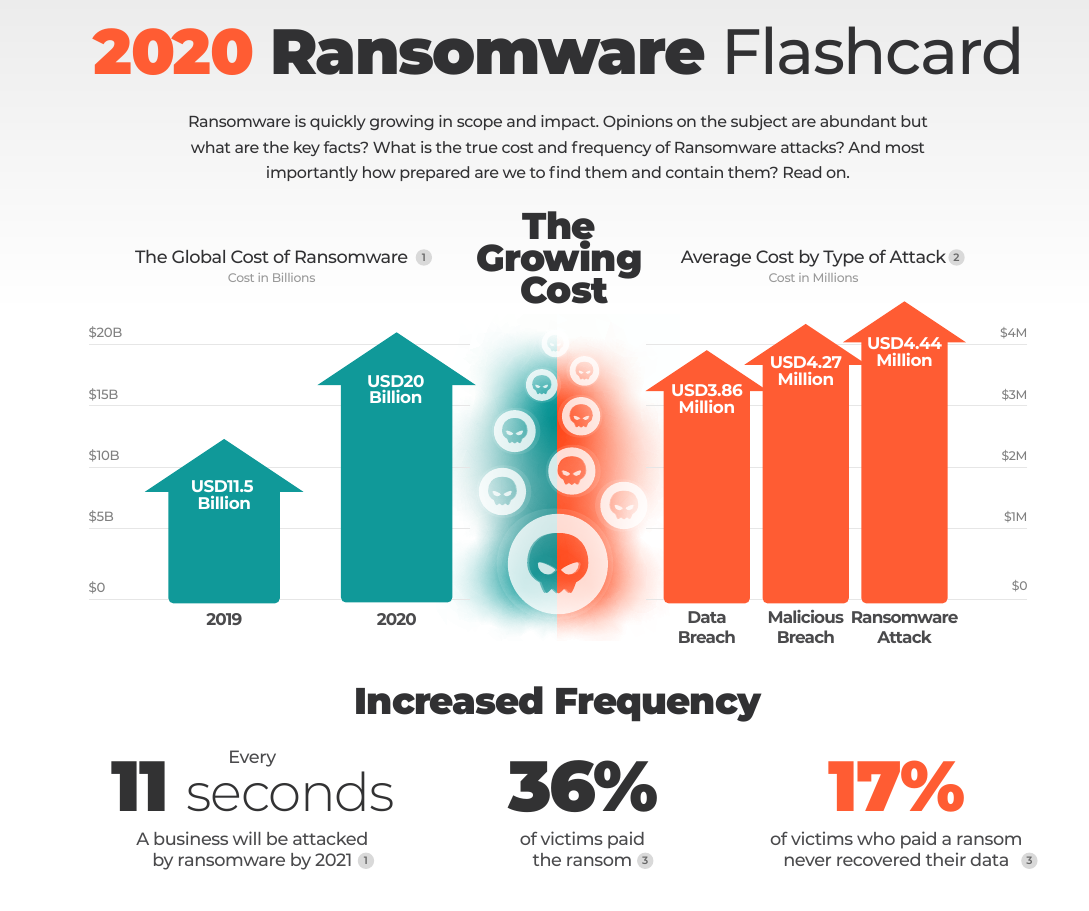
\includegraphics[width=0.8\textwidth]{imagenes/ransomware1.png}
  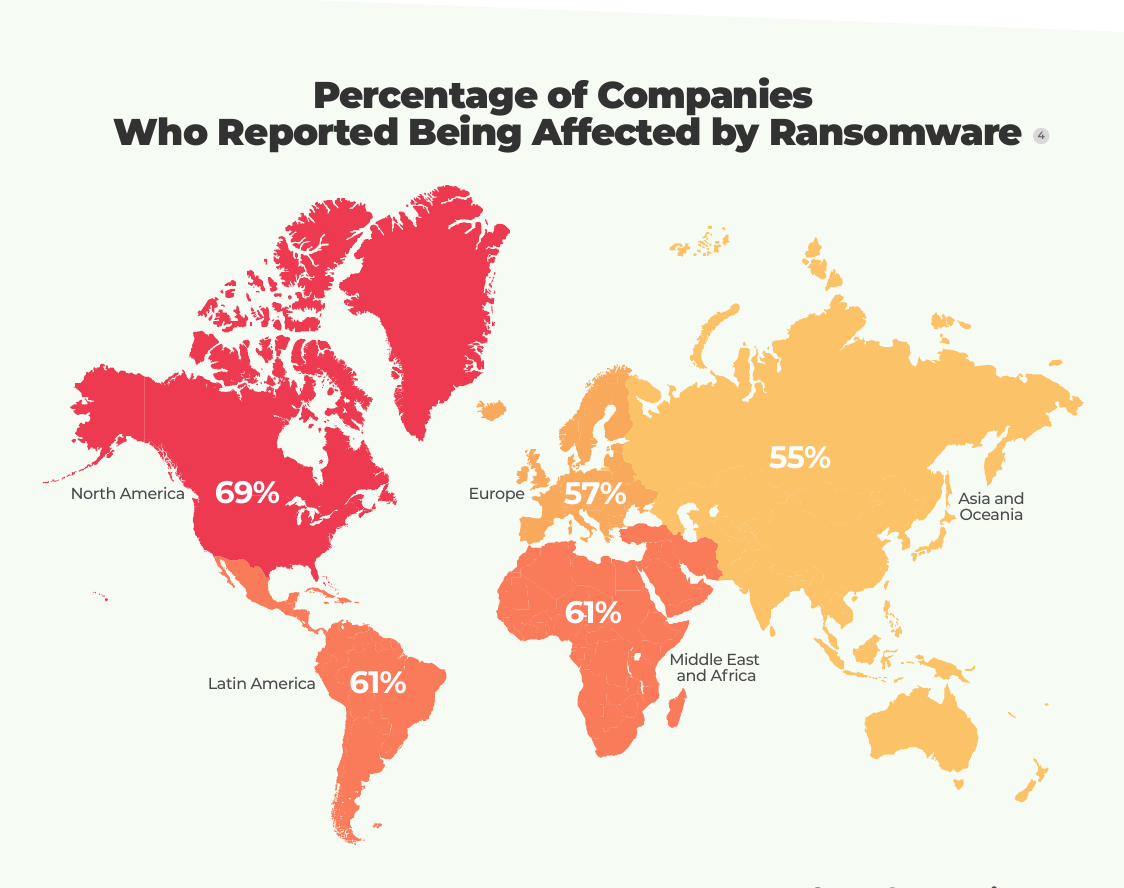
\includegraphics[width=0.8\textwidth]{imagenes/ransomware2.png}  
  \caption{Gráficos extraídos del informe citado del CNN en el que se muestran algunas tendencias de las incidencias relacionadas con \gls{Ransomware} \cite{cnncert}}
\end{figure}


Entre todas estas herramientas aparece \textbf{\textit{Wazuh}}\footnote{Ver \url{https://wazuh.com/}\cite{WAZUH}}, una plataforma \gls{OpenSource} de ciberseguridad que pretende convertirse en un estándar y una referencia a la hora de proteger los dispositivos informáticos y que engloba distintos tipos de módulos o herramientas que ofrecen, entre otras cosas, recolección y análisis de los registros (\textit{logs}) de los \textit{endpoints} \footnote{Un endpoint es cualquier dispositivo remoto conectado a una red y que genera tráfico de datos: un ordenador portátil, una teléfono móvil, un servidor o incluso un dispositivo IOT}, detección de vulnerabilidades en el software instalado, control de la integridad de archivos sensibles o detección de intrusiones (HIDS).


Wazuh es una herramienta que permite recopilar y analizar información sobre eventos de ciberseguridad que tienen lugar en los sistemas de una organización y alertar a sus responsables cuando dichos eventos tengan una importancia determinada. Sin embargo, esta monitorización requiere de una configuración y puesta a punto previa y no siempre se cumplen los requisitos para \textbf{analizar todas las posibles amenazas}. Si no se trata de sobrepasar las defensas de un sistema, difícilmente se puede saber cómo de seguras son estas. Esta es la razón por la que existen los llamados \textbf{Hackers éticos} y sus \textbf{test de penetración de sistemas}, de los que hablaremos a continuación. En este proyecto se va a analizar el uso de Wazuh (se analizará más adelante su estructura y funcionamiento) y la relación que tienen (o que pueden tener) este software y el \textbf{Hacking ético}.

\begin{figure}[hbtp]
  \centering
  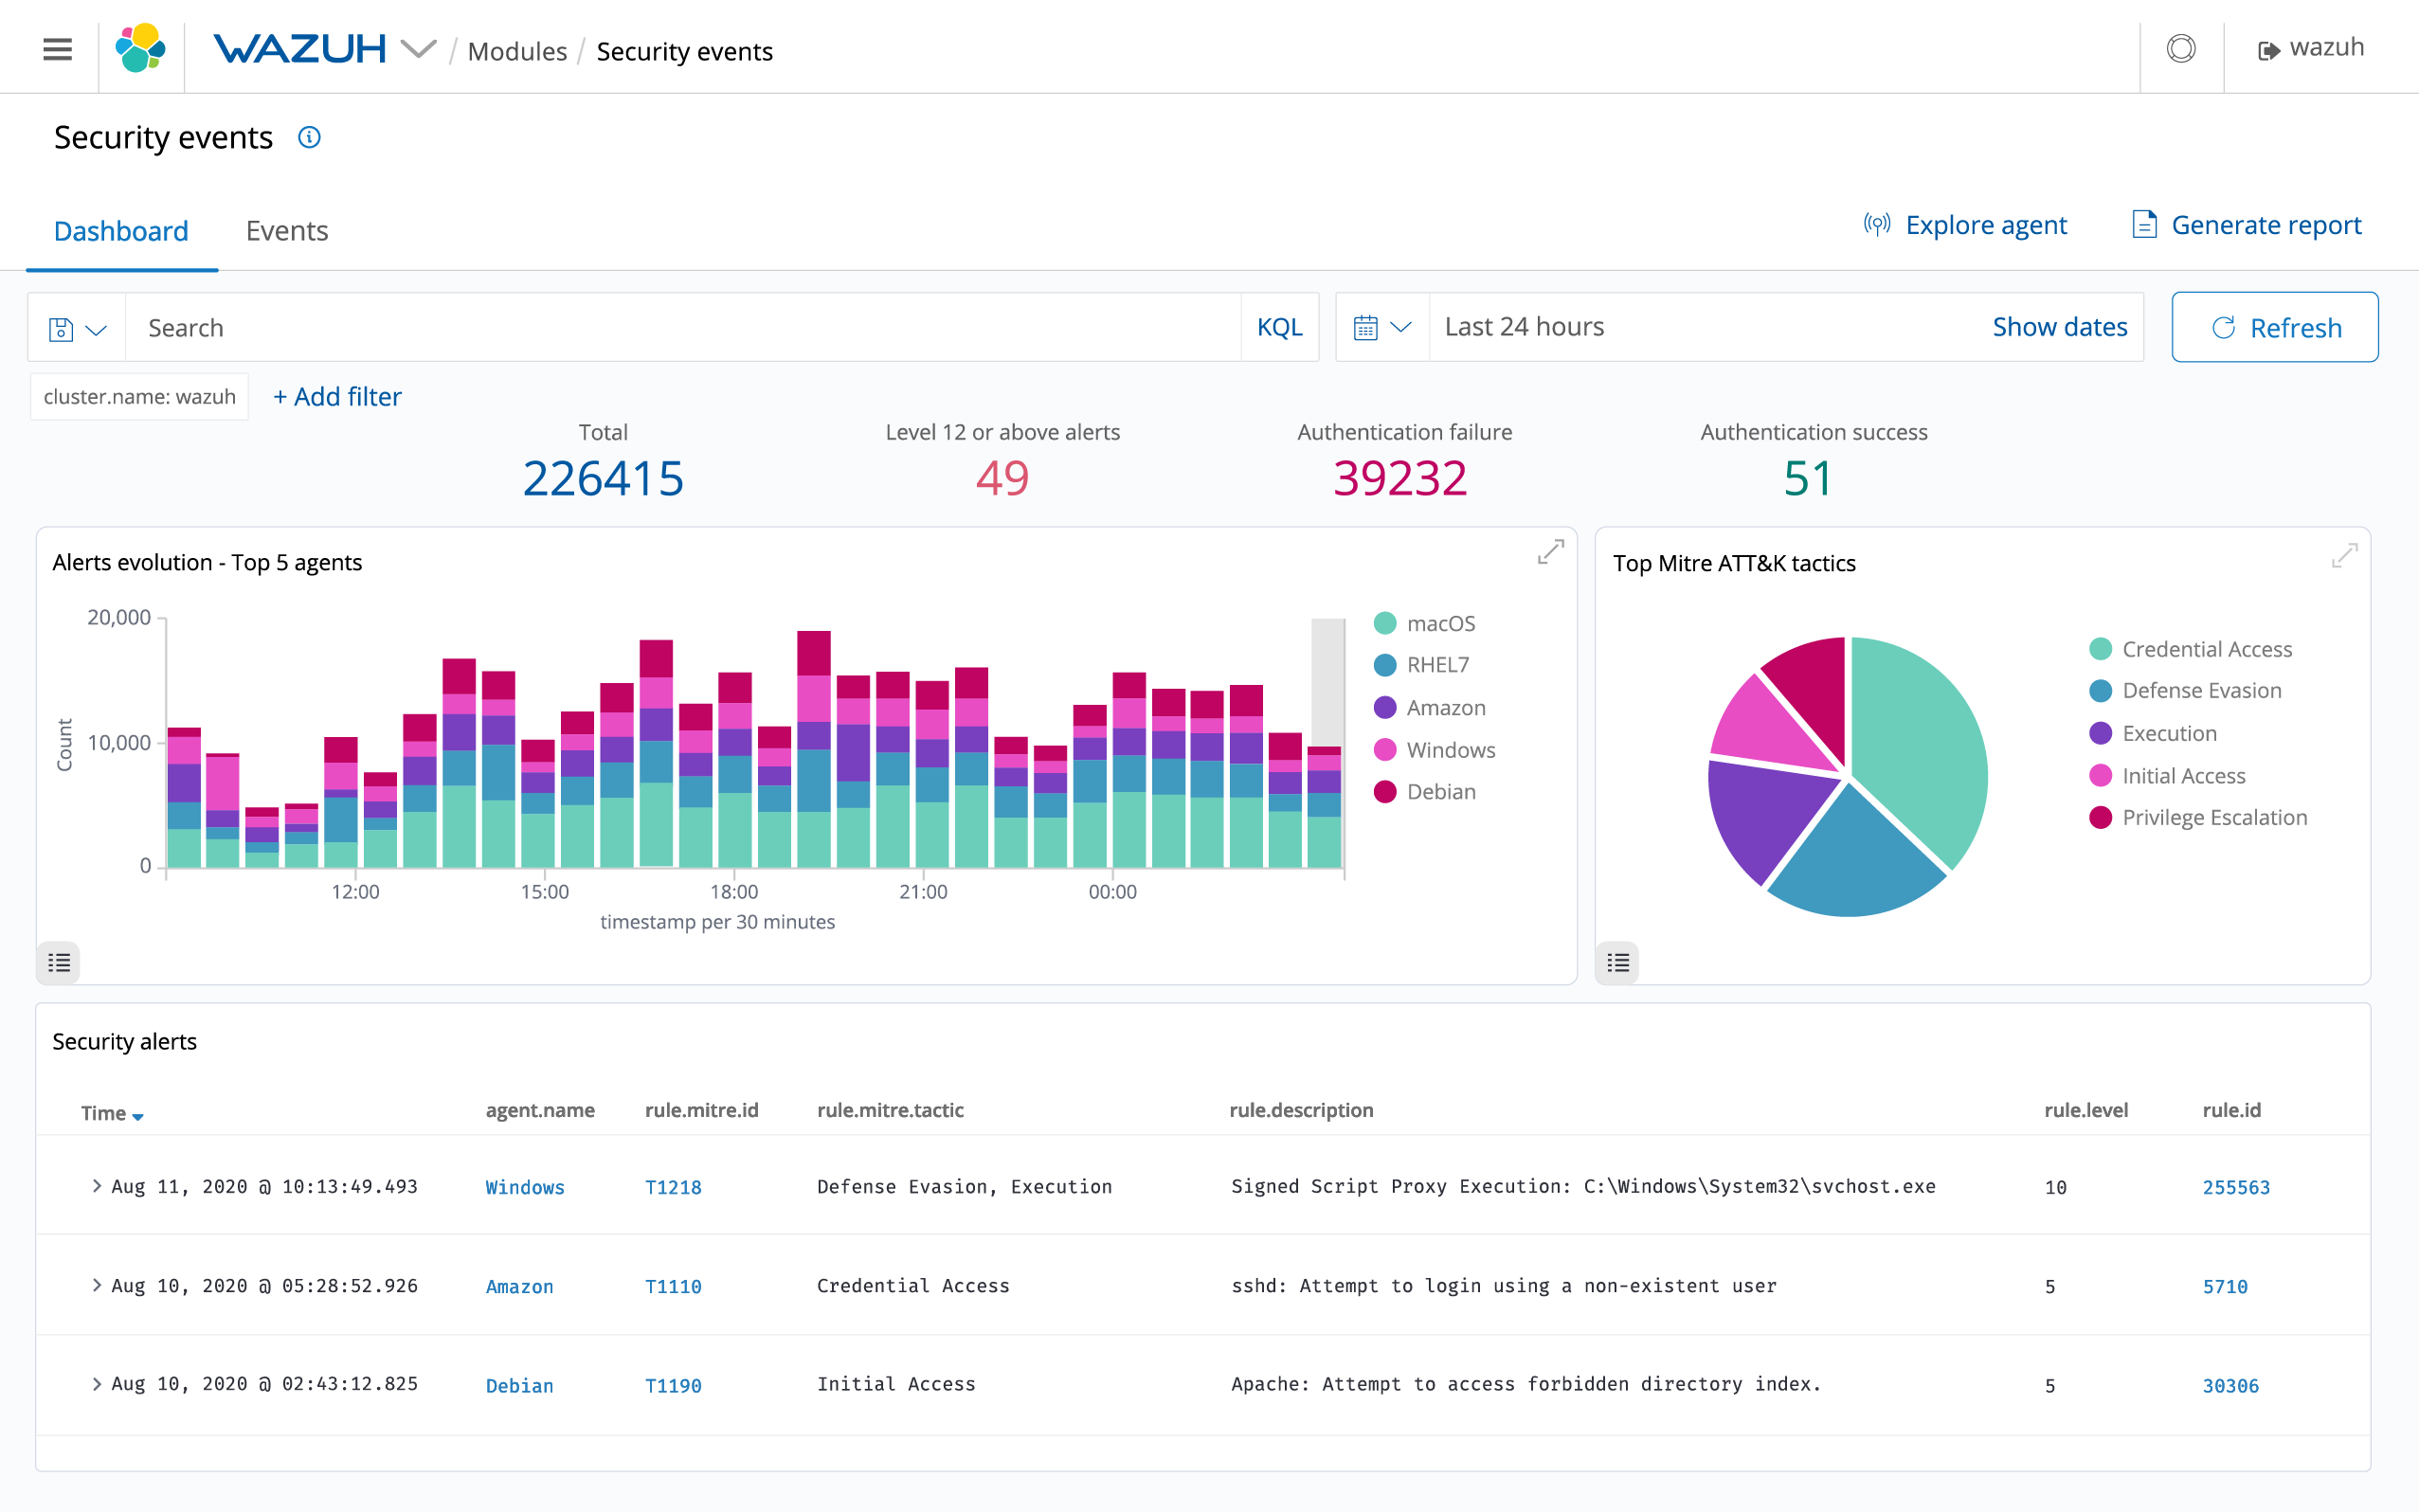
\includegraphics[width=0.8\textwidth]{imagenes/wazuh_kibana.png}
  \caption{Ejemplo de visualización de la interfaz web de Wazuh en la pestaña de `eventos de seguridad'. En ella se aprecian algunas estadísticas de alertas generadas en los sistemas monitorizados.}
\end{figure}

\subsection{\textit{Hacking} ético y seguridad ofensiva}

Un hacker ético es una persona con conocimientos técnicos suficientes que emplea sus habilidades en un marco legal y con fines éticos. Normalmente, son contratados por empresas y cuentan con permiso explícito de la misma para tratar de ganar acceso de forma `ilícita' a los sistemas y a la información de la misma, poniendo a prueba la seguridad de su entorno y realizando un informe o reporte con las conclusiones extraídas. Existen principalmente dos roles que se enmarcan dentro del hacking ético, los analistas que realizan `tests de penetración de sistemas' y aquellos que participan en los programas de \gls{bugb}.

Hoy en día existen multitud de organizaciones en el ámbito de la ciberseguridad que desarrollan herramientas y comparten recursos para los denominados test de penetración de sistemas, en los que buscan extraer toda la información posible de un servidor por medio de técnicas como el escaneo de puertos, descifrado de contraseñas, análisis de redes (\gls{network sniffing}) o \gls{Reverse engineering}. 

Entre ellas cabría destacar la organización \textbf{Offensive security}\footnote{https://www.offensive-security.com/ \cite{offensive}} que ofrece formación y certificaciones para hackers éticos y es muy conocida por ser la creadora de proyectos como \textbf{Kali Linux}\cite{kalilinux}, una distribución de Linux orientada a tests de penetración de sistemas (como \textbf{Black Arch Linux} o \textbf{Parrot OS}) con diferentes configuraciones y herramientas\cite{tools} por defecto dirigidas a facilitar las tareas de un auditor y por sus certificaciones relacionadas con ciberseguridad, que son altamente apreciadas por la comunidad.

\section{Motivación}

Wazuh engloba diversos módulos y herramientas que se enmarcan dentro de las labores de un analista de ciberseguridad y que permiten detectar amenazas cuando estas ocurran y defender los dispositivos de posibles ataques, así como detectar las intrusiones como parte de un análisis forense (\gls{forensics}).

Es un software \textbf{libre y gratuito (\acrshort{FOSS})} y parte del éxito de la empresa se debe a su fuerte comunidad (Open-Source) y a que se trata de un proyecto moldeable y que se adapta a las cambiantes necesidades del entorno de la ciberseguridad actual. 

Sin embargo, hoy en día son fundamentales para los departamentos de seguridad de las empresas las auditorías de seguridad (o tests de penetración de sistemas) y las búsquedas de errores por cuenta ajena (comúnmente conocidas como \gls{bugb}) en las que se trata de poner a prueba un entorno \textbf{desde un punto de vista externo al mismo}, pudiendo encontrarse a veces vulnerabilidades que escapan al alcance de herramientas como Wazuh.

Además, dado que Wazuh es uno de los elementos que utilizan muchas empresas para defenderse de ataques, es también un \textbf{factor más a analizar durante las auditorías de ciberseguridad} o tests de penetración de sistemas. 

Es por ello que se plantean dos ideas importantes sobre la \textbf{relación entre Wazuh y el hacking ético}.

\begin{itemize}
    \item ¿Qué pueden aportar los tests de penetración o las técnicas de \gls{bugb} a la seguridad de un sistema que ya cuenta con Wazuh?
    \item ¿Que puede aportar Wazuh a aquellos que practican el Hacking ético?
\end{itemize}

\subsection{Relación entre Wazuh y el Hacking ético}

Durante este trabajo se tratará de analizar esta relación entre un software `defensivo' y técnicas `ofensivas' que se utilizan como un adversario para evaluar y conseguir mejorar las medidas defensivas de los entornos. 

Por un lado, un test de penetración de sistemas puede sacar a la luz \textbf{vulnerabilidades o defectos}\cite{owasp} del sistema que \textbf{quizá hayan pasado por alto a los mecanismos del software defensivo} (puesto que un software defensivo no siempre puede detectar todos los eventos de seguridad que ocurren en el sistema). De esta forma, el test serviría también para \textbf{evaluar el rendimiento} de la herramienta defensiva (Wazuh, para el caso que nos ocupa) y \textbf{detectar posibles mejoras para el mismo}, ya sea por medio de nuevos módulos o mejorar en los existentes, o porque una escasa configuración de la herramienta la haya hecho ineficiente en un caso concreto y se requieran cambios en la misma.

Por otro lado, \textbf{Wazuh puede responder a una necesidad importante en el ámbito del hacking ético}, en el que la \textbf{recopilación y el almacenamiento} de la información extraída de los dispositivos analizados muchas veces se realiza en ficheros de texto plano y sin un formato específico, lo que \textbf{hace difícil su análisis y distribución}. Wazuh cuenta con bases de datos internas y un motor de alertas que se integra con Elasticsearch, y tiene su propia interfaz web con visualizaciones de datos y varios motores de análisis de información de seguridad. Si se pudiera enviar la información de los test de penetración (o similares) a Wazuh para que fuera analizada, decodificada e indexada en un motor de búsqueda como es Elasticsearch, \textbf{se estaría supliendo una de las necesidades más básicas de cualquier hacker ético}. Además, dentro de la comunidad de hacking ético se anima a \textbf{tratar de automatizar todos los procesos que se pueda}, especialmente la recopilación y análisis inicial de información de los sistemas (por ejemplo en la charla que citamos de \cite{hakluke}\footnote{Ver \cite{hakluke}, How to Crush Bug Bounties in the first 12 Months} que habla sobre cómo prosperar en el mundo del Bug Bounty), y Wazuh podría ser un elemento clave para construir herramientas que permitan llevar esto a cabo.

Es por esto que consideramos muy importante comenzar a crear y/o mejorar la interacción entre el mundo del hacking ético y la comunidad de herramientas `defensivas' como Wazuh. 

\subsection{Oportunidad de negocio}

Además, dado que Wazuh es completamente gratuito. Los ingresos de la compañía no dependen de `ventas' de licencias o similares sino de otros \textbf{servicios como el soporte técnico o la \gls{cloud}} \cite{wcloud} de Wazuh. 

Dado que Wazuh es una herramienta altamente configurable, una mala (o insuficiente) configuración del software o la escasa formación de sus usuarios puede causar que queden partes del sistema, que podrían ser analizadas, sin monitorizar, o que eventos que Wazuh ha sido capaz de detectar no sean atendidos o no se tomen las medidas requeridas a tiempo.

Un aspecto interesante por tanto a valorar es la \textbf{oportunidad de negocio} que supondría integrar tests de penetración de sistemas junto con los servicios de soporte técnico que fueran \textbf{especializados} en comprobar y confirmar que Wazuh está correctamente configurado para analizar todos los puntos de interés de los distintos dispositivos de la empresa, así como de confirmar que los empleados y encargados de mantener los sistemas seguros sepan hacer un buen uso del software.  

De esta forma, utilizando conocimientos sobre hacking ético, cualquiera con conocimientos sobre el software de Wazuh podría ofrecer un servicio específico de auditoría de sistemas que incluya un test de penetración junto con la instalación o configuración de Wazuh. Analizando qué puntos está cubriendo el software y cuales podría cubrir con la configuración adecuada o por medio de mejoras en el mismo.

Para la compañía detrás de Wazuh, esta sería una oportunidad de generar \textbf{valor añadido} a sus ya existentes servicios (como el de soporte técnico) o incluso añadir nuevos servicios, basados en la seguridad ofensiva, para \textbf{afianzar clientes} o conseguir otros nuevos.

\section{Justificación y objetivos}

El objetivo de este trabajo es, por tanto, analizar la relación entre un software defensivo como Wazuh con aquellas técnicas y herramientas propias del hacking ético. Responder a las preguntas planteadas:

\begin{itemize}
    \item ¿Qué pueden aportar las técnicas de hacking ético a Wazuh?
    \item ¿Qué puede aporta Wazuh a los hackers éticos?
    \item ¿Cómo pueden relacionarse estos sistemas entre sí?
\end{itemize}

En primer lugar, y dado que consideramos que herramientas más complejas (como es el caso de Burp Suite, ver \cite{burp}) tienen su propio mecanismo de registros que pueden ser enviados a Wazuh y analizados con cierta facilidad, se propondrán y estudiarán distintos medios para \textbf{registrar los resultados de la ejecución de herramientas en consola de comandos} (como, por ejemplo, nmap, aircrack o Nikto), se evaluará la viabilidad de cada método y la posibilidad de integrarlos con Wazuh para indexar la información generada por estos.

Una vez hecho esto, se evaluará el rendimiento de Wazuh en un escenario que simule la realidad, instalándolo en una máquina vulnerable y sometiendo a esta a un test de penetración. La idea es detectar cómo puede Wazuh servir para detectar cierto tipo de ataques y cómo se podría mejorar la herramienta. De esta forma, se valorará la utilidad de emplear las técnicas de penetración de sistemas \textbf{para evaluar el rendimiento de Wazuh como herramienta defensiva}.

Por otro lado, evaluaremos qué se puede detectar (generar alertas o notificaciones ante eventos de importancia) usando el módulo desarrollado. Se estudiará cómo puede esto \textbf{complementar a la labor defensiva de Wazuh} y la correlación existente entre los eventos detectados por Wazuh (con sus módulos por defecto) y aquellos detectados usando la herramienta desarrollada. Es decir, revisaremos si la herramienta complementa a Wazuh, notificando de eventos que este pasa por alto o si sirve más bien para verificar desde otra perspectiva que Wazuh esté detectando los eventos correctamente.

En resumen, los objetivos principales del proyecto son:

\begin{itemize}
    \item Crear una herramienta que sirva de nexo entre Wazuh y las herramientas típicas de pentesting.
    \item Evaluar el aporte de las técnicas de hacking ético a la herramienta de Wazuh.
    \item Estudiar el valor que ofrece Wazuh a los hacker éticos en sus actividades.
\end{itemize}


\section{Estado del arte}\label{sec:estado del arte}

Existen diversas herramientas para el registro de eventos en los diferentes sistemas operativos, sin embargo, a día de hoy, no hay variedad en cuanto a herramientas que estén especializadas en recopilar o analizar los registros o las salidas generadas por herramientas propias de una auditoría de ciberseguridad y, en general, las opciones que existen están limitadas por uno u otro lado.

Las distintas soluciones y herramientas que existen para monitorizar o registrar la ejecución de comandos en una consola serán descritas posteriormente en el \autoref{cap:Registro}, si bien no ahondaremos más en ellas en esta sección sí que mencionaremos una herramienta existente cuyo propósito es bastante similar al que se define en este proyecto.

\subsection{Faraday: un entorno colaborativo de penetración de sistemas y administración de vulnerabilidades}

\begin{figure}[!hbt]
  \centering
  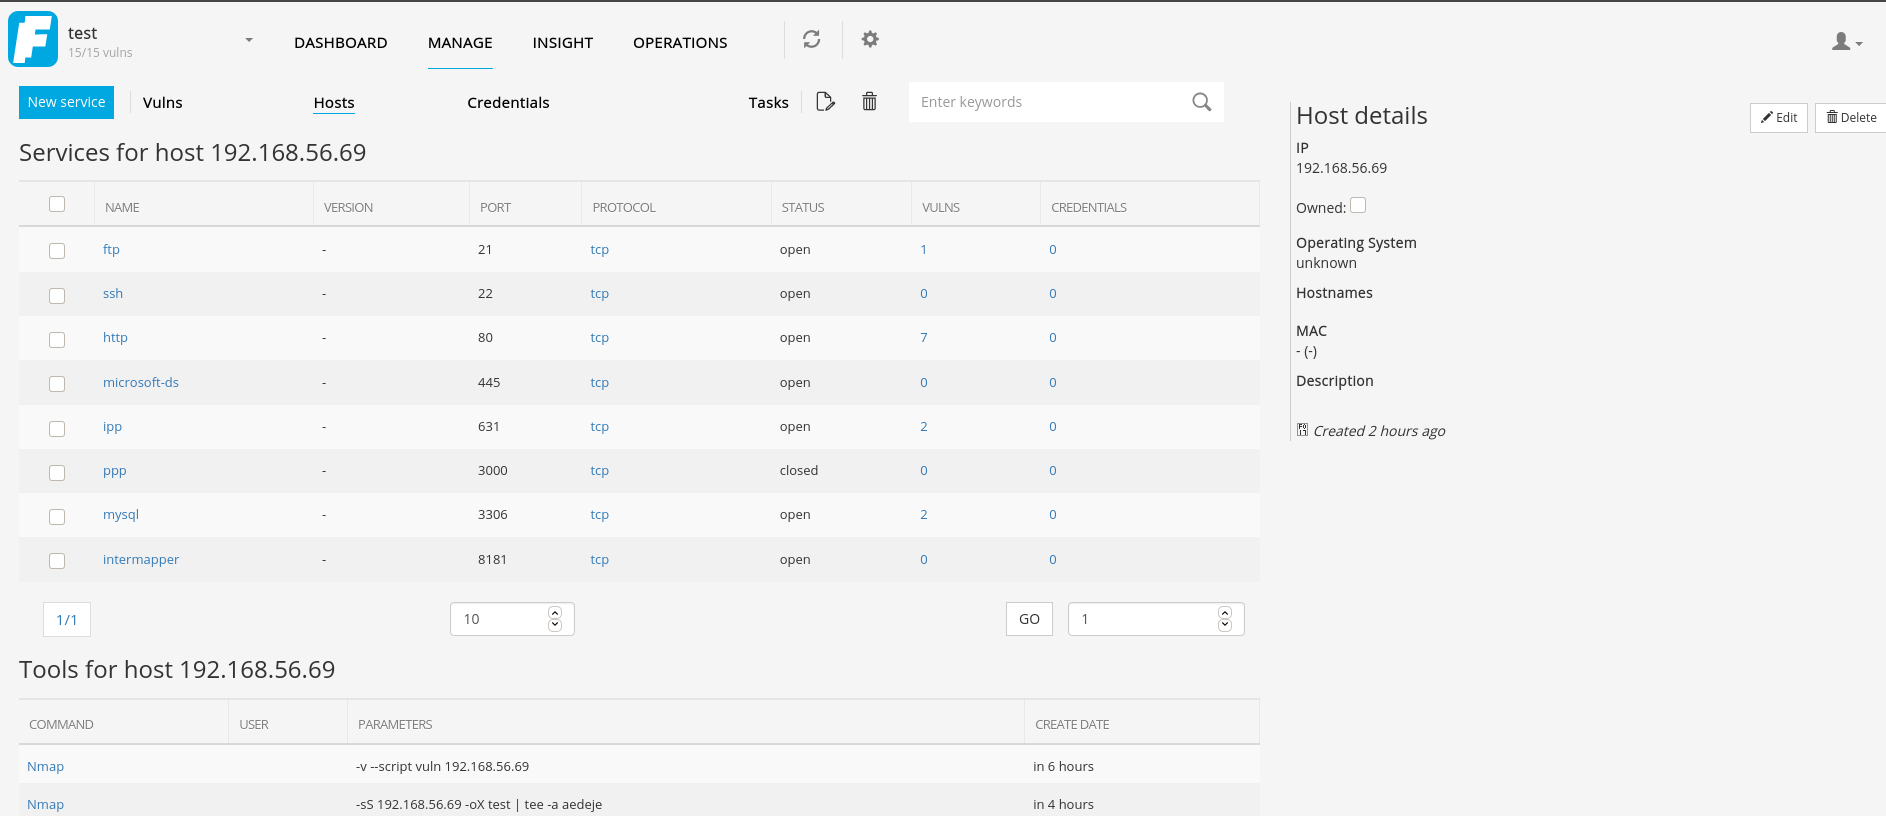
\includegraphics[width=\textwidth]{imagenes/faraday_host.png}
  \caption{Ejemplo de la ventana de hosts con la información extraída por Faraday usando nmap. Fuente: elaboración propia.}
  \label{faraday1}
\end{figure}

\begin{figure}[!hbt]
  \centering
  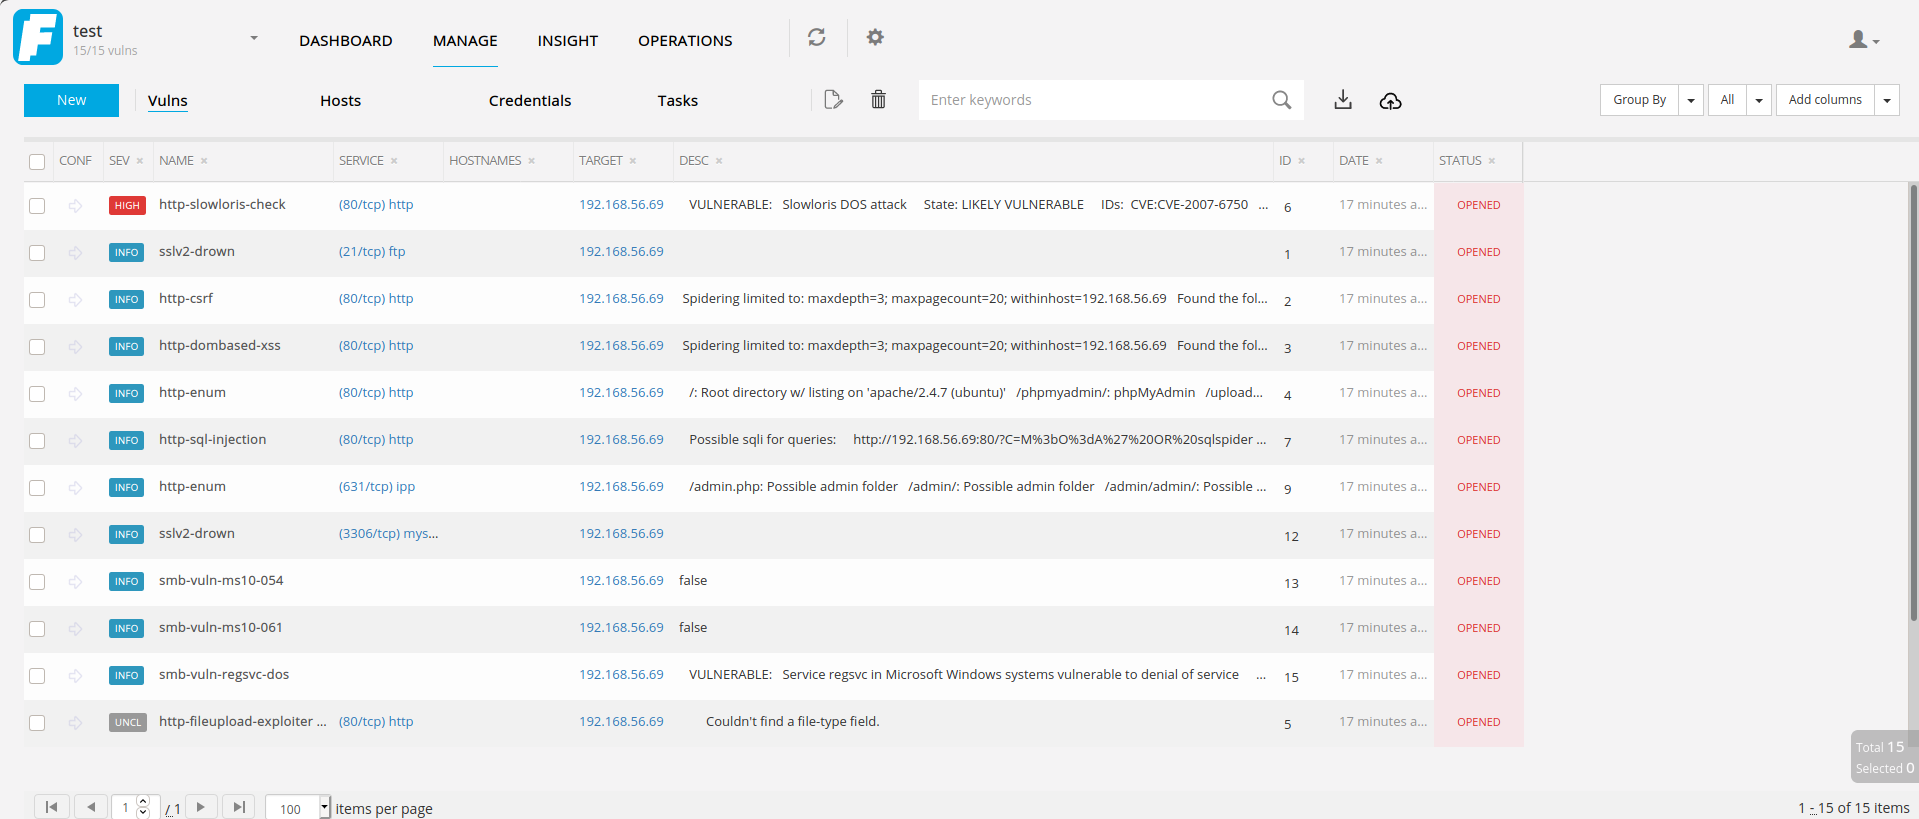
\includegraphics[width=\textwidth]{imagenes/faraday_vuln.png}
  \caption{Ejemplo de la ventana de vulnerabilidades de Faraday. Podemos visualizar las vulnerabilidades localizadas hasta el momento, su importancia. Fuente: elaboración propia.}
  \label{faraday2}
\end{figure}

\textbf{Faraday}\footnote{Ver \url{https://github.com/infobyte/faraday}} es un proyecto que pretende ofrecer una experiencia multiusuario de entorno de desarrollo para test de penetración de sistemas. Está diseñado para analizar datos extraídos de distintas herramientas de ciberseguridad e indexar los resultados del análisis de forma que tengan un formato analizable y fácil de compartir.

\subsubsection{Análisis de Faraday}

Faraday es un producto bastante nuevo, su primera \textit{release} disponible en Github data de finales de 2019 y tiene un soporte bastante activo en la actualidad. De hecho, es una de las herramientas que vienen por defecto en la distribución de Linux destinada a pentesting: Kali Linux.

Dispone de un servidor principal y varios clientes que se le conectan. El servidor utiliza un backend con una base de datos relacional postgreSQL. 

\begin{figure}
\begin{lstlisting}[language=bash,caption={Ejemplos de transformaciones de código hechas por Faraday}]
[1] sudo nmap -sS 192.168.56.69
[1] sudo nmap -oX /tmp/Nmap_04cgvggq.xml -sS 192.168.56.69 2>&1 | tee -a tmp.MCqWwd589v0Lk6l0bThFlEsrXWkhQ 

[2] sudo nmap -sS -oX test 192.168.56.69  | tee -a test_2
[2] sudo nmap -sS 192.168.56.69 -oX /tmp/Nmap_tuuvu2vm.xml | tee -a aedeje 2>&1 | tee -a tmp.qulP2E4IPQVgGzteTTQilsSOoe74c
\end{lstlisting}
\caption{Ejemplo de cómo transforma Faraday los comandos introducidos.}
\label{farday_transformation}
\end{figure}


Un primer detalle que llama la atención de su cliente es que dispone de una consola propia de comandos, integrada en una aplicación de escritorio y que modifica los comandos introducidos, como se aprecia en la figura \ref{farday_transformation}. Faraday fuerza a nmap a generar un output en xml en el directorio tmp y a enviar el output del comando a otro fichero en tmp [1]. De hecho, si se le pide a nmap que genere un archivo de output específico (test) [2], Faraday quitará esa opción y la sustituirá por la que tiene por defecto. Si enlazamos la ejecución de nmap con el comando `tee', Faraday no modificará esta acción pero si la encadenará con otra ejecución de `tee' para escribir en otro archivo temporal. 


Una vez escaneado un servidor en Faraday (usando, por ejemplo, nmap), dispondremos de una ventana específica para dicho host dentro del servidor (accesible a través de una aplicación web) tal y como se aprecia en las figuras \ref{faraday1} y \ref{faraday2}. Ahí encontramos información sobre puertos abiertos, servicios y versiones de los mismos. Sería muy interesante que Wazuh contara con una base de datos similar y visualizaciones en su app, y que se pudiera rellenar dicha base de datos con la información extraída por medio de técnicas de pentesting.

Así mismo, en Faraday también se almacenan las vulnerabilidades detectadas en los hosts analizados, junto con alguna información de interés, y cuenta con medios y plantillas para ayudar a crear \textbf{reportes de calidad} (característica que comparte con Wazuh).

Cabe señalar que Faraday se centra en registrar vulnerabilidades y servicios de los hosts, pero, sin embargo, no registra el output de los comandos ejecutados una vez los ha analizado. 

Es una herramienta muy interesante e investigarla nos ha servido para entender mejor qué tipos de proyectos existen para facilitar las labores de un pentester, si bien no hemos encontrado muchos documentos o testimonios de gente que utilice la herramienta en su trabajo, aunque en la web oficial del producto se mencionan a diversas compañías que la utilizan.

El análisis de esta herramienta nos brinda una idea general de a qué podría aspirar un proyecto basado en Wazuh cuyo objetivo sea \textbf{complementar los test de penetración de sistemas} y ofrecer una forma fácil de almacenar e indexar información generada durante la auditoría.

Analizaremos en puntos posteriores como podemos llevar esto a cabo.



\section{Planificación}

El trabajo se dividirá en cuatro fases: 

\begin{itemize}
    \item Una primera fase de investigación y análisis de los fundamentos teóricos en la que se definan los conceptos clave para el desarrollo del proyecto. Se desarrollará principalmente durante las primeras semanas del trabajo y los resultados se enmarcarán en el Capítulo \ref{cap:Fundamentos}
    \item Una segunda fase en la que se dedicará algo de tiempo a poner a punto algunos entornos de pruebas. Desplegar e instalar máquinas virtuales y provisionarlas con Wazuh y cualquier herramienta que hiciera falta.
    \item Una tercera fase, que será el grueso del proyecto y en la que se analizará el problema de capturar la ejecución de comandos en una terminal, se propondrán soluciones y se valorarán las más convenientes. Además, en esta fase se desarrollará una herramienta para capturar y enviar comandos a Wazuh, así como algunas reglas y decoders de ejemplo. 
    \item Finalmente, en la cuarta y última fase del proyecto se estudiará un caso de uso práctico y se analizará la aplicación de la solución desarrollada en la fase anterior en un entorno real, así como la viabilidad de enfocar un test de penetración de sistemas a la evaluación del uso de Wazuh o de utilizar Wazuh como un complemento para las labores de un hacker ético.
\end{itemize}

\subsection{Distribución de horas dedicadas al proyecto}


Para controlar el tiempo dedicado al proyecto (un trabajo de fin de grado debe rondas las 300 horas de trabajo), se utilizará \textbf{Clockify}\footnote{https://clockify.me}, una herramienta que permite tomar medidas de tiempo durante el que se está trabajado y etiquetarlas según la fase del proyecto en la que se esté añadiendo esfuerzo.

El número total de horas dedicadas por fase en los años 2020 y 2021 está reflejado en las figura \ref{clockify_horas} y las fases definidas, en la figura \cite{clockifyfases}, aunque obviamente se han dedicado más horas al trabajo que por distintas razones pueden no haber sido registradas usando esta aplicación.%, por no hablar de las horas laborales trabajando como ingeniero en Wazuh en las que he acabado trabajando en algo a raíz del estudio realizado para este proyecto. 


\begin{figure}[!hbt]
  \centering
  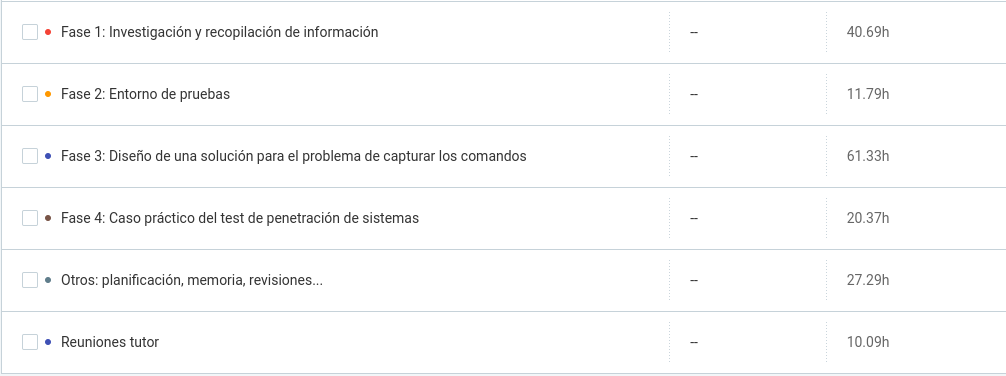
\includegraphics[width=\textwidth]{imagenes/Fases.png}
  \caption{Captura de pantalla del menú de \textbf{Clockify} dónde se aprecian las fases definidas y las horas dedicadas a cada una de ellas.}
  \label{clockifyfases}
\end{figure}


\begin{figure}[!hbt]
  \centering
  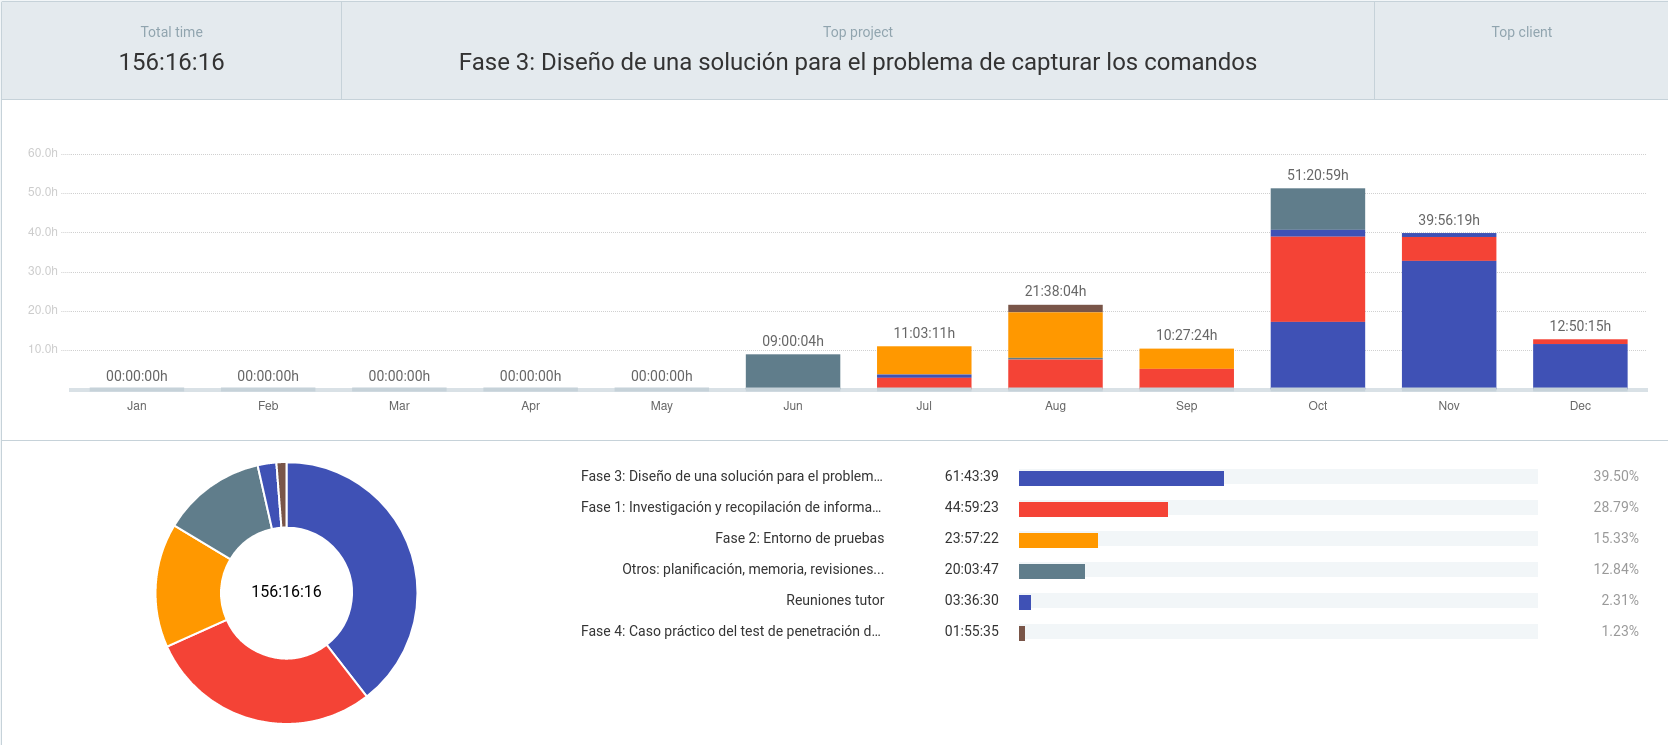
\includegraphics[width=\textwidth]{imagenes/clockifyme_1.png}
  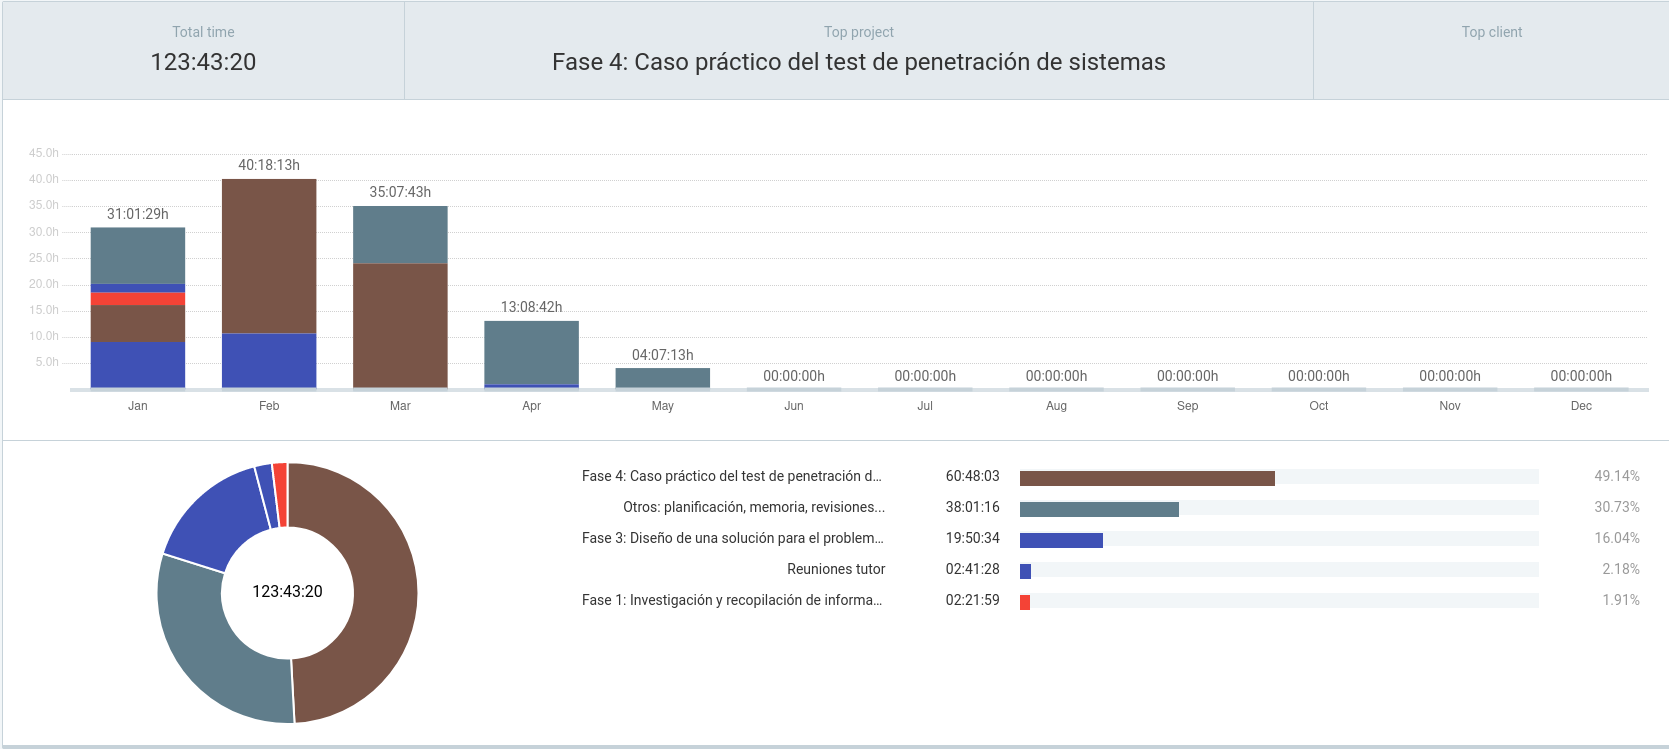
\includegraphics[width=\textwidth]{imagenes/clockifyme_2.png}
  \caption{Distribución de las horas dedicadas al proyecto por fases y por meses (durante 2020 y 2021)}
  \label{clockify_horas}
\end{figure}

\begin{figure}[!hbt]
  \centering
  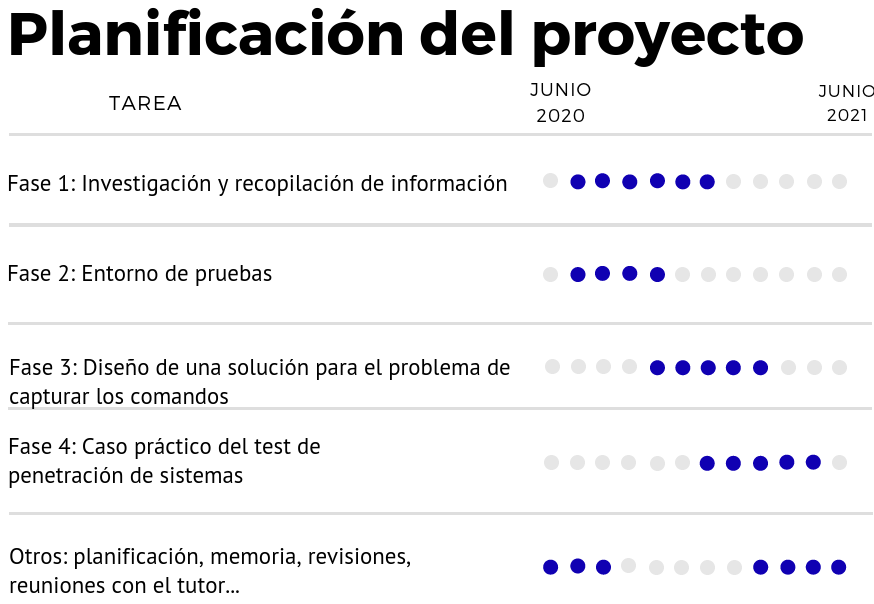
\includegraphics[width=\textwidth]{imagenes/gantt.png}
  \caption{Diagrama de Gantt con una estimación de la distribución del tiempo dedicado a cada fase de proyecto por meses (entre los meses de Junio de dos mil veinte y dos mil veintiuno. Cada punto representa un mes. Debemos tener en consideración que esta es una planificación global del proyecto, por meses y no por horas, y que la distribución de horas al mismo podría variar según el mes. Además, el hecho de que algunas fases se solapen se debe a que dependen unas de horas y es probable que haga falta dedicar tiempo de forma concurrente a varias fases a la vez. Por último, señalar que al apartado `otros' se le han marcados los meses iniciales y finales del trabajo por el esfuerzo extra que requiere la puesta en marcha del mismo y la entrega final, pero se anotará todo el tiempo dedicado a otros quehaceres fuera de las fases ya definidas y se englobará en este grupo. A la hora de crear este y otros gráficos se han tenido en cuenta las direcciones expuestas en el Capítulo 5 de  \cite{books/daglib/0076234}.}
  \label{gantt}
\end{figure}

La planificación de las horas dedicadas a cada fase se ha hecho siguiendo el diagrama de Gantt que se describe en la figura \ref{gantt}.








\section{Estimación de presupuesto}

Para finalizar la introducción del proyecto, sería interesante hacer una estimación del coste que podría haber tenido para una organización como Wazuh llevar a cabo la investigación y los desarrollos que se han dado en este proyecto. 

Se estima que se han invertido más de 300 horas (sumando la planificación, reuniones, revisiones y demás), y, dado que existe una alta posibilidad de que las personas que pudieran trabajar en una investigación como esta \textbf{no contaran con la formación previa y los conocimientos necesarios sobre hacking ético} (puesto que esto no es un requisito para trabajar como desarrollador en Wazuh), podríamos estimar que llevar a cabo un proyecto de investigación de esta índole llevaría a la empresa a dedicar a varios ingenieros, que además habrían de ser formados en la materia pertinente durante al menos unos tres meses. Además de los costes asociados a entornos de prueba en la nube y similares.

Si además se quisiera planear un desarrollo formal (más allá de la prueba de concepto que en este proyecto se plantea) que se programara en C y se integrara como parte del proyecto, el número de horas requeridas se dispararía, al igual que el número de equipos involucrados y el tiempo para llevarlo a cabo.

Por hacer una pequeña simulación, suponiendo que se emplean a tres ingenieros sin conocimientos previos sobre hacking ético y que estos deben formarse y se deben pagar algunos laboratorios para hacer pruebas, además de sus sueldos tendríamos una estimación como la de la Tabla \ref{tab:my-table}.

\begin{table}[hbt]
\begin{tabular}{|l|cccc|}
\hline
Requisito    & Cantidad & Horas/Unidad & precio/hora & Coste \\
\hline
Ingenieros   & 3      & 100             & \euro{10} & \euro{3000} \\
Formación    & 3      & 100             & \euro{1}          & \euro{300} \\
Servicios Nube & 1      & 100             & \euro{1  }         & \euro{100} \\
\hline
Total        & -      & -               & -           & \euro{3500} \\
\hline
\end{tabular}
\caption{Esta tabla plantea un posible escenario en el que una empresa empleara a tres ingenieros para realizar las labores planteadas. Dichos ingenieros tendrían que ser formados en los temas tratados (probablemente) y además requerirían algún tipo de recurso o servicios en la nube para poder realizar sus pruebas. Se ha estimado para los servicios de la nube un precio de un euro por hora basándose en los precios más bajos de recursos disponibles en Amazon Web Service \footnote{https://aws.amazon.com/es/ec2/pricing/on-demand/}.} Además, el precio de la formación se ha estimado en un euro por hora basandonos en la disponibilidad de múltiples cursos (mencionados en la sección \ref{entornos_didacticos}) que con una pequeña suscripción mensual permiten acceder a multitud de contenidos de formación en ciberseguridad, haciendo que el coste de aprendizaje por hora (de forma autónoma, sin un profesor y utilizando los recursos de la plataforma) sea más bajo.
\label{tab:my-table}
\end{table}


\bigskip

\chapter{Fundamentos teóricos para el desarrollo del proyecto}\label{cap:Fundamentos}

En este capítulo, enmarcado dentro de la primera fase de investigación y recopilación de información, enumeraremos aquellos aspectos cruciales para entender el resto del trabajo, que se han estudiado y analizado durante el desarrollo de este trabajo.

\section{Descripción técnica de Wazuh}

Wazuh es una \textbf{plataforma opensource de ciberseguridad}. Esto significa que \textbf{contiene distintos módulos que engloban muchas de las funcionalidades típicas de herramientas de seguridad defensivas}. 

Por ejemplo, Wazuh puede ser utilizado como un \textbf{\gls{siem}}, como un \textbf{\gls{HIDS}}, como una herramienta de monitorización de \textbf{integridad de ficheros}, entre otras funciones.

\begin{figure}[!hbt]
  \centering
  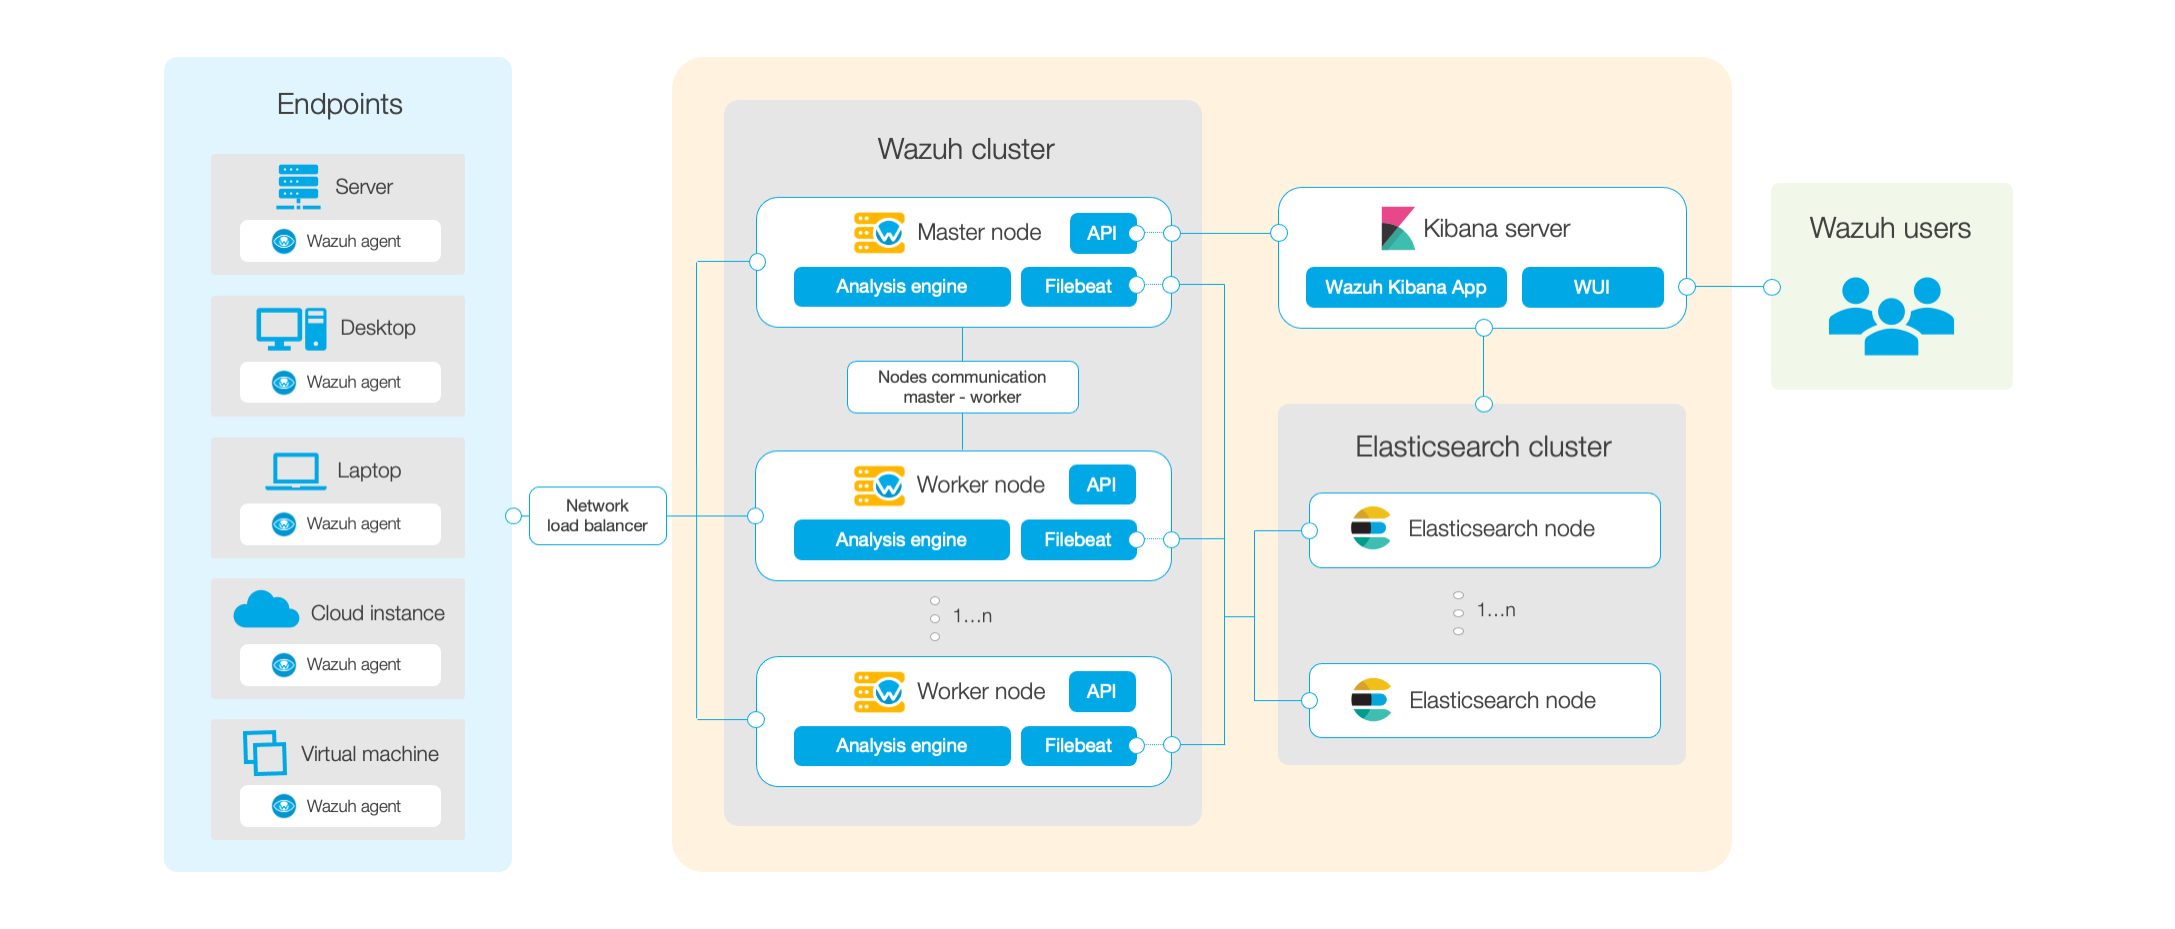
\includegraphics[width=\textwidth]{imagenes/wazuh_architecture.png}
  \caption{Esquema de la arquitectura de funcionamiento completo de Wazuh. Compuesta por uno o varios endpoints (que serán analizados por Wazuh), un cluster de gestores de Wazuh, un cluster de nodos de Elasticsearch y un servicio web Kibana con un plugin específico llamado `Wazuh Kibana App`. }
  \label{wazuh_architecture}
\end{figure}

Para entender mejor cómo funciona, debemos atender a su arquitectura (ver figura \ref{wazuh_architecture}). Wazuh tiene dos elementos esenciales: \textbf{un \textit{manager}, o gestor, y un agente}, que se comunican entre sí. 

El agente de Wazuh se instala en los \textbf{endpoints} o dispositivos informáticos a analizar y se encarga de \textbf{extraer información importante de esos sistemas}, esta extracción de información puede ser por muchas vías \textbf{dependiendo de cómo esté Wazuh configurado}. Por ejemplo, se puede extraer información del propio sistema operativo utilizando el módulo de \textbf{syscollector} o de eventos (borrado, modificación, creación) relacionados con ficheros importantes del sistema con el módulo de \textbf{syscheck o File Integrity Monitoring}, entre otros. Además, los agentes se pueden configurar para leer y redirigir los logs de aquellas aplicaciones que nos sean de interés al gestor, dónde se analizarán como corresponda.

\begin{figure}[!hbt]
  \centering
  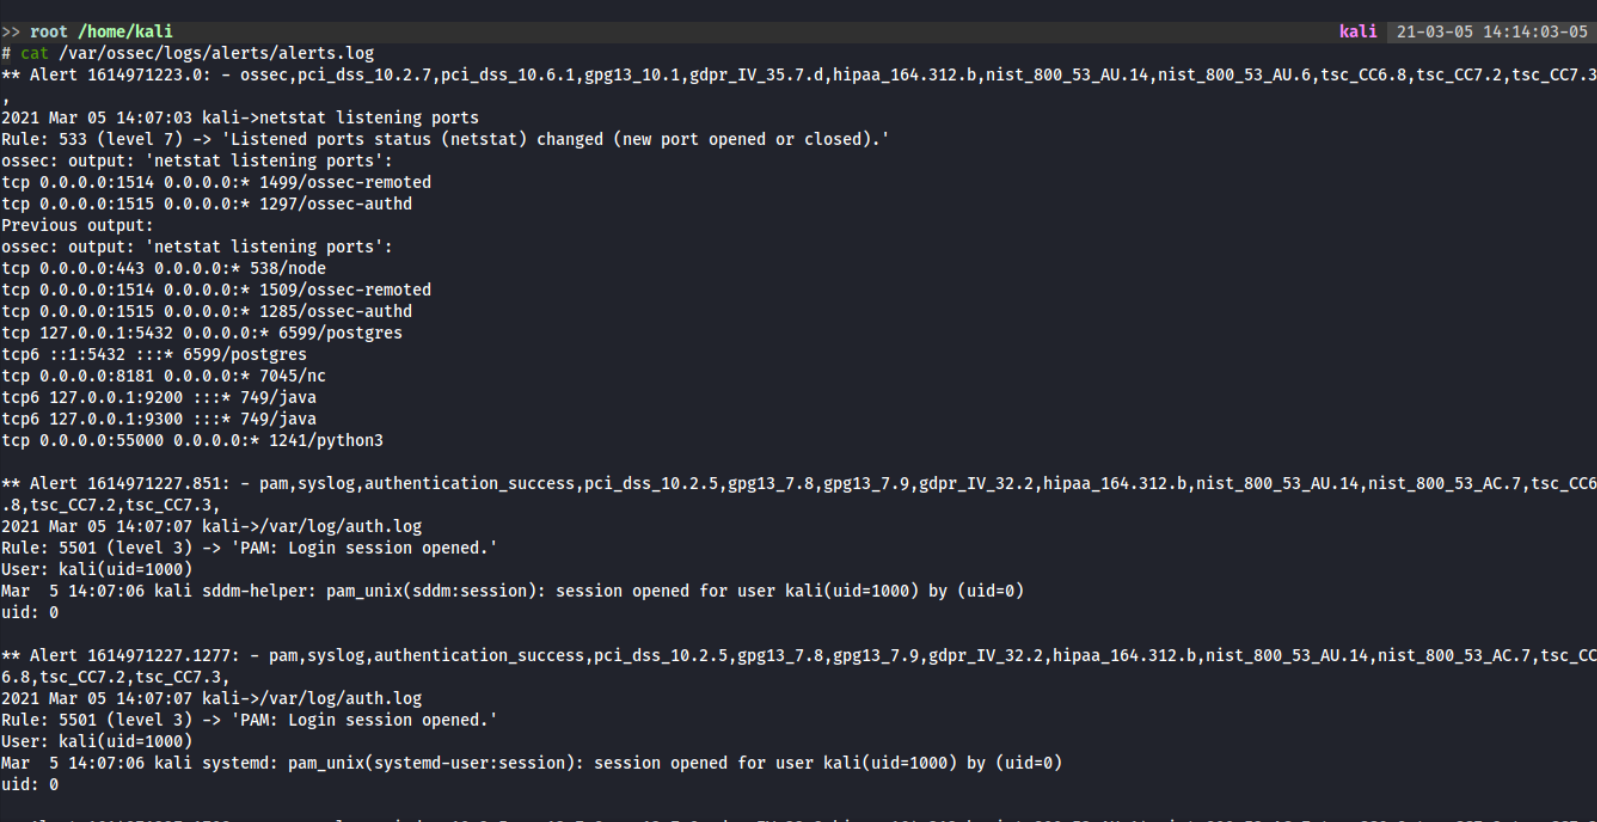
\includegraphics[width=\textwidth]{imagenes/alerts.png}
  \caption{Ejemplo de alertas en texto plano generadas por el gestor de Wazuh a partir de los eventos enviados por los agentes.}
  \label{wazuh_alerts}
\end{figure}


Por su parte, el \textit{Wazuh manager} recibe la información de los agentes. Parte de esta información es almacenada en bases de datos internas (información del OS, paquetes instalados, estados de los ficheros cuya integridad se está asegurando, etc...) y el resto es analizada (principalmente logs) y utilizada para generar \textbf{alertas de seguridad} (ver figura \ref{wazuh_alerts}). 

La información enviada por el agente se considera un \textbf{evento de seguridad} y es decodificada por el gestor para extraer los campos interesantes utilizando \textbf{decodificadores}. A continuación, la información extraída con dichos decodificadores pasa a través de unas \textbf{reglas} que determinan si se trata o no de un evento relevante, así como el tipo de evento, su grado de importancia, si está relacionado con alguna técnica de \gls{mitre}, etc. y ese evento pasa a ser una \textbf{alerta}, que se envía a la aplicación web por medio de Elasticsearch y a aquellos puntos para los que se haya configurado Wazuh (email, SMS, slack, telegram, etc...), esta funcionalidad de alertas con información relevante puede ser de mucho interés para los hackers éticos, como ya se ha explicado.

Es interesante comentar que Wazuh comenzó utilizando Elasticsearch con su versión original, llegando a dar soporte a sus funcionalidades de pago (xpack), pero que en el último año ha comenzado a dar soporte a otra alternativa opensource que ofrece las mismas funciones de forma libre y gratuita (Opendistro).

Con el reciente cambio de licencia en el proyecto de Elasticsearch (\cite{licensechange}), debido en parte a una disputa con Amazon, el entorno de Software que, como Wazuh, utilizan Elasticsearch, se encuentra en un momento inestable. Recientemente, Amazon ha hablado de una versión de Elasticsearch que continúe con la licencia opensource previa, llamada OpenSearch, y mantenida por la propia organización \cite{OpenSearch}. Para este trabajo, se ha mantenido la integración de Wazuh con la versión original de Elasticsearch pero \textbf{es muy probable que en un futuro cercano Wazuh se pueda integrar con otras alternativas}.

Estas reglas y decoders ya mencionados son parte del \textbf{ruleset} de Wazuh, y los usuarios pueden modificarlas o \textbf{crear la suyas propias} para extender la funcionalidad de Wazuh.

Una parte de este trabajo será analizar cómo recopilar datos de la auditoría de seguridad y enviarlos a Wazuh para que los analice como cualquier otro registro con información que llegue al gestor.

Entonces, utilizando la aplicación web de Kibana con \textbf{el plugin de Wazuh}, el usuario puede acceder a estos datos de alertas (así como a los datos disponibles en las bases de datos del gestor, a través de la API de Wazuh, por ejemplo para obtener información sobre los sistemas de los clientes), generar gráficos, tablas y reportes, hacer búsquedas según el valor de determinados parámetros, etc.

El objetivo último de poder generar y analizar información de las auditorías de seguridad con Wazuh sería \textbf{indexar esta información en Elasticsearch} de forma que pudiera ser fácilmente accesible, que se pudieran generar gráficos o reportes a partir de ella, etc.


\section{Definición de hacking ético}

De acuerdo con la guía de estudio del certificado de hacking ético (CEH) \cite{ceh}, un hacker ético (o penetration tester) es aquel que, con permiso explícito de una organización, utiliza sus habilidades como hacker para atacar los sistemas de la misma con el objetivo de descubrir vulnerabilidades. Un hacker ético no revela la información obtenida de dichos ataques a terceros y trabaja siempre con un contrato que garantice actuar dentro de los marcos legales.

Hoy día, también se denomina hacker éticos a aquellos que participan de los programas de \gls{bugb}, de los que ya se ha hablado anteriormente, y que comparen algunas metodologías y características con los tests de penetración de sistemas, pero en esencia son muy diferentes.

Para entender mejor qué es un hacker ético hay que compararlo con su opuesto: aquellos que aprovechan sus conocimientos sobre los sistemas informáticos para realizar actividades ilícitas sobre los sistemas de terceros, explotando sus vulnerabilidades con el objetivo de obtener algún beneficio. Estos individuos cometen delitos informáticos y van en contra de la ley. 

Dado que un hacker ético debe, por definición, actuar dentro del marco legal, es interesante que estudiemos los aspectos legales del hacking ético.

\section{Aspectos legales del hacking ético}

Es de vital importancia tener en cuenta la necesidad de un \textbf{permiso explícito} para realizar o no determinadas acciones en un sistema que no es nuestro.

Un hacker ético nunca debe hacer su trabajo sin permiso explícito de los responsable del sistema que va a probar y, aún teniendo permiso, debe limitar sus pruebas al ámbito que se establezca en el contrato de trabajo. Sobre esto hablaremos más adelante, cuando expliquemos las fases de las que consta un test de penetración de sistemas.

El porqué de estas medidas es que la ley ampara a cualquiera que sea dueño de un sistema informático y la intrusión en este sin permiso está penada en los principales gobiernos del mundo y, en concreto, en España (véase el Artículo 197 bis del Código Penal en España), dónde el acceso ilícito a un sistema de información sin permiso puede ser castigado con pena de presión de seis meses a dos años.

\begin{tcolorbox}[coltitle=blue!50!black,colframe=blue!25,title=Artículo 197 bis]
El que por cualquier medio o procedimiento, vulnerando las medidas de seguridad
establecidas para impedirlo, y sin estar debidamente autorizado, acceda o facilite a otro el
acceso al conjunto o una parte de un sistema de información o se mantenga en él en contra
de la voluntad de quien tenga el legítimo derecho a excluirlo, será castigado con pena de
prisión de seis meses a dos años.

\tcblower

Código Penal y legislación complementaria. Edición actualizada a \linebreak \textbf{17 de diciembre de 2020}
\end{tcolorbox}

\subsection{Convenios internacionales}

Dados que los crímenes relacionados con los sistemas de información pueden ser perpetrados desde cualquier lugar del mundo y, sin embargo, afectar a entidades de otras localizaciones, existen diversos \textbf{convenios internacionales} que indican a los países como proceder en situaciones de esta índole, que un hacker ético \textbf{debe tener en cuenta}, puesto que si se encuentra trabajando para una empresa extranjera podría verse afectado por las leyes de otros países además de las del suyo propio.

\subsubsection{Convenio 185 sobre la ciberdelincuencia}

En este convenio internacional se define el sistema informático como ` todo dispositivo aislado o conjunto de dispositivos interconectados o relacionados entre sí, cuya función, o la de alguno de sus elementos, sea el tratamiento automatizado de datos en ejecución de un programa.', es decir, desde un portátil personal hasta una \textit{smartTV} o un dispositivo \textit{IoT}. Esta definición se corresponde con la de \textbf{endpoint}, que ya hemos mencionado anteriormente y engloba al tipo de dispositivos que pueden ser protegidos por Wazuh.

Del mismo modo, se establecen los delitos contra la confidencialidad, integridad y disponibilidad de los datos y sistemas informáticos y se indica que \textbf{los países participantes deben adoptar las medidas legislativas necesarias para tipificar esos delitos}. Además, la segunda sección del Artículo 12  sobre la Responsabilidad de las personas jurídicas, indica que \textbf{se puede exigir responsabilidad a una persona jurídica cuando la ausencia de vigilancia o control haya propiciado un delito informático}. Todo esto está estrechamente relacionado con el uso de Wazuh en los sistemas que deben ser protegidos o, como se propone en el trabajo, como herramienta para monitorizar las acciones llevadas a cabo durante un test de penetración.

Y es que en cualquier momento un hacker ético puede verse envuelto en conflictos legales si ocurre algún problema durante una auditoría. Así pues, recalcamos la importancia de \textbf{registrar las acciones llevadas a cabo durante la auditoría} puesto que pueden servir como un complemento a la hora de demostrar qué cosas se han hecho o no durante la auditoría.

\begin{tcolorbox}[coltitle=blue!50!black,colframe=blue!25,title=Artículo 197 bis]
 Además de los casos previstos en el párrafo 1 del presente artículo, cada parte
adoptará las medidas necesarias para garantizar que pueda exigirse responsabilidad
a una persona jurídica cuando la ausencia de vigilancia o de control por parte de
cualquier persona física mencionada en el párrafo 1 haya permitido la comisión de un
delito...
\tcblower
Artículo 12 – Responsabilidad de las personas jurídicas del convenio 185 sobre la ciberdelincuencia \cite{t108}
\end{tcolorbox}


\subsection{Leyes y regulaciones a nivel Europeo}

Otro factor clave para entender la importancia de software como Wazuh y el papel que podría tener un especialista analizando el rendimiento de este en un entorno profesional son las regulaciones de seguridad que deben cumplir las empresas.

A nivel europeo existen varias regulaciones que \textbf{las empresas deben cumplir}. Entre ellas, destaca por ejemplo la regulación general de protección de datos (GDPR) que en España se aplica a través del reglamento general de protección de datos (RGPD) \cite{rgpd}, que regula toda la normativa relacionada con la recogida, tratamiento y almacenamiento de datos personales o sensibles como por ejemplo, la información sanitaria de un paciente en un hospital. 
Desde el punto de vista de un analista de ciberseguridad, lo más importante de esta ley son las implicaciones relacionadas con la protección de los datos almacenados. 

En España, basándose en la RGPD, existe la Ley Orgánica de Protección de Datos (LOPD) \cite{lopd}. Tanto la LOPD como la RGPD establecen como se deben tratar los datos personales en nuestros sistemas informáticos, sin embargo, existen unas medidas o normativas extra que las empresas con datos susceptibles de entrar en el marco de estas leyes deben cumplir según el ámbito en el que operen. Son las normativas como HIPAA, PCI DSS o SOC, en inglés comúnmente conocidas como `Compliances'.

Estas normativas se analizarán a continuación, así como sus implicaciones y su relación con software de seguridad como Wazuh.

\section{Normativas de ciberseguridad}

Además de las leyes que establecen los delitos informáticos, existen una serie de regulaciones o normativas propias de los distintos sectores financieros que las empresas que dispongan de determinado tipo de datos deben comprometerse a cumplir. Del inglés \Gls{compliance}, que podría traducirse como 'el cumplimiento' de las normativas o leyes referentes a la seguridad de los datos que una empresa pueda almacenar o gestionar. Cualquier compañía con acceso a datos sensibles de sus clientes está obligada a asegurar unos mínimos requisitos de seguridad en sus entornos y ser capaz de demostrar que los cumple \cite{phoenixnap}. 

Algunos ejemplos importantes de \textit{'compliances'} se enumeran a continuación.

\begin{description}
\item[HIPAA](Health Insurance Portability and Accountability Act) Se aplica a compañías del ámbito sanitario y regulariza cómo dichas compañías deben manejar y asegurar la seguridad de los datos médicos personales de sus pacientes. 

\item[PCI DSS] (Payment Card Industry Data Security Standard) Creado por algunas compañías de la industria de pago con tarjetas de crédito que quiso normalizar como se asegurar la integridad de la información financiera de sus clientes. Wazuh \cite{wazuh-pci} cuenta con herramientas para asegurar este \textit{compliance} asegurando (entre otros) la detección de \textit{rootkits}.

\item[SOC Reports] Se trata de unos reportes de control de sistemas y organizaciones verificable, llevado a cabo por una \acrfull{CPA} para asegurar el cumplimiento de las normativas de seguridad cuando la compañía maneja datos sensibles de sus clientes.

\end{description}

Una de las ventajas o funcionalidades que ofrece Wazuh a sus clientes es que dispone de las herramientas necesarias para asegurar el cumplimiento de estas normativas o estándares. En concreto, en su web\footnote{\url{https://documentation.wazuh.com/current/compliance.html}} se afirma que ofrece mecanismos para cumplir con las ya mencionadas \textbf{PCI DSS} y \textbf{GDPR}. Sin embargo, como se ha tratado de explicar varias veces en la introducción, Wazuh es una herramienta que debe ser configurada correctamente para poder abarcar todo su potencial. Es por ello que \textbf{no} bastaría con instalarla en un sistema para cumplir estas normativas y, \textbf{ante una auditoría gubernamental, una mala configuración podría suponer el incumplimiento de las normativas.}

Es por esto que debemos resaltar la importancia de analizar el rendimiento de Wazuh en cada entorno dónde se instala y valorar si realmente está cubriendo todas las amenazas que debe cubrir.

A continuación, se describen las principales fases de una auditoría de ciberseguridad y se ahonda en la importancia de los aspectos legales ya mencionados y en las posibilidades que ofrece incorporar Wazuh dentro del esquema de un test de penetración de sistemas.


\section{Fases de una auditoría de ciberseguridad}

Para poder llevar a cabo correctamente una auditoría de seguridad, primero necesitamos tener claros los pasos a seguir y para ello no hay mejor punto de partida que usar el estándar de \textbf{http://www.pentest-standard.org}. Distinguiremos 7 fases principales:
\begin{enumerate}
    \item Puesta a punto
    \item Recopilación de información
    \item Análisis de riesgos
    \item Análisis de vulnerabilidades
    \item Explotación de vulnerabilidades
    \item Post-explotación
    \item Elaboración de informe final
\end{enumerate}

A continuación se describen con mayor detalle cada una de las etapas.

\subsection{Puesta a punto (pre-engagement)}

La primera fase consiste en la puesta a punto del contrato con la empresa para definir el ámbito de la auditoría, responder a la preguntas siguientes, entre otras.

\begin{itemize}
    \item \textbf{¿Cuál es el objetivo de la auditoría?}
    \item \textbf{¿De cuánto tiempo se dispone?}
    \item \textbf{¿Qué se espera que probemos?} 
\end{itemize} 

Esto está estrechamente relacionado con los aspectos legales ya descritos: salirse del marco establecido podría incurrir en problemas legales y en consecuencias para el auditor. Es por ello que disponer de herramientas adecuadas para registrar sus acciones y \textbf{compartirlas en tiempo real con los clientes} puede suponer una enorme ventaja para los profesionales del sector.

\subsection{Recopilación de información}

La segunda fase es la recopilación de toda la información posible sobre los objetivos con el objetivo de descubrir los puntos de acceso al sistema: IPs de los distintos servidores, servicios utilizados por estos y abiertos a peticiones externas, websites, etc..., así como posible vulnerabilidades relacionadas con los usuarios del mismo (correos electrónicos que podrían ser hackeables, contraseñas inseguras o nombres de usuario que aparezcan en bases de datos de la deep web, etc...), esto también incluye vulnerabilidades físicas (localización de oficinas, servidores, etc... y la seguridad de las mismas, por ejemplo).

Dependiendo de lo que se establezca en el contrato la auditoría podrá abarcar la seguridad física de la empresa (acceso a oficinas y sus dispositivos, servidores, documentos físicos...) o limitarse al ámbito informático, en este caso, la recopilación de información incluye el mapeo de redes públicas (y privadas si se tiene acceso) y la enumeración de hosts, DNS, servicios, puertos, dominios, etc... usando herramientas como \textbf{nmap}, metasploit\cite{kennedy_2011}, wireshark, etc...

Respecto al uso de Wazuh como complemento durante esta fase es interesante mencionar, por ejemplo, que herramientas como \textbf{nmap} disponen de opciones para hacer sus análisis más `agresivos' o más discretos, con el fin de encontrar un balance entre la información obtenida y la exposición del propio análisis ante las herramientas de protección de los sistemas. Es por ello que a veces debemos realizar los análisis de puertos o enumeraciones de servicios de forma más lenta y prolongada en el espacio o utilizando mecanismos para enviar mensajes desde distintos orígenes \textbf{con el objetivo de que el análisis no sea descubierto}. Por tanto, tener un registro de los resultados obtenidos nos permite evitar realizar el mismo análisis varias veces, poder fácilmente compartirlo con compañeros de equipo o con los clientes (a la hora de enviar un reporte, por ejemplo) etc.. Si bien estas herramientas suelen disponer de opciones para exportar sus resultados en formatos almacenables y analizables por otros programas, disponer de un motor de indexación como Elasticsearch, con ayuda de Wazuh, puede ser muy útil en esta fase del test.

\subsection{Modelización de amenazas o análisis de riesgos}

A continuación y partiendo de la información recopilada en la fase anterior deberíamos diseñar un modelo de amenazas. ¿Qué creemos que es susceptible de ser atacado? ¿Por qué? Dependiendo de cómo sea la compañía que nos contrata y, poniéndonos en la piel de un posible atacante, debemos elegir cuales serían nuestros objetivos, si obtener información o datos personales de clientes o de los propios trabajadores de la empresa, robar algún tipo de información de la empresa, romper o inhabilitar algún servicio de la misma... Por poner un ejemplo: dentro de una empresa los objetivos de un atacante serían muy distintos si se trata de una clínica o de una tienda online. En el primer caso probablemente buscaríamos acceso a datos confidenciales de los clientes y en el segundo quizá buscáramos obtener beneficios de la tienda online o desarticularla temporalmente. En esta fase también es importante tratar de entender las posibles razones que existirían para cometer estos delitos. Tratar de buscar una justificación o una explicación para estas amenazas. ¿Podemos obtener algún beneficio de los datos robados? ¿Nos interesa que esta web deje de funcionar para que sus clientes se muevan a otra plataforma? Preguntas como esta son las que deben plantearse y responderse.

\subsection{Análisis de vulnerabilidades}

Esta es la fase en la que se buscan defectos y vulnerabilidades en los sistemas de la empresa. En el ámbito informático es dónde se analizan los servicios ofrecidos por los sistemas de la misma y se buscan vulnerabilidades en ellos. Para ello, principalmente se utilizan herramientas y bases de datos de vulnerabilidades. Por ejemplo, utilizando el framework de scripts de nmap, o mestasploit, utilizando herramientas para SQL injection automática (como JSQL), web fuzzers (\Gls{Fuzzing}) , etc...


\subsection{Explotación de vulnerabilidades}

Una vez encontradas y analizadas las principales vulnerabilidades de la organización, el siguiente paso sería tratar de explotar las mismas con el objetivo de encontrar un punto de acceso dentro del entorno de la organización o a algún elemento de la misma (bases de datos, directorios activos, etc...)

Esta fase es compleja y depende mucho del escenario. Un ejemplo de explotación de vulnerabilidades sería aprovechar falta de procesamiento de datos en una web para conseguir acceso a la base de datos por medio de SQL injection o aprovechar el uso de contraseñas débiles en correos electrónicos para acceder a información de la empresa por medio de fuerza bruta.

\subsection{Post-explotación}

Si se consigue acceso a una máquina o base de datos, en una fase posterior, analizaremos la importancia de este logro (que viene determinada por la cantidad y calidad de la información disponible en esta máquina, así como de su utilidad para comprometer el resto de redes privadas de la organización a las que tenga acceso). 

Aquí se incluyen labores de persistencia (asegurar la posibilidad de volver a acceder al sistema comprometido), penetración adicional o escalado de privilegios, entre otros. Hay que tener en cuenta que Wazuh es una herramienta que puede utilizarse para labores de {\it \gls{forensics}} y, desde el punto de vista de un atacante, es importante utilizar mecanismos de ocultación o {\it \gls{antiforensics}} para entorpecer las labores de herramientas como Wazuh. En este caso, querríamos registrar dichos intentos de ocultación con el módulo desarrollado, para relacionarlo con lo que es capaz de detectar Wazuh por sí mismo.

\subsection{Elaboración de informe}

Finalmente, se desarrolla un reporte o informe de la auditoría. Debe tener dos secciones bien diferenciadas: un informe para ejecutivos, orientado a directivos de la empresa posiblemente sin conocimientos técnicos, y otro informe técnico para el personal informático de la empresa.

Se debe incluir toda la información desarrollada en las fases anteriores así como un análisis y clasificación de las vulnerabilidades demostradas según su importancia y según \textbf{los activos que sean comprometidos por ellas}.

El reporte es uno de los puntos en los que puede ser clave contar con la información indexada por Wazuh, podríamos por ejemplo usarla para crear gráficos, históricos y tablas, para fácilmente encontrar o adjuntar el output de ciertos comandos ejecutados, entre otros.

\chapter{Espacios de trabajo para el estudio}

\section{Entornos didácticos}\label{entornos_didacticos}

Ya se ha explicado que practicar cualquier tipo de explotación de vulnerabilidades sobre dispositivos de terceros sin consentimiento explícito, incluso si no se pretende (ni se llega a) hacer ningún daño, es ilegal y puede acarrear serios problemas legales.

Es por ello que a la hora de obtener formación especifica en este ámbito y, sobretodo, de ponerla en práctica se recomienda hacer uso de \textbf{entornos didácticos} simulados en la nube, en los que podemos `atacar' máquinas virtuales preparadas para ello y sin ningún riesgo legal o moral.

Como una parte importante del trabajo consiste en investigar sobre pentesting y hacer pruebas con herramientas típicas del mismo, hemos dedicado algo de tiempo a investigar sobre algunas plataformas interesantes para ello. Las describimos a continuación.

\begin{description}
    \item[Hackthebox] es una plataforma de hacking que aloja distintas máquinas vulnerables y tiene un planteamiento en el que los usuarios pueden acceder a esas máquinas y tratar de explotar sus vulnerabilidades para conseguir `flags' (banderas), unos códigos que demuestran que se han completado ciertos retos, como por ejemplo conseguir permisos de administrador dentro del sistema. Es especialmente interesante porque constantemente se añaden nuevas máquinas y nuevos retros, hay rankings, etc..
    \item[Tryhackme]: es una plataforma más enfocada al aprendizaje que hackthebox. En esta también se despliegan máquinas virtuales que serán `atacadas' pero estas forman parte de `salas' de aprendizaje que contienen lecciones teóricas (por escrito) e instrucciones para llevar a cabo tareas sobre las máquinas desplegadas con el objetivo de ir avanzando en la sala. Quizá tiene un carácter menos competitivo que Hackthebox y un menor nivel de `gamificación' pero es una plataforma muy didáctica y muy útil para aprender sobre pentesting.
    \item[VulnHub]: esta plataforma permite alojar máquinas virtuales vulnerables. Es mucho más simple que las otras, no hay competición ni comparativas de ningún tipo, simplemente individuos que sube sus máquinas y otras que pueden descargarlas, deplegarlas en local e intentar atacarlas. La ventaja que tiene es que permite descargar las imágenes para desplegar tú mismo las máquinas virtuales en lugar de desplegarlas en la nube.
\end{description}

Estas tres plataformas se han utilizado durante el trabajo para aprender y practicar técnicas de pentesting. En especial mencionaremos Vulnhub porque será la que se utilice durante la fase final del proyecto para un ejemplo de caso práctico de pentesting.

\section{Kali Linux y Wazuh}

\subsection{Kali Linux}

Aunque una parte importante del entorno de pruebas son aquellas máquinas cuyas vulnerabilidades vamos a tratar de explotar, la principal herramienta que usaremos en nuestro estudio será una instancia virtual de Kali Linux, una distribución de Linux de la que ya hemos hablado, que se especializa en test de penetración de sistemas y que tiene multitud de herramientas que nos servirán para llevar a cabo una auditoría.

\begin{figure}[!hbt]
  \centering
  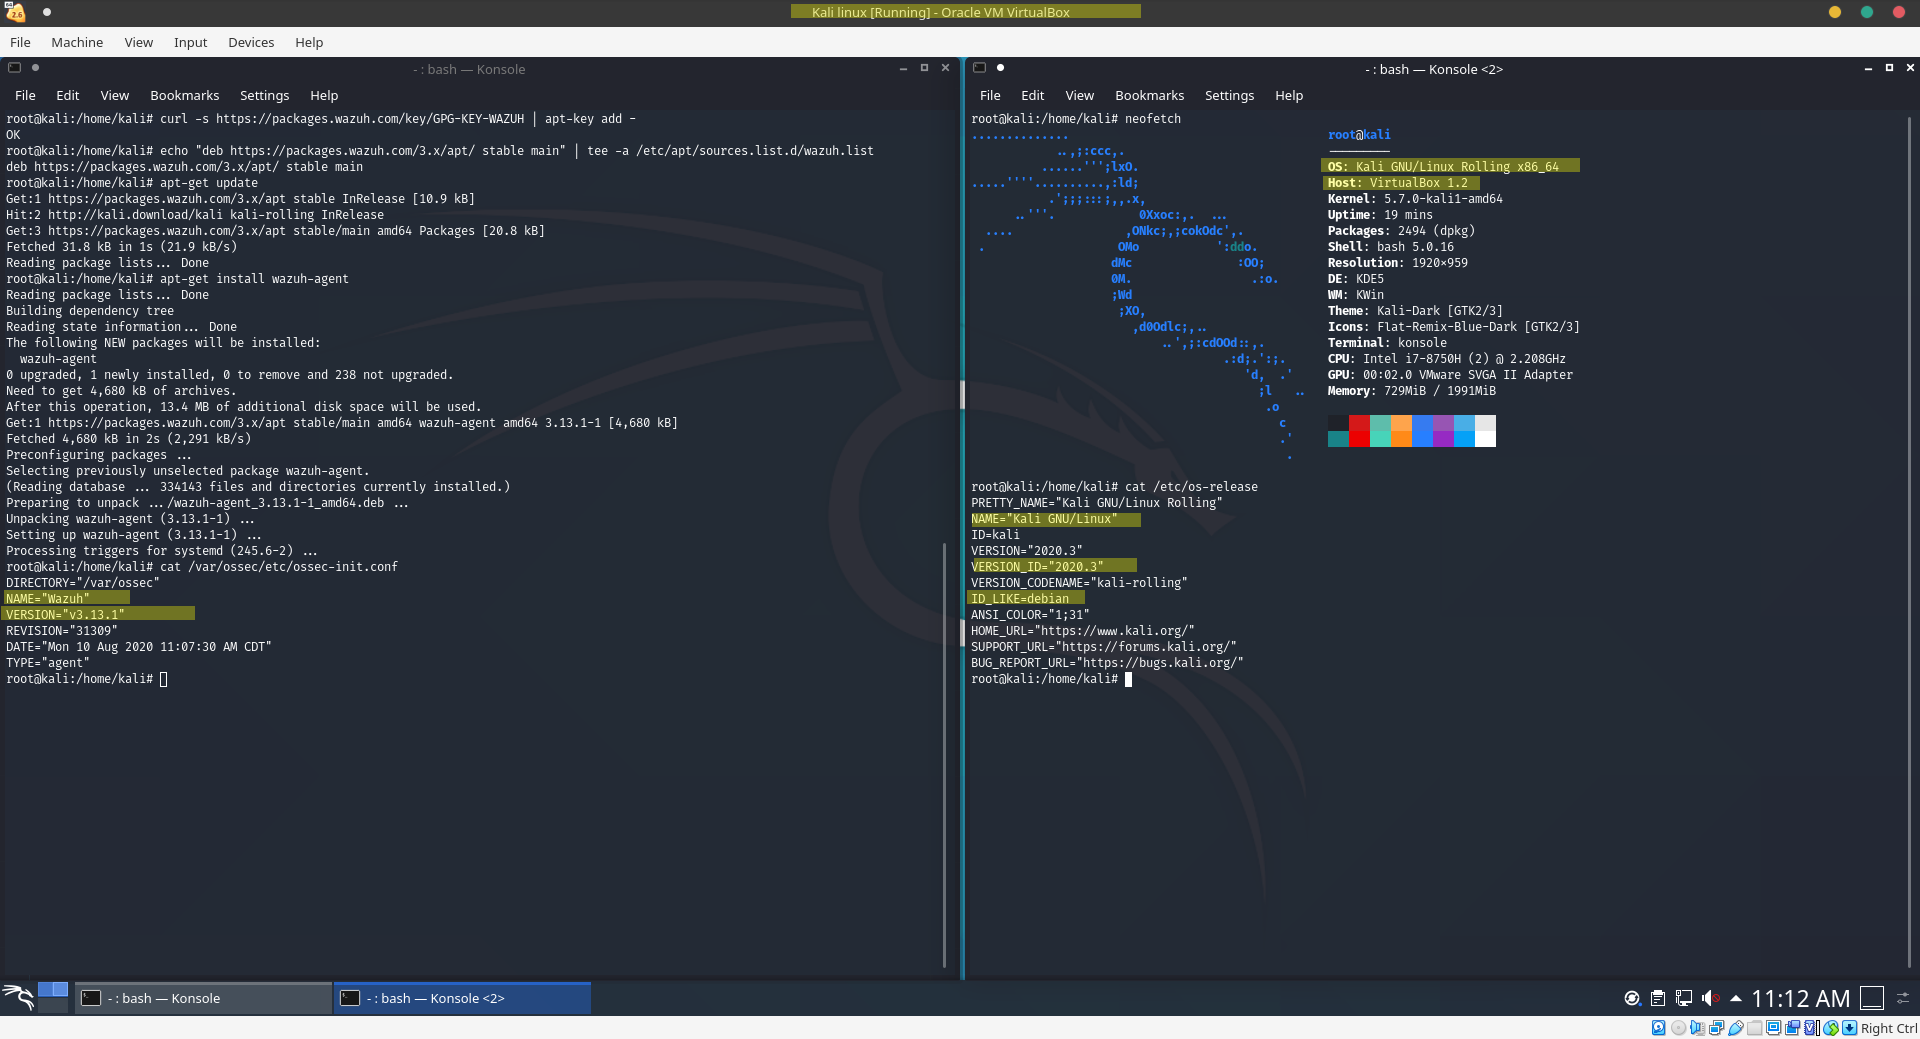
\includegraphics[width=\textwidth]{imagenes/kali_linux.png}
  \caption{Captura de pantalla del entorno virtualizado de Kali Linux mostrando alguna información del sistema y la instalación de Wazuh en varios terminales.}
  \label{kali1}
\end{figure}


Kali Linux es una \Gls{Rolling Release}, lo que significa que las actualizaciones se hacen de forma incremental y no tiene un versionado discreto. Para este estudio he utilizado una ISO etiquetada como \textbf{2020.04} (ver figura \ref{kali1} y la he instalado en una máquina virtual limpia. En el apartado siguiente discutiremos el uso de Wazuh en el proyecto y qué papel tendrá esta instancia desde la perspectiva de la arquitectura de Wazuh.

\subsection{Uso de Wazuh en Kali Linux}\label{sec:wazuh_kali}

Hemos hablado de varias formas de aprovechar Wazuh en una auditoría de seguridad. 

\begin{itemize}
    \item Por un lado, se podría \textbf{evaluar el rendimiento de la aplicación} ante un ataque simulado. Para ello, haría falta que el agente de Wazuh se encontrara instalado en la máquina que se va a evaluar y conectado a un Wazuh manager (preferiblemente instalado en otro dispositivo)  que además disponga de un servicio de Elasticsearch y Kibana.
    \item Por otro lado, queremos que Wazuh nos sirva para analizar y almacenar información extraída de los tests de penetración de sistemas. Para ello, necesitaríamos también dispone de un servidor de Wazuh manager de Wazuh (puede ser el mismo que para el caso anterior) junto con Elasticsearch y Kibana. Y necesitaremos otro agente de Wazuh instalado en la máquina `atacante' (Kali Linux) para recoger los datos generados durante la auditoría.
\end{itemize}

Una pregunta interesante sería si \textbf{verdaderamente hace falta un agente de Wazuh instalado en la máquina con Kali Linux}. La respuesta es que no es estrictamente necesario: existen otras formas de enviar datos a un Wazuh manager \textbf{sin hacer uso de un agente}, por ejemplo, utilizando un servicio \textbf{syslog} y enviando logs en ese formato al manager.

Esta opción sería perfectamente válida y eliminaría la necesidad de instalar y servir el agente de Wazuh, pero supondría otra necesidad: la de instalar y configurar un agente de syslog que sea capaz de enviar los logs a Wazuh. Además, una importante \textbf{ventaja de utilizar un agente Wazuh} es que sus mensajes se envían comprimidos y \textbf{encriptados} por defecto, lo que asegura una comunicación segura y es preferible a una comunicación con formato syslog (cuya seguridad depende del software utilizado y de su configuración y en algunas ocasiones no se tiene lo suficientemente en cuenta).

Por otro lado: hay que distinguir un caso de uso posible similar al que se describió en la introducción al hablar sobre \textbf{Faraday}, que es el de usar Wazuh como un entorno colaborativo de pentesting, en el que un equipo de profesionales del sector podría conectarse a \textbf{un mismo manager} de forma que, teniendo todos acceso a la aplicación web de Kibana, pudieran compartir sus logs e información extraída durante una auditoría.

Si no es el caso, y solo existe un único profesional que vaya a realizar la auditoría, y si además la empresa no cuenta ya con un entorno con Wazuh y Elasticsearch configurado, otra opción que se puede valorar es la de \textbf{instalar directamente el Wazuh manager en Kali Linux} junto con Elasticsearch y Kibana, puesto que el propio manager también es capaz de recopilar información del sistema dónde se encuentra (como si fuera un agente) y así eliminaríamos comunicaciones y la necesidad de tener más de un servidor funcionando. Un ejemplo de la diferencia entre estas dos maneras de utilizar Wazuh se muestra en la figura  \ref{entorno_ejemplos}.

\begin{figure}[!hbt]
  \centering
  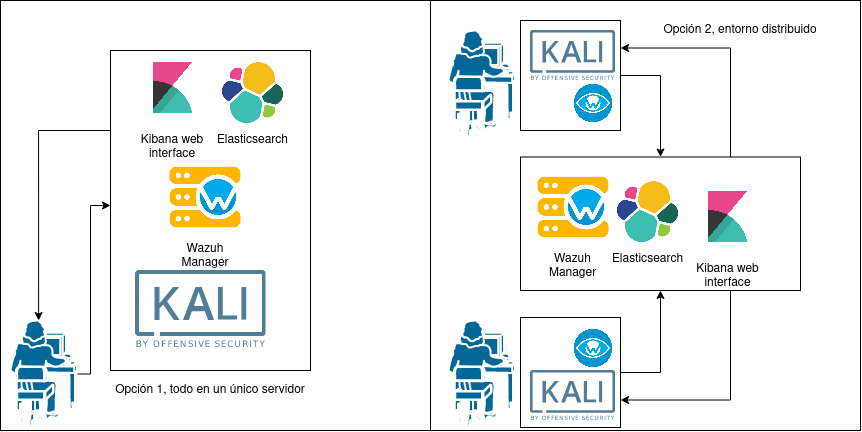
\includegraphics[width=\textwidth]{imagenes/entorno.png}
  \caption{Ejemplo de varias formas de distribuir los servicios para hacer uso de Wazuh. En la imagen de la izquierda se ve un entorno único, monousuario con todo instalado en una sola máquina y sin hacer uso de agentes, mientras que en la otra imagen se ve cómo podría distribuirse el entorno haciendo uso de agentes para ser utilizado por más de una persona.}
  \label{entorno_ejemplos}
\end{figure}


Para el trabajo se ha utilizado la opción de instalar un Mánager de Wazuh, así como el servicio de Elasticsearch y Kibana, todo en el mismo servidor con Kali Linux. Esto se ha llevado a cabo utilizando una máquina virtual, pero también podría realizarse por medio de Dockers, de forma que los distintos servicios se separaran por contenedores y se simplifica el despliegue de los mismos.

A este servidor se le conectará además un agente instalado en la máquina vulnerable que se estudiará en el caso práctico de la fase final.
\chapter{Análisis del problema de recopilación de datos de ejecución de comandos en consola\label{cap:Registro}}

En este capítulo se discutirán la técnicas para recopilar información durante una auditoría de seguridad. Se discutirá el problema de cómo almacenar la ejecución de comandos en un terminal, junto con sus meta-datos (tiempo de ejecución, usuario, directorio activo en el momento, etc...) y su output. 


\section{El problema del registro de ejecución de comandos en consola}

Como señala Damien King en su artículo "Logging Like A Lumberjack" \cite{logging}, existen múltiples motivos para registrar los comandos ejecutados durante cualquier procedimiento informático y en concreto, durante una auditoría de seguridad. A continuación se enumeran algunos de ellos.

\begin{description}
\item[Simplicidad] Evita realizar la misma prueba varias veces. En ciberseguridad, además, implica mayor discreción al evitar repetir la misma acción varias veces y además ahorra tiempo cuando esa acción que se evita repetir tiene una duración considerada.
\item[Reportes] Sirve como base o complemento para escribir un buen reporte, permite hacer estadísticas o investigaciones exhaustivas si se añaden meta-datos como la duración de la ejecución de cada comando, el usuario efectivo del mismo, momento de la ejecución, etc...
\item[Responsabilidad] En el caso de una auditoría de seguridad, tener un registro de los comandos ejecutados contra los servidores de un cliente (enriquecidos con información como la hora de ejecución) puede ser muy útil cuando hay algún problema para delimitar la responsabilidad de las acciones del auditor en el caso de que hubiera algún tipo de investigación.
\item[Contrato] Es posible que los clientes especifiquen en el propio contrato del trabajo que es necesario registrar los comandos y acciones llevadas a cabo contra el sistema.
\item[Reproducibilidad] Llevando un registro de nuestros tests podremos replicarlos o imitarlos en un futuro si fuera necesario. 
\item[Distribución] Permite compartir y distribuir los pasos seguidos durante una auditoría (u otro procedimiento) y facilita entender o hacer llegar los resultados y conclusiones.
\item[Automatización] Un problema relacionado con la automatización de tareas propias del hacking ético (o de cualquier ámbito informático) es la necesidad de notificar de aquellos eventos de interés que suceden durante el proceso automático. Ya sea de un error o porque el proceso ha conseguido llevar a cabo algo. Registrar la ejecución de los comandos ejecutados y sus salidas podría ser un punto de partida para distintas automatizaciones.
\end{description}
\label{razones_log}

Si bien existen multitud de formas de registrar los comandos ejecutados en una consola de comandos, la mayoría de estas opciones \textbf{están limitadas}. 

A continuación, valoraremos cuáles son los requisitos que se podría esperar de una buena solución para el registro de ejecución de comandos, se describirán algunas opciones y se propondrá una respuesta al problema de la captura de comandos en un terminal.

\subsection{Características deseables de una solución}

\begin{description}
    \item [Registro de comando y output] Debe permitir almacenar la salida de la ejecución de un comando junto con el comando en sí, puesto que la salida puede contener información relevante para el estudio.
    \item [Metadatos] Debe permitir obtener todos los meta-datos posibles sobre la ejecución de cada comando: usuario efectivo, hora y fecha de la ejecución, directorio activo en el momento de la ejecución, hostname del servidor donde se ha ejecutado, si se ejecutó o no con permisos de administración, etc...
    \item [Extensible a sesiones externas] Debe ser extensible a sesiones externas (ssh) para que sea posible registrar las partes de una auditoría que tienen lugar en aquellos hosts a los que se consigue acceso (escalado de privilegios, eliminación de pruebas, etc...), a ser posible debe poder usarse sin disponer de permisos de administrador.
    \item [Lógica sencilla] Preferiblemente, no debe requerir de una lógica completa que contemple muchas alternativas y posibles casos concretos (debe reaccionar bien ante cualquier comando que se ejecute y su output sin requerir para ello una lógica muy compleja y específica para cada caso).
\end{description}

\section{Soluciones al problema de captura de comandos}

A continuación, se enumeran algunas soluciones propuestas para el problema de la recopilación de datos (y metadatos) durante una sesión de consola de comandos. Se proponen algunas soluciones y se describen sus ventajas e inconvenientes.

\subsection{Comando script}

\textit{Script} es un comando de Linux/Unix que permite almacenar en un fichero todo lo que se escribe en una consola de comandos, es decir: tanto los comandos ejecutados por el usuario como la salida de los mismos.

El fichero generado puede ser enviado a Wazuh pero su formato está destinado a humanos más que a computadores y \textbf{no es fácilmente decodificable}.

Además, si se quiere analizar la ejecución de comandos en todos los terminales que se ejecuten en el sistema, habríamos de iniciar la ejecución de \textit{script} en el inicio de cada sesión y esto puede causar problemas ya que cuando se ejecuta este comando se crea otra sesión (interna al comando) que lee los archivos de configuración y de inicio de sesión. Esto se traduce en un bucle infinito si tratamos de ejecutar \textit{script} al inicio de cada sesión interactiva.

Una solución sería añadir al(\textit{profile} (/etc/profile) del sistema el script \ref{session}

\begin{lstlisting}[language=bash,caption={Session recorder (/etc/profile)}, label=session]
if [ "x$SESSION_RECORD" = "x" ]
the
timestamp=$(date +%d-%m-%Y-%T)n
session_log=/var/log/session/session.$USER.$$.$timestamp
SESSION_RECORD=started
export SESSION_RECORD
script -t -f -q 2>${session_log}.timing $session_log
exit
fi
\end{lstlisting}

Esta solución, presenta la ventaja de que almacena todo lo que aparezca en la pantalla, incluyendo sesiones ssh, otras consolas (Python, zsh, bash, fish, mfsconsole...), etc.. sin embargo, presenta también los siguientes inconvenientes:

\begin{itemize}
    \item El formato del resultado no es decodificable de forma trivial, existen multitud de casos en los que cuesta distinguir dónde acaba un comando y empieza el siguiente.
    \item El resultado incluye caracteres especiales de formato (colores, negrita, etc...) propios de las consolas de comandos que, si bien se podrían eliminar, hacen que la solución sea aún más aparatosa.
    \item Saltos de línea, espacios y demás aparecen en el fichero final. Si se ejecutara, por ejemplo, el comando \textit{clear}, se almacenaría en el resultado tantos saltos de línea como imprimiera dicho comando.
\end{itemize}

Cabe mencionar que se ha estudiado la posibilidad de utilizar \textit{script} junto con otra herramienta que analizara en tiempo real la salida de script y filtrara los caracteres especiales, además de tratar de separar los comandos entre sí y con su ejecución y escribirlos en un formato que pudiera ser decodificado por Wazuh.

No obstante, tras trabajar en dicha opción se llegó a la conclusión de que era demasiado aparatoso separar los comandos entre sí y de sus salidas y darles un formato fácil de analizar por Wazuh u otras herramientas.

Aún así, se trata de una opción perfectamente válida para registrar sesiones y podría ser utilizada como base para la creación de un módulo de logging para Wazuh.

\subsection{Trampas de Linux}

Una posible alternativa al comando script es utilizar las "trampas" (traps) de Linux, utilizando el comando \textbf{trap} se puede definir otro comando que se ejecutará antes de cualquier comando introducido en una shell. Así, se podría registrar la salida de cada comando (así como el comando introducido en sí) y calcular información como el nombre del usuario que lo ejecutó  o el momento de ejecución del comando (recopilación de metadatos). Ver \ref{trampas}

\begin{lstlisting}[language=bash,caption={Session recorder (on bashrc file) \newline Fuente: https://unix.stackexchange.com/questions/250713/modify-all-bash-commands-through-a-program-before-executing-them}, label=trampas]
shopt -s extdebug

preexec_invoke_exec () {
    [ -n "$COMP_LINE" ] && return  # do nothing if completing
    [ "$BASH_COMMAND" = "$PROMPT_COMMAND" ] && return # don't cause a preexec for $PROMPT_COMMAND
    local this_command=`HISTTIMEFORMAT= history 1 | sed -e "s/^[ ]*[0-9]*[ ]*//"`;

    # So that you don't get locked accidentally
    if [ "shopt -u extdebug" == "$this_command" ]; then
        return 0
    fi

    if [[ "${this_command}" =~ \S*=.* ]]; then
      this_command_output=""
      echo "$(date '+%Y-%m-%d %H:%M:%S') $(whoami)@$(pwd)# ${this_command}: $this_command_output"
      return 0
    fi

    this_command_output=$(eval "${this_command}" | tee /dev/tty)
    this_command_output=$(echo "${this_command_output}" | tr '\n' ' ')

    echo "$(date '+%Y-%m-%d %H:%M:%S') $(whoami)@$(pwd)# ${this_command}: $this_command_output"
    # Modify $this_command and then execute it
    return 1 # This prevent executing of original command
}
trap 'preexec_invoke_exec' DEBUG
\end{lstlisting}

Esta solución permite analizar los comandos ejecutados en el sistema y su output pero presenta algunos inconvenientes que llevan también a descartarlo:

\begin{itemize}
    \item Problemas con comandos que modifican la forma en que se redirija el output a la pantalla (editores de texto como VIM o emacs, por ejemplo).
    \item A priori no permite definir variables en el shell, salvo que se atrape aquellos comandos que sirvan para definirlas de forma especifica y se permita su correcta ejecución, lo cual podría ser problemático en algunas circunstancias que habrían de estudiarse.
    \item Hay que evitar la ejecución del comando `clear' porque escribiría nuevas líneas en el output al igual que ocurría con el comando \textit{script}.
    \item Hay que gestionar de forma diferente comandos como `cd' y otras utilidades de Linux, puesto que si se capturan, el resultado esperado (como moverse a otro directorio) no se daría.
    \item No puede monitorizar nada que se ejecute en remoto (ssh) o en otro tipo de consolas salvo que se ejecute el comando al inicio de la sesión y solo funcionaría en consolas compatibles con bash.
\end{itemize}

\subsection{Kernel modules, ptrace, system calls}

Una posible opción (sencilla pero que requiere conocimientos de OS a bajo nivel) podría ser añadir un módulo de kernel que modifique las llamadas al sistema utilizando \textit{ptrace} y que obligue a todos los procesos del sistema operativo a duplicar su STDOUT al descriptor del proceso y a un fichero (de forma que toda la STDOUT quede registrada) al inicio del mismo, y en la llamada a \textit{exit} cree un mensaje que se escribiría en algún fichero con el comando ejecutado, sus argumentos y su salida. 

Sin embargo esta opción tampoco nos permitiría registrar comandos ejecutados en otros sistemas, por ejemplo usando SSH o SFTP y sería muy poco portable. 

\subsection{Auditd}

Audit es una herramienta que, permite monitorizar las llamadas a funciones del kernel para, entre otros, detectar cambios en ficheros o ejecución de comandos. Es una opción muy útil y, de hecho, Wazuh la utiliza para registrar ejecución de comandos en los servidores dónde se encuentra instalado, pero \textbf{no permite capturar la salida de los comandos} y además es muy poco portable puesto que requiere de permisos de administración para utilizarse.

\subsection{Usando descriptores de procesos: TTY, STOUT, STDERR}

El siguiente paso ha sido tratar de entender cómo funciona el emulador de terminal en que se ejecutan los comandos, su TTY y los ficheros del proceso que determinan la entrada y salida estándar (STDIN, STDOUT) así como la salida estándar de error (STDERR) y tratar de utilizarlas de forma que se pudieran procesar en tiempo real para adecuarlas al input que Wazuh podría esperar de nuestros registros.

Se ha dedicado un tiempo considerable a esta opción y, no obstante, han aparecido muchos problemas derivados de la complejidad de trabajar con los ficheros de los procesos. Las razones para descartarla han sido:

\begin{itemize}
    \item No es una solución portable puesto que requiere trabajar con los descriptores de fichero de los procesos del sistema, lo cual necesita permisos de administrador.
    \item Aunque existe la posibilidad de capturar la entrada y salida de comandos como SSH o mfsconsole, el capturar dichos comandos interfiere en la forma en que esas herramientas funcionan y \textbf{puede empeorar la experiencia de usuario}
\end{itemize}

\subsection{Una consola de comandos específica que permita capturar los datos de forma más específica}

Otra solución sería una consola propia, de forma parecida a lo que hace \textbf{Faraday}, de forma que podamos ejecutar una shell pero además incluir funcionalidad extra como la recopilación de metadatos y el formateo de la información como se prefiera.

El desarrollo de la misma se discutirá en una sección posterior.

\subsection{Comparativa de las soluciones propuestas}

\begin{table}[]
\resizebox{\textwidth}{!}{
\begin{tabular}{|l|l|l|l|l|}
\hline
Solución                  & Almacenar entrada y salida correctamente    & Metadatos & Portable & Lógica sencilla \\ \hline
Script                    & No, problemas de formato                    & No        & Sí       & Sí              \\ \hline
Script con análiSís extra & No, no se pueden contemplar todos los casos & Sí        & Sí       & No              \\ \hline
Trampas Linux             & Sí                                          & Sí        & No       & No              \\ \hline
Módulos del kernel        & Sí                                          & No        & No       & No              \\ \hline
Auditd                    & No                                          & Sí        & No       & Sí              \\ \hline
Descriptores de procesos  & Sí                                          & Sí        & No       & No              \\ \hline
Consola/shell específica  & Sí                                          & Sí        & Sí       & No              \\ \hline
\end{tabular}
}
\caption{Tabla comparativa de las soluciones propuestas}
\label{soluciones_comparativa}
\end{table}

En la tabla \ref{soluciones_comparativa} se comparan las soluciones propuestas en base a las características deseables que describimos inicialmente.

Respecto a la creación de un shell específico: dado que podríamos controla la ejecución de los comandos y su output y acompañar esto de una lógica interna de la shell nos permitiría añadir metadatos. Sobre la portabilidad de la misma: habría que buscar la manera de capturar correctamente los comandos ejecutados en sesiones de SSH o de otro tipo de consola pero se podría diseñar de forma que no hiciera falta instalar ningún programa para utilizarlo. En la sección final se describe la solución final adoptada y cómo se afronta esta problemática.


\section{Análisis del enfoque: Consola de comandos propia para tests de penetración de sistemas}

Para crear una consola de comandos propia a Wazuh que permitiera resolver la problemática descrita se barajan múltiples opciones. Se ha invertido algo de tiempo en cada una de ellas para a continuación describir las ventajas e inconvenientes de cada una y, finalmente, tomar una decisión final.


\subsection{Creación de un nuevo proyecto}

Al igual que en el proyecto Faraday, otra opción válida podría ser crear un emulador de consola de comandos o una shell nueva para el proyecto, en lugar de modificar una existente.

Al contrario de lo que cabría esperar, no hay muchos proyectos de calidad en lo que a emuladores de terminales se refiere, además de los más conocidos (Gnome shell, Konsole, terminator...) y algunos proyectos menores escritos en otros lenguajes como Python, ruby o go, pero los hay o demasiado complejos (y escritos en lenguajes como C) o demasiado simples y con poco soporte de la comunidad (proyectos deprecados, con poca participación en Github o con muy poca actividad). 

Por otro lado, se han analizado dos proyectos interesantes que podrían permitir escribir un emulador de terminal con mayor facilidad.

\begin{itemize}
    \item Ruby TTY toolikt\footnote{\url{https://github.com/piotrmurach/tty#4-contributin}}
    \item Python prompt toolkit\footnote{\url{https://github.com/prompt-toolkit/Python-prompt-toolkit}}
\end{itemize}

El primer proyecto, en Ruby, tiene una buena documentación y un buen diseño, aunque es bastante menos activo que el segundo y está hecho en un lenguaje, en general, poco conocido. 

Se ha valorado utilizar \textbf{Python prompt toolkit} porque es un proyecto más activo, escrito en un lenguaje más popular (y más afín al proyecto de Wazuh).

Sin embargo, tras muchas horas de dedicación al proyecto se puede concluir que la dificultad de crear una consola desde cero es demasiado grande para que el proyecto pudiera ser interesante a la comunidad. Tras consultarlo con el tutor, se concluyó que llevar esto a cabo requeriría una planificación exhaustiva, mayores recursos y tiempo del que corresponde a un trabajo fin de grado. 



\subsection{Modificación de proyectos existentes}

La segunda opción valorada es modificar un proyecto existente. Ya se comento en el apartado referido al estado del arte \cite{sec:estado del arte} que existen muchas opciones en las distintas herramientas relacionadas con consolas de comandos para generar un historial de comandos, pero la mayoría no contempla \textbf{la necesidad de almacenar la salida y otros metadatos de los mismos}. Al igual que mencionamos que el proyecto \textit{Fraday} \textbf{tiene su propia terminal} con algunas características especiales que permiten alterar la ejecución de los comandos para hacerlos más fáciles de analizar, en este trabajo se plantea si se podría afrontar este problema utilizando un proyecto existente de `emulador de terminal' y modificarlo (o añadirle alguna extensión) para la recopilación de los datos.

En este caso, se han trabajado varias opciones: 

\begin{itemize}
    \item \textbf{Alacritty} \footnote{\url{https://github.com/alacritty/alacritty}}, un proyecto opensource de emulación de terminal escrito en Rust, un lenguaje recientemente creado por Mozilla que resulta bastante rápido y funcional. Sin embargo, el desconocimiento del lenguaje y la complejidad del proyecto, además de la poca ayuda encontrada por parte de la comunidad del mismo me ha llevado a descartarlo como opción.
    \item \textbf{Terminator} \footnote{\url{https://github.com/gnome-terminator/terminator}}, un proyecto opensource de emulación de terminal escrito en Python y basado en \textbf{gnome-shell}. Esta opción ha dado muy buenos resultados y se discute a continuación.
\end{itemize}


Se preparó una prueba de concepto basada en un \textbf{plugin para terminator}\footnote{\url{https://github.com/gnome-terminator/terminator/blob/master/terminatorlib/plugins/logger.py}} que permite registrar información de los comandos ejecutados en el emulador. A partir de este se ha conseguido:

\begin{itemize}
    \item Separar correctamente la ejecución de comandos entre sí, con la entrada y salida bien diferenciadas. Almacenando el resultado en un formato adecuado para ser decodificado
    \item Obtener metadatos de los comandos ejecutados.
    \item Una implementación con una lógica sencilla.
\end{itemize}

Dicho plugin está \textbf{disponible en Github}\footnote{\url{https://github.com/spothound/auditor.py}}

Esta opción es interesante y ha servido como base para empezar a integrar los comandos ejecutados con Wazuh, no obstante presenta el inconveniente de \textbf{requerir el uso de terminator} de forma obligatoria (lo que condiciona la experiencia de usuario), junto con la aparición de numerosos problemas al tratar de capturar los comandos ejecutados en una sesión SSH (en otro host), es una buena solución, pero mientras trabajábamos en ella encontramos otra alternativa que nos resultó más interesante.


\subsection{Análisis del proyecto Xonsh}

Como parte de la investigación sobre herramientas de emulación de shell, multiplexores, \textit{shells}, etc... se ha analizado un proyecto llamado \textbf{Xonsh}\footnote{https://xon.sh/}. Una consola interactiva de comandos \textbf{escrita en Python} con una fuerte base de soporte para \textit{plugins} que es compatible con la sintaxis de otras shells más comunes (como bash y zsh) además de \textbf{tener la sintaxis de Python}.

Utilizando plugins de Xonsh podemos añadir cualquier lógica a la ejecución de comandos, lo que nos permite fácilmente obtener metadatos sobre los comandos ejecutados y, dado que el propio shell tiene una lógica que analiza el input del usuario para ejecutar de una forma u otra los comandos, es bastante sencillo separar el input del output y \textbf{gestionar la ejecución de comandos problemáticos como \textit{clear} o \textit{vim}}. 

Por si fuera poco, existe un proyecto \textbf{creado a partir de Xonsh}, \textbf{XXH}\footnote{\url{https://github.com/xxh/xxh}}, diseñado para actuar como una capa de abstracción para comunicaciones a través de SSH que permite envíar en el momento de conexión con otro servidor una imagen portable de Xonsh a la máquina remota con las configuraciones y plugins presentes en el host local. 

Se puede, por tanto, crear una herramienta que haga uso de Xonsh y XXH y de un par de plugins extra para ambos de forma que:

\begin{itemize}
    \item Se registren los comandos ejecutados en Xonsh en la máquina local
    \item Cuando se establezca una conexión ssh con un host remoto se le envíe una imagen portable de la consola con el plugin necesario para guardar los registros
    \item Durante la sesión o al finalizar esta, se recuperen los logs generados en remoto (y enriquecidos gracias a Xonsh) y se almacenen en local
    \item Al final de la sesión se borren todos los archivos generados por XXH, que, por defecto, descarga los archivos necesarios para ejecutar Xonsh en un directorio aislado y oculto dentro del directorio \textit{home} del usuario.
\end{itemize}

Si bien esta solución también `obliga' al usuario a usar, no ya un emulador de terminal concreto (en este caso el usuario podría usar el que prefiera) sino un shell concreto (aunque Xonsh es compatible con la sintaxis de bash y de zsh, tiene algunas cosas que son diferentes), es una opción \textbf{muy versátil} que nos permitiría llegar a crear una shell específica para pentesting. Es muy fácil crear plugins, trabajar con los comandos y sus metadatos, etc.. y la integración con XXH hace que sea una opción \textbf{muy especial} puesto que el \textbf{reto de registrar los comandos ejecutados en un host remoto a través de ssh} no se puede solucionar fácilmente con la mayoría de las opciones propuestas y con esta sí.




\chapter{Diseño y desarrollo de un framework para hacking ético integrable con Wazuh: OffSh} 

\section{Introducción}

Xonsh es una shell que admite la sintaxis en Python pero que, además, puede ejecutar comandos con sintaxis propia de bash o zsh. Tiene un backend para crear un historial \textbf{dinámico y enriquecido} que servirá para extraer los metadatos interesantes de la ejecución de comandos y, adicionalmente, su funcionamiento \textbf{puede ser modificado y extendido con plugins utilizando un soporte nativo para éstos}. 

Para solucionar el problema del registro de ejecución de comandos se puede crear una extensión que permita modificar el backend del historial de comandos, para enriquecer la información almacenada y redirigirla del modo que queramos (a un fichero JSON, syslog, o enviarla directamente a Wazuh son algunas de las opciones) \cite{prompttoolkit}\cite{Xonshdocs}.

\subsection{Desarrollo y control de versiones}

Para albergar el código de este proyecto se ha creado una organización en Github llamada \textbf{Offsh}\footnote{\url{https://github.com/offsh}}(Offensive Shell) y en ella he creado un plugin para Xonsh llamado \textbf{xontrib-syslog-profiler}\footnote{\url{https://github.com/offsh/offsh}, en Xonsh, a los plugins se les llama xotribs, de ahí el nombre.}. 

Se ha utilizado Github por ser un portal de git (controlador de versiones) muy conocido que ademas tiene un sistema de `acciones' que permite automatizar tareas de despliegue y que se ha utilizado para \textbf{desplegar el plugin en la plataforma de Pypi de forma que pueda ser instalado usando el comando ``pip'}. Este despliegue se hace automáticamente usando un `github action' cada vez que se crea un Tag (release) de una nueva versión del plugin (ver Figura \ref{githubactions}).

\begin{figure}
  \centering
  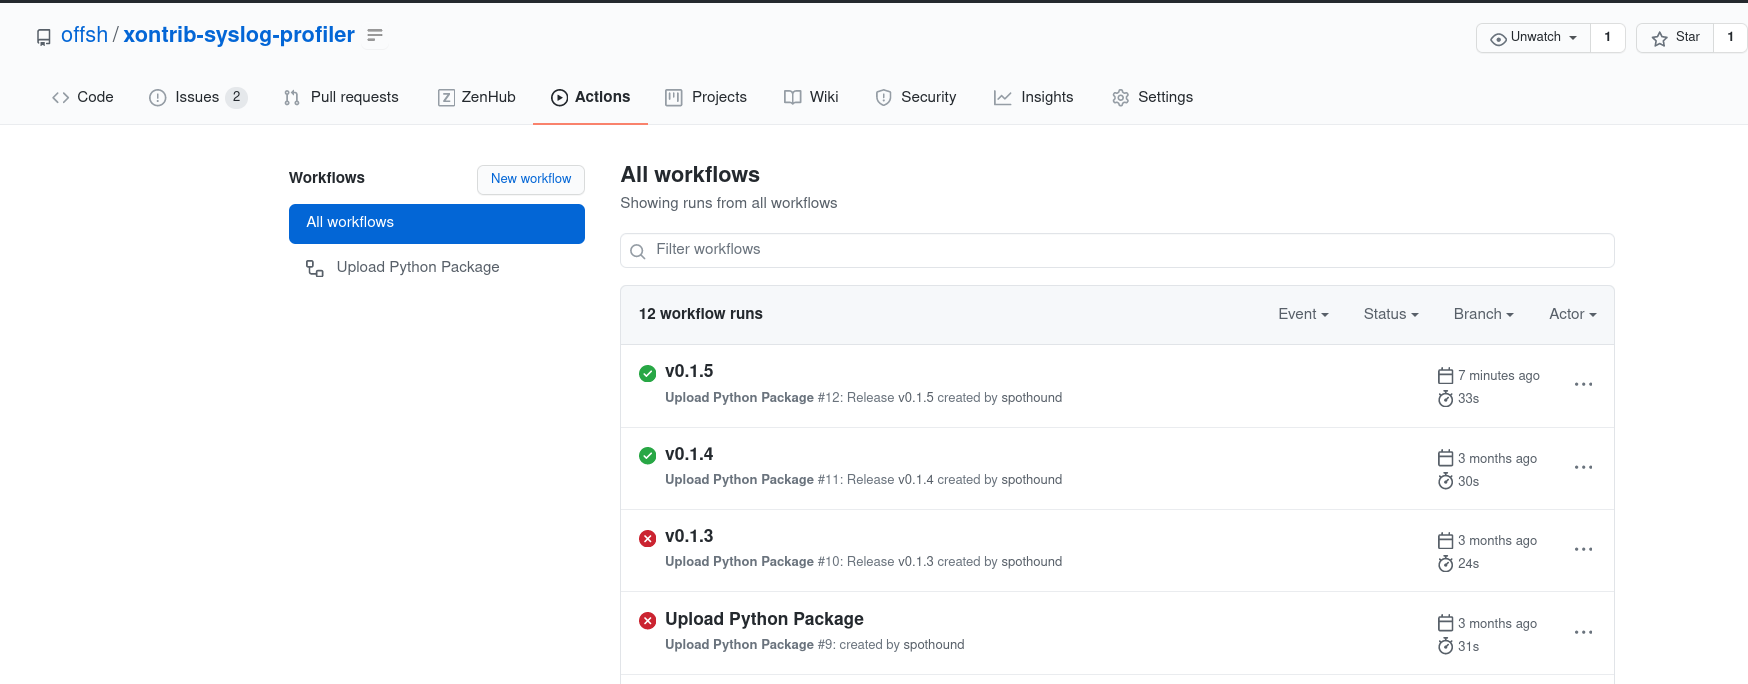
\includegraphics[width=\textwidth]{imagenes/githubactions.png}
  \caption{Ejemplo del uso de Github actions para el despliegue del plugin en Pypi. En ella se aprecia cómo, de forma automática, Github lanza una serie de scripts cuando se genera un nuevo `tag' del código y sube el nuevo paquete al repositorio de pip.}
  \label{githubactions}
\end{figure}

Este plugin hace que todos los comandos ejecutados en Xonsh se guarden en un registro (común a todas las terminales). Basta con instalar el plugin y activarlo en el archivo de configuración de Xonsh para empezar a generar los registros en un fichero predeterminado.

Además, el proyecto incluye un archivo especial de configuración con algunas opciones interesantes para darle un aspecto visual diferente al shell original. Entre estas mejoras, se ha añadido un prompt en forma de barra, que asigna un color aleatorio (dentro de un rango, acorde con el fondo) al nombre de usuario, dominio y directorio activo. De esta forma, cuando se pasa de un host a otro utilizando xxh, se puede apreciar fácilmente el cambio de host y/o de usuario (ver Figura \ref{offsh_example}).


\begin{figure}[!hbt]
  \centering
  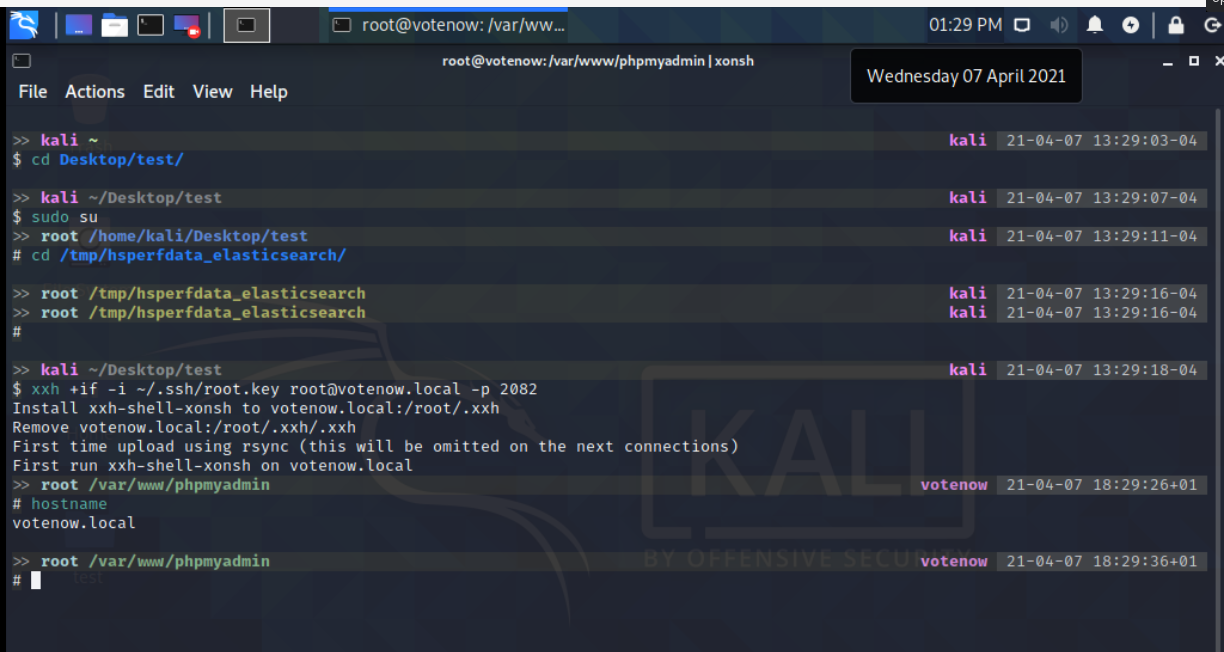
\includegraphics[width=\textwidth]{imagenes/offsh_Example.png}
  \caption{Visualización del uso de offsh con un cambio de host usando xxh. En la imagen se aprecia como el prompt (en barra) muestra el usuario activo, el hostname, directorio actual y el momento de ejecución de cada comando. Esta información (excepto el tiempo) tiene un color determinado por un hash del nombre (de usuario, hostname o path) de forma que el color cambia cuando alguno de estos aspectos cambia también.}
  \label{offsh_example}
\end{figure}


\subsection{Otros usos para el framework}

El framework desarrollado permite montar imágenes modificadas de Xonsh con las características y plugins que se quieran. Como además el plugin que registra los logs que se ha diseñado utiliza el formato syslog, esta funcionalidad podría integrarse con \textbf{cualquier otro software además de Wazuh}. Y los shells creados podrán usarse para distintas funcionalidades.

\begin{figure}[!hbt]
  \centering
  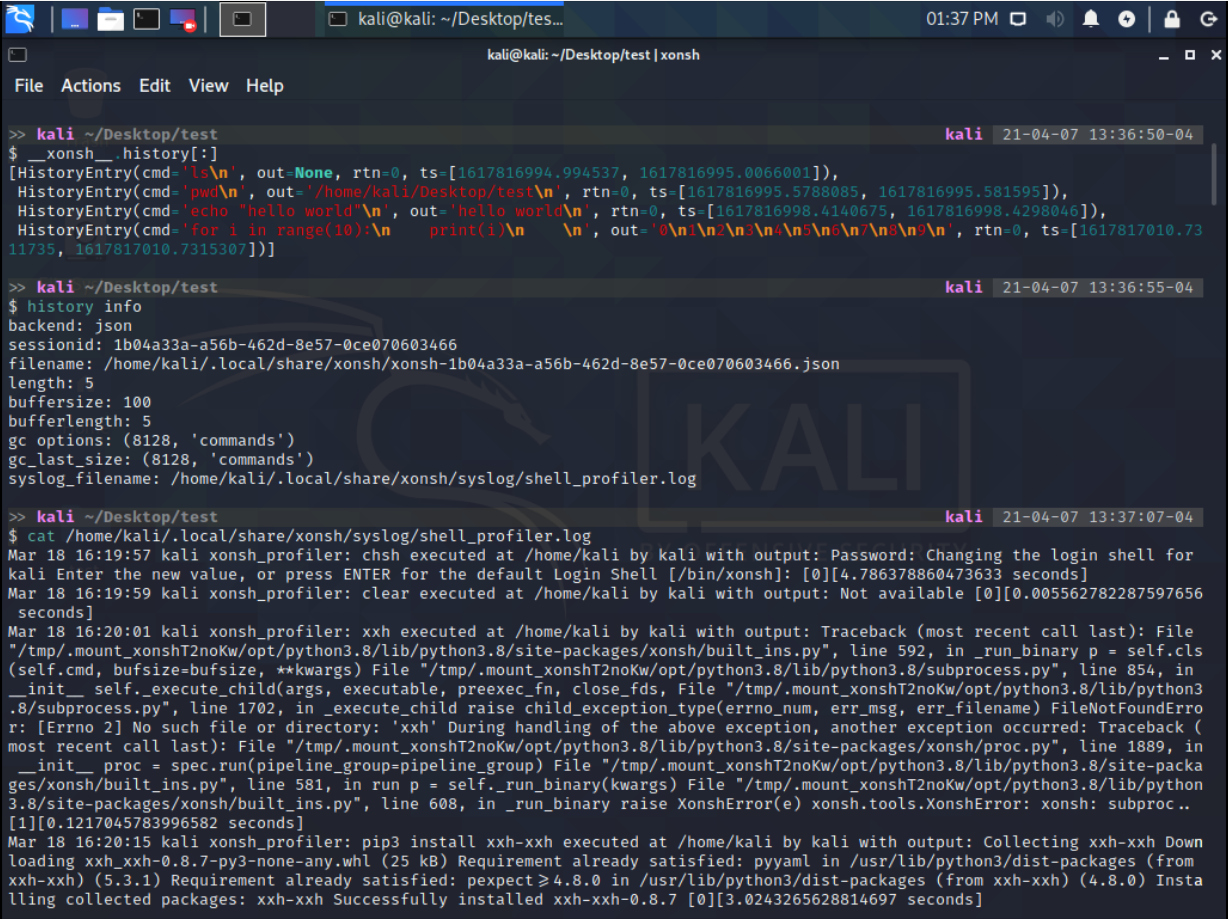
\includegraphics[width=\textwidth]{imagenes/syslog_plugin.png}
  \caption{Ejemplo del fichero generado por el plugin, así como de la forma que tiene Xonsh de almacenar la información (como un objeto Python). En el primer comando ejecutado se ve un mapa con los comandos y sus metadatos, a continuación se usa `history info' para obtener información del backend del historial de Xonsh y se hace un cat del archivo de syslog generado, que contiene la información con el formato que genera el plugin de syslog.}
  \label{syslog_plugin}
\end{figure}

En el apendice \ref{ISE} se expone un ejemplo del uso del mismo, con una propuesta de texto que podría ser incluido en las prácticas de la asignatura de Ingeniería de Servidores (ISE) del Grado en Ingeniería Informática de la Universidad de Granada, con o sin modificaciones. Así como un ejemplo en la Figura \ref{syslog_plugin} de los logs generados.





\subsection{Envío de los logs a Wazuh}

Sobre el envío de los registros a Wazuh, ya se ha discutido en el capítulo anterior (sección \ref{sec:wazuh_kali}) cuales serían las alternativas posibles. Básicamente se trata de enviar el fichero generado por Xonsh al manager, bien usando el agente de Wazuh o un cliente de syslog. Para el caso de uso práctico del capítulo final, por simplicidad, utilizaremos la otra opción propuesta: instalar \textbf{directamente el Wazuh Manager} en el entorno con Xonsh y configurarlo para que lea directamente el archivo con los registros.

La configuración necesaria está brevemente explicada en el repositorio de Github y es la que aparece en el Listado \ref{wazuh_conf}.

\begin{lstlisting}[language=bash,caption={Configuración necesaria para que Wazuh analice los logs generados por Xonsh}, label=wazuh_conf]
<localfile>
  <location>/home/*/.local/share/Xonsh/syslog/shell_profiler.log</location>
  <log_format>syslog</log_format>
</localfile>
\end{lstlisting}



\section{Análisis de los registros y generación de alertas}

Para que Wazuh pueda analizar los registros generados e indexarlos necesitamos algunas reglas y decodificadores adicionales en el conjunto de reglas ($ruleset$) de Wazuh.

Se utilizará un único decoder base (puesto que hemos configurado el plugin de Xonsh para escribir en el registro todos los registros con el mismo formato) que extraiga la información relevante de los comandos  una regla sencilla para generar alertas con la ejecución de comandos. A continuación, se desarrollarían alertas más concretas para determinados comandos o salidas de los mismos e incluso se podrían hacer decodificadores ({\it decoders}) especiales para \textbf{extraer información adicional de la ejecución del comando} como por ejemplo opciones utilizadas o algún elemento interesante de la salida del mismo.

Un detalle importante a tener en cuenta es que el sistema de análisis de registros de Wazuh funciona con una lógica estructurada en árboles de decisión para generar las alertas. Una vez un registro es decodificado por un decoder, se comprueba si concuerda con alguna de las reglas del primer nivel y, si lo hace, entonces se evalúan reglas hijas de la regla que ha coincidido con el registro. Se repite el proceso hasta que no hay más reglas hijas que concuerden con el log y entonces se \textbf{genera una única alerta} a partir de esta última regla. Ver Figura \ref{wazuhtree} para un ejemplo ilustrado.

Teniendo esto en cuenta, podemos crear distintas alertas cada vez más específicas y con distintos grupos y niveles según lo importante que pueda ser la ejecución de ese comando y el tipo de acción que se lleva a cabo. Por ejemplo, algunos grupos en los que agrupar alertas podrían ser:

\begin{itemize}
    \item reconocimiento
    \item ocultación
    \item vulnerabilidades
    \item escalada de privilegios
\end{itemize}

Y según la importancia de cada evento se le asignaría un nivel u otro a la alerta.


\begin{figure}[!hbt]
  \centering
  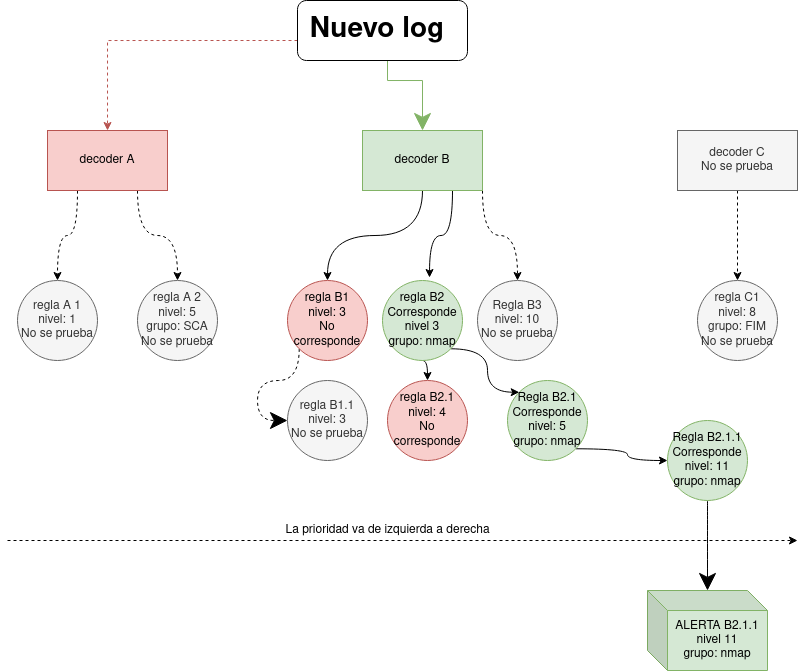
\includegraphics[width=\textwidth]{imagenes/arbol_wazuh.png}
  \caption{Ejemplo gráfico de cómo funciona la lógica de alertas y decoders de Wazuh. Cada decoder tiene una o varias reglas asociadas y estas pueden o no tener hijas. Se van leyendo los decoders hasta que uno coincide con el log de entrada, entonces se van leyendo las reglas en orden hasta que una coincide y esto se repite con las hijas de esta regla hasta que una ya no tiene más hijas (que coincidan con el log), entonces se genera una alerta basada en esa regla.}
  \label{wazuhtree}
\end{figure}




\section{Trabajar con logs de dispositivos externos utilizando XXH}

Ya hemos hablado de XXH, un proyecto complementario a Xonsh que nos permite utilizar una imagen portable de Xonsh (con un \textbf{Python embebido} que nos permite ejecutarlo sin necesidad de tener Python en el sistema) en hosts remotos a los que conectemos por SSH. 


Una primera decisión a tener en cuenta sería \textbf{cómo y cuando obtener los logs de las sesiones externas}, es decir, aunque se use XXH para ejecutar una versión portable de Xonsh que registre la información de los comandos en un fichero remoto (en la máquina accedida), se necesita un mecanismo para enviar dichos logs de nuevo al dispositivo desde el que se abrió la conexión.

La opción más transparente al usuario es modificar XXH para que utilice los mismos credenciales y protocolos que utiliza para \textbf{enviar la imagen portable de Xonsh} y descargue los registros generados en el dispositivo remoto.

Para ello se ha diseñado una versión de XXH\footnote{\url{https://github.com/offsh/xxh}} (a partir de un \gls{fork}) con las modificaciones necesarias para poder ejecutar `plugins' que permitan reutilizar los credenciales de conexión para establecer segundas conexiones de ssh o tcp/rsync, que se usarían para obtener los logs. Además, he creado un plugin\footnote{\url{https://github.com/offsh/xxh-plugin-local-syslog-profiler}} que permite descargar los registros generados en el dispositivo remoto. 



Además, se ha diseñado un pequeño archivo de configuración\footnote{\url{https://github.com/offsh/offsh/blob/main/Xonshrc}} para Xonsh, con algunas modificaciones para mejorar la experiencia de usuario (un prompt visualmente atractivo, colores diferentes según el host en el que estemos trabajando y el nombre de usuario, etc..), plugins de Xonsh que pueden resultar útiles durante las auditorías, alias y demás.

Otra opción que también se ha barajado sería crear un plugin o una funcionalidad para Xxh de `directorios compartidos'. Al igual que hacen algunos software de virtualización (como Virtualbox o Docker), aprovechando la potencia de XXH se podría plantear dicho módulo y utilizarlo para \textbf{sincronizar en tiempo real los resultados de las sesiones remotas}. Esta funcionalidad no se ha implementado como parte del proyecto pero se valora como una posible alternativa de mejora para la opción (más simple) escogida.

De cualquier modo, XXH es una herramienta que se ha incluido de forma nativa (el fork creado a partir de la rama principal de desarrollo) en el framework puesto que consideramos que las funcionalidades que aportan son muy importantes para el desarrollo de distintas consolas de comandos que puedan construirse con las herramientas diseñadas.

Para más información, ver figuras \ref{infographic} y \ref{diagramica}

\begin{figure}[!hbt]
  \centering
  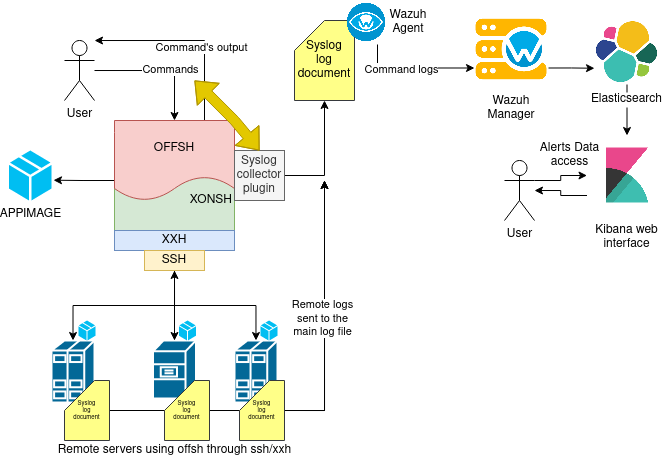
\includegraphics[width=\textwidth]{imagenes/diagramaflujo.png}
  \caption{Diagrama de flujo de datos e información en el que se visualizan las distintas partes del proyecto y cómo interaccionan entre sí. }
  \label{diagramica}
\end{figure}


\begin{figure}[!hbt]
  \centering
  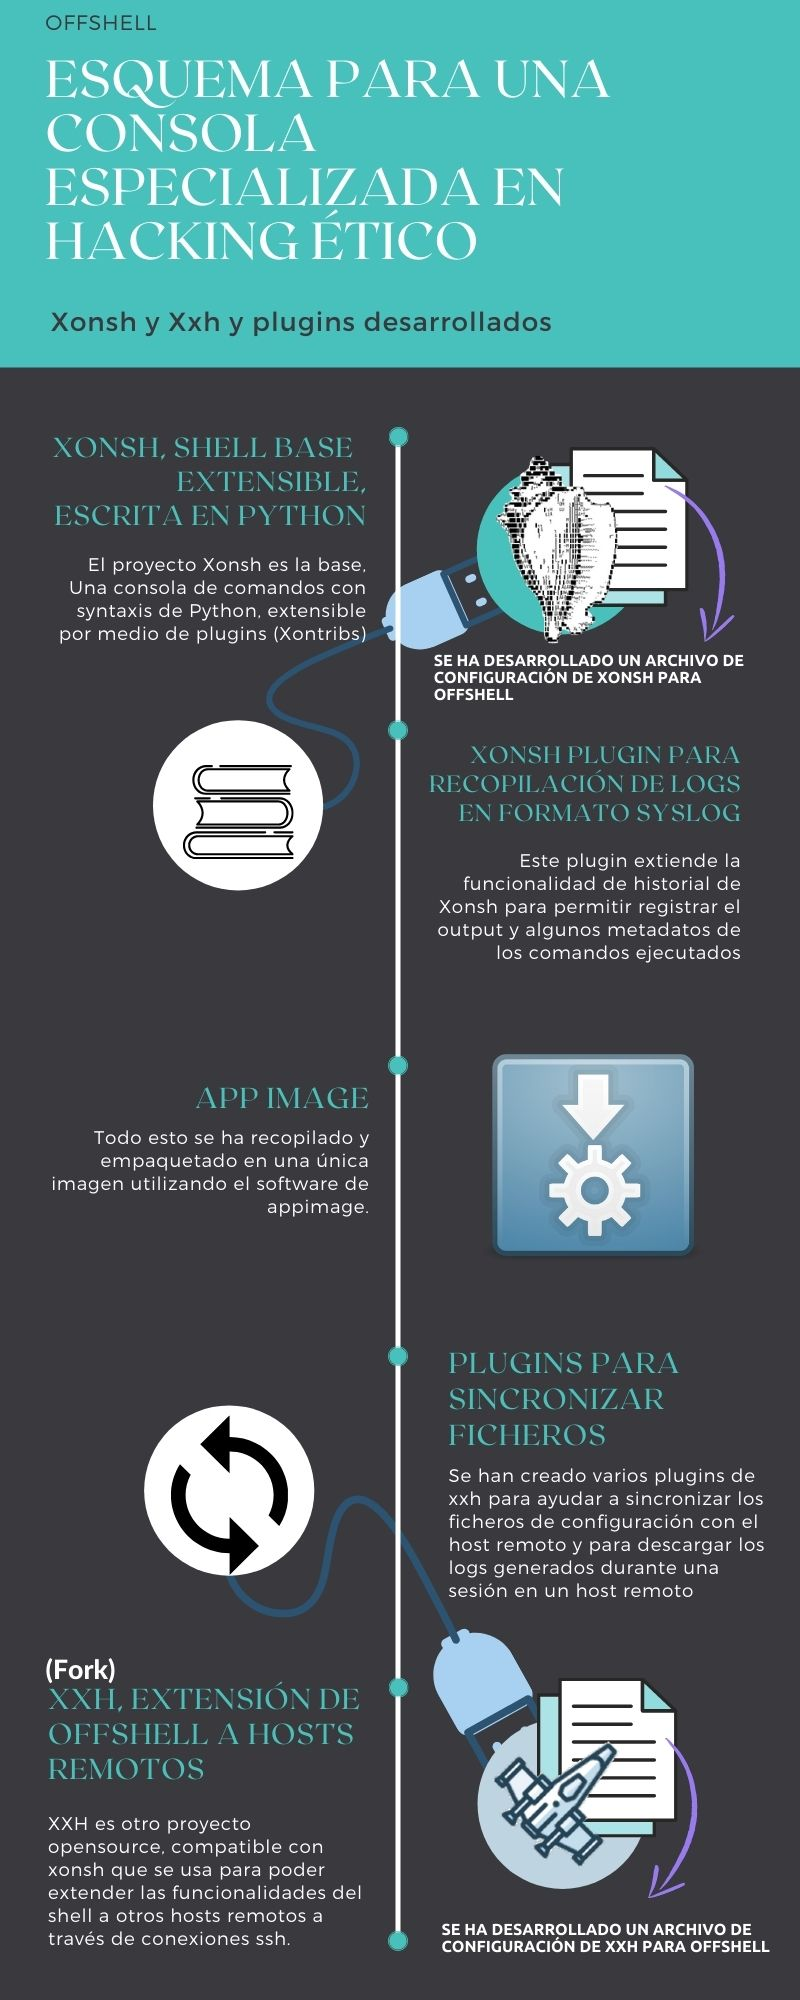
\includegraphics[width=0.5\textwidth]{imagenes/infografico.jpg}
  \caption{Gráfico con información de la estructura y extensiones del proyecto OffSh (Offensive Shell).}
  \label{infographic}
\end{figure}

Xonsh es una herramienta versátil, a la que se pueden añadir fácilmente plugins con nuevas funcionalidades. Es por ello que supone  \textbf{una buena oportunidad para la creación de una consola de comandos especializada en ciberseguridad}. 

Podemos, por tanto, definir una imagen de consola de comandos de offsh como un paquete instalable en cualquier sistrma operativo compatible con Python (que además, incluye una versión embebida de Python para evitar problemas con la versión del sistema operativo dónde se ejecuta), con soporte para usar XXH y archivos de configuración específicos (de Xonsh y XXH), plugins para ambos software y software adicional (por ejemplo, paquetes de python instalados en el python embebido, o binarios incluidos en el paquete con software específico para alguna tarea) que se encapsulan dentro de un paquete del tipo `appimage`.

Algunas de las ideas que se proponen para distinguir este de cualquier otro shell serían:

\begin{itemize}
    \item Un soporte específico para creación de \gls{reverse_shell} que permita crear fácilmente una conexión a través de xxh con un dispositivo en el que se consiga ejecutar código arbitrario, facilitando el acceso a determinadas herramientas dentro del mismo (como nmap u gobuster u otras herramientas útiles para analizar redes internas) y la experiencia de usuario (muy mala en muchas ocasiones por las condiciones visuales y de usabilidad de las shell inversas.
    \item Añadir utilidades de Python relacionadas con la ciberseguridad que se integren con la imagen de Xonsh específica para seguridad, de forma que sean accesibles sin necesidad de instalación. Programas típicos que no pesen mucho, alias, shortcuts, etc..
    \item Aprovechar que Xonsh tiene una base de \textbf{prompt\_toolkit} para añadir prompts dinámicos con información útil sobre los hosts analizados, colores para resaltar información importante, etc..
    \item Añadir scripts en pytest que realicen checks en el servidor en el que se ejecutan o en uno externo y generen alertas en Wazuh si se cumplen determinadas condiciones (automatización de la búsqueda de errores.
    \item Integraciones directas con softwares de ciberseguridad como Wazuh o Elastic SIEM.
\end{itemize}


\section{Simplificación de la instalación: appimage}

Para unificar todo el código desarrollado durante el trabajo tendríamos que conseguir algún tipo de`paquete' instalable que contuviera los siguientes elementos.

\begin{itemize}
    \item Una versión de Xonsh reciente
    \item El archivo de configuración diseñado.
    \item La versión de xxh desarrollada para el proyecto.
    \item El plugin de Xonsh para generar los registros.
    \item El plugin de xxh para descargar los registros externos.
    \item El plugin para analizar el output de determinados comandos.
    \item Otros plugins que puedan ser añadidos en un futuro.
\end{itemize}

Una solución a este problema sería introducir en el archivo de configuración de Xonsh el código necesario para instalar todas estas dependencias si no se encontraran instaladas. Sin embargo, esto tendría el inconveniente de hacer a Xonsh conectarse con hosts remotos para descargar código en la primera ejecución, y esto sería un aspecto negativo cuando se ejecuta Xonsh en una máquina a la que se ha accedido como parte de una auditoría (puesto que estas conexiones podrían ser detectadas).

Sin embargo, siguiendo la documentación de XXH se puede descubrir un elemento interesante: las \textbf{appimages}. Un tipo de empaquetación de software \textbf{portable y multiplataforma} que se puede utilizar sin necesidad de instalarlo ni de permisos de administrador en \textbf{cualquier sistema operativo}.

Xxh hace uso de estas \textit{appimages} para enviar un Xonsh portable y con un \textbf{Python embebido} que hace que podamos \textbf{ejecutar un shell Xonsh en cualquier dispositivo} sin necesidad de tener permisos de administrador o que Python esté instalado o actualizado en el host.

Del mismo modo, Xonsh ofrece un método de `instalación' basado en estas appimages y ofrece \textbf{medios para generar appimages personalizadas de Xonsh}-

Por tanto, la solución obvia parece ser \textbf{crear una appimage} de Xonsh con los elementos ya descritos, de forma que baste con descargarla y ejecutarla. Y que sea esta appimage la que se envía a los dispositivos remotos cuando se establece una conexión utilizando xxh.

Esto refuerza la idea mencionada en el punto anterior de \textbf{la oportunidad de crear un shell específico para penetración de sistemas} que sea portable y fácil de utilizar, y que además facilita la ejecución de código Python, que es un lenguaje muy utilizado en ciberseguridad y pentesting.

La imagen desarrollada, así como las instrucciones para utilizarlas se encuentran en el repositorio: \url{https://github.com/offsh/offsh}. 

\begin{figure}[!hbt]
  \centering
  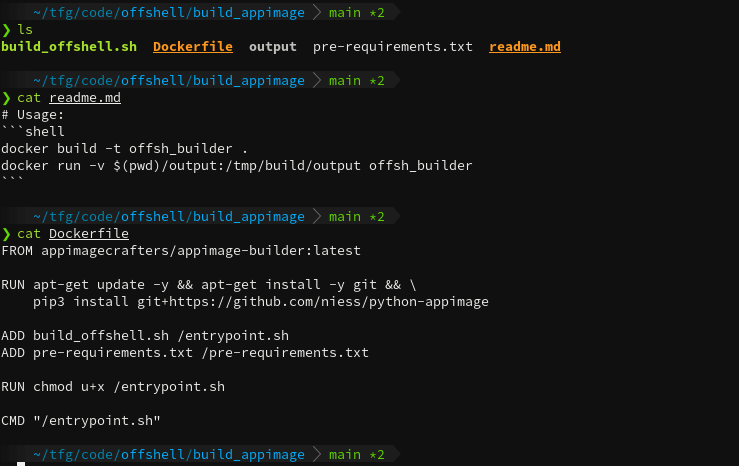
\includegraphics[width=\textwidth]{imagenes/build_appimage.png}
  \caption{Ejemplo de las herramientas y scripts disponibles en el repositorio para generar una nueva appimage de offsh usando Docker.}
  \label{appimage_build}
\end{figure}

La generación de nuevas versiones de la appimage se hace utilizando Docker (para simplificar la obtención de dependencias), tal y como se aprecia en la figura \ref{appimage_build}. Ver también figuras \ref{instructions} (instrucciones de instalación) y \ref{examplexonsh} (ejemplo de visualización de la consola de comandos).

\begin{figure}[!hbt]
  \centering
  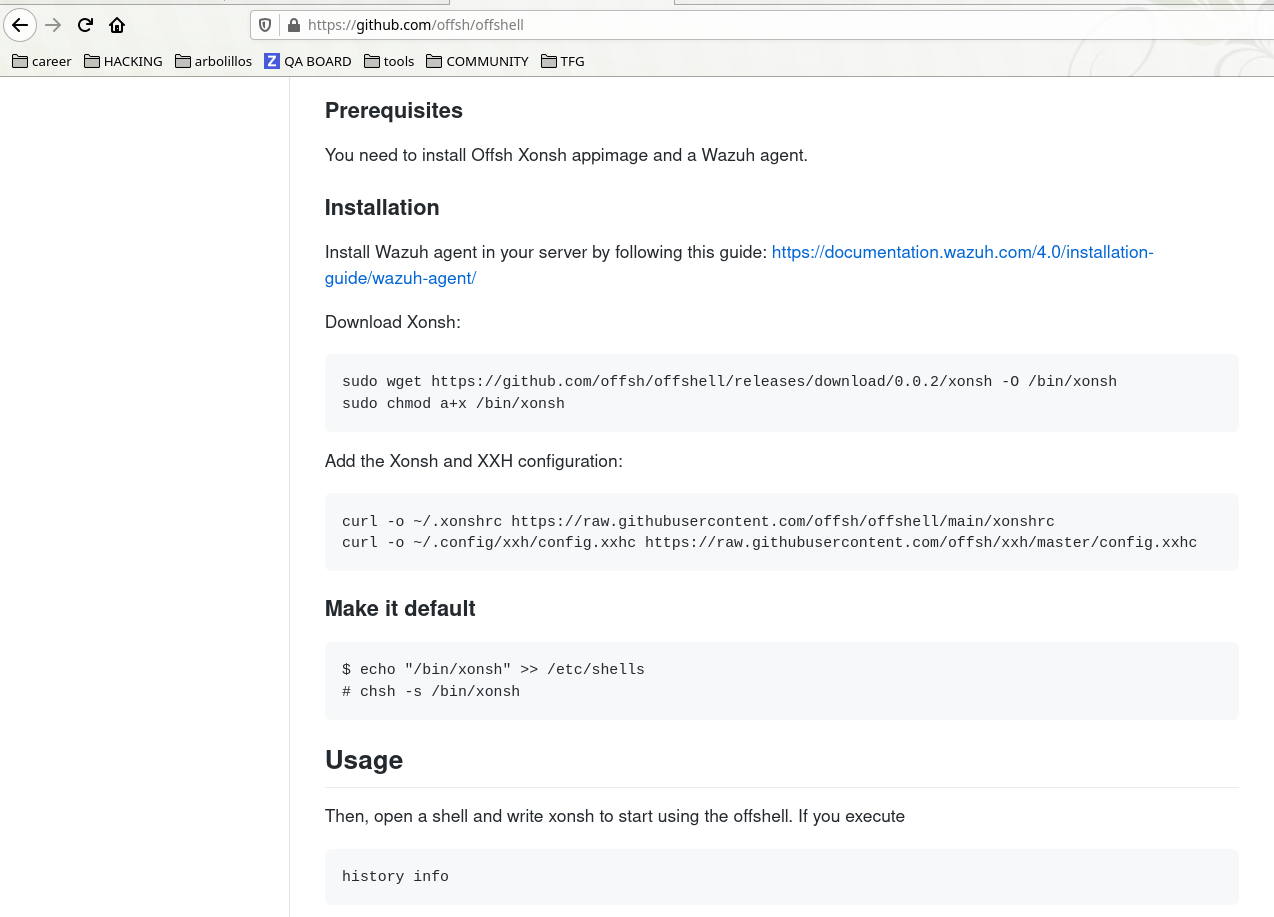
\includegraphics[width=\textwidth]{imagenes/offsh_instructions.png}
  \caption{Instrucciones de instalación y uso de la herramienta, disponibles en github}
  \label{instructions}
\end{figure}

\begin{figure}[!hbt]
  \centering
  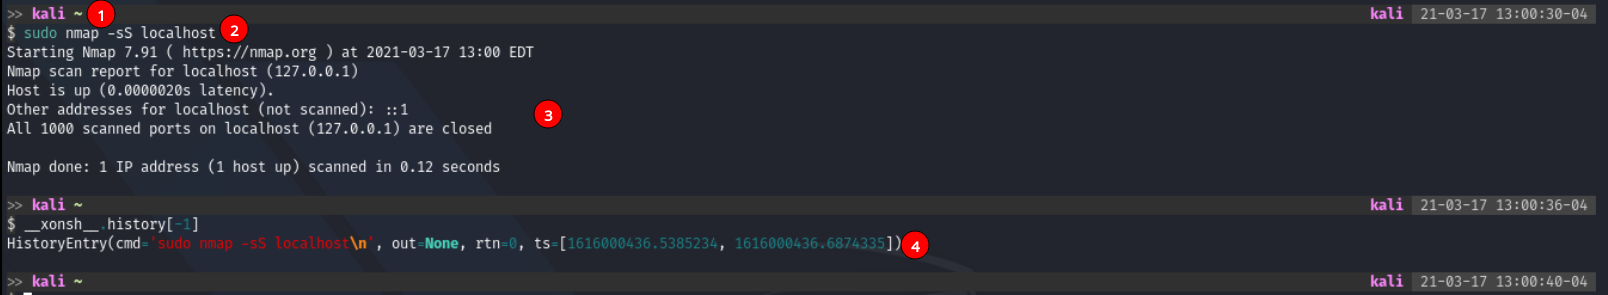
\includegraphics[width=\textwidth]{imagenes/offsh.png}
  \caption{Ejemplo del uso de offsh y la estructura de datos utilizada para almacenar la información de los comandos ejecutados. Se han introducido algunas mejoras visuales al promt de Xonsh por defecto (para diferenciarlo de otras sesiones normales de Xonsh y de otras consolas), como el prompt en barra y los colores según el usuario y el directorio (1). Se aprecia como el comando ejecutado (2) y su output (3) son almacenados en una base de datos que es accesible a través del propio shell (4)}
  \label{examplexonsh}
\end{figure}


\section{Propuesta de aplicación de Offsh para la docencia universitaria}

Para ahondar en la idea de que el proyecto desarrollado puede servir en distintos ámbitos además de en ciberseguridad (y que no se ha creado exclusivamente para ser usado como complemento de Wazuh), se ha decidido realizar una propuesta de aplicación real del mismo para docencia universitaria con ayuda del director de este trabajo, Alberto Guillén, profesor del Departamento de Arquitectura y Tecnología de Computadores que en el momento de la realización del trabajo es responsable de la asignatura de Ingeniería de Servidores.

Para ello, se han analizado los guiones de prácticas actuales de la asignatura y se ha valorado la posibilidad de añadirles el uso de una imagen de xonsh creada con el framework diseñado para el trabajo de forma que los alumnos puedan entender mejor algunos aspectos como:

\begin{itemize}
    \item Qué es un shell y qué diferencia a unos de otros
    \item Ideas básicas sobre archivos de configuración (de un shell, VIM, u otros softwares con archivos similares)
    \item Qué es una conexión ssh, qué implica y cómo puede llevarse a cabo por medio de programas más complejos como xxh
    \item Qué es una consola de comandos, TTY, 
\end{itemize}

\subsection{Propuesta de integración en las prácticas de la asignatura}

En la segunda práctica de la asignatura se trabaja el uso de SSH, la propuesta entonces es la siguiente: añadir una descripción básica de Xonsh y de offsh y xxh así como instrucciones para instalarlo y usarlo dentro de un sistema

\subsection{Desarrollo de competencias}

Con esta propuesta se pretende ayudar a que los alumnos adquieran las siguientes competencias:

\begin{itemize}
    \item Competencias específicas de la asignatura
    \begin{itemize}
        \item \textbf{R1. Capacidad para diseñar, desarrollar, seleccionar y evaluar aplicaciones y sistemas informáticos, asegurando su fiabilidad, seguridad y calidad, conforme a principios éticos y a la legislación y normativa vigente.}, ya que conocerán distintos tipos de shell y podrán elegirlos según sus necesidades y saber cómo configurarlos.
        \item \textbf{R5. Conocimiento, administración y mantenimiento de sistemas, servicios y aplicaciones informáticas.}, ya que los shell y las conexiones ssh son aspectos fundamentales dentro de la administración de sistemas.
    \item Competencias Transversales
    \begin{itemize}
        \item \textbf{ T2. Capacidad de organización y planificación así como capacidad de gestión de la
Información.}, ya que trabajan con mecanismos para registrar la información (Datos y metadatos) generada durante una sesión de ejecución de comandos en una shell.
    \end{itemize}
    \end{itemize}
\end{itemize}

Desde el punto de vista del profesorado, se podrían usar los logs generados por los alumnos para evaluar el cumplimiento de estas y otras competencias, por ejemplo, se podría pasar una batería de tests sobre el fichero de logs generado por cada alumnos para comprobar que, efectivamente, se han cumplido ciertos requisitos para superar las prácticas.

\input{capitulos/04_Test_Penetración}
\chapter{Conclusiones}

Para finalizar este trabajo se van a resumir, en este Capítulo, las conclusiones extraídas para los objetivos planteados al inicio del proyecto, así como aquellas ideas que se pueden extraer del uso de las herramientas desarrolladas durante el caso de uso práctico.

Se puede afirmar que se han cumplido los objetivos propuestos dentro del plan establecido: se ha recopilado y analizado la información necesaria para desarrollar las cuestiones a discutir y se han llevado a la práctica estas ideas por medio de un caso práctico de uso. Además, como trabajo extra, se ha diseñado un framework para generar imágenes portables de shells personalizadas y se ha hecho una propuesta de aplicación de estas imágenes para docencia universitaria.

En esencia, el objetivo que se planteó era discernir qué puede aportar Wazuh al hacking ético y viceversa. Además de analizar las posibles interacciones entre estos dos ámbitos y desarrollar software para favorecer dichas interacciones.

Por un lado, se ha analizado cómo Wazuh puede ser un complemento a la hora de recopilar información de interés para los hackers éticos. Se ha desarrollado un módulo que permite integrar la ejecución de comandos en la app de Wazuh, almacenando su salida y sus metadatos, de forma que podamos clasificar los comandos ejecutados según ciertos criterios en función de su nivel de importancia, el tipo de evento que generan (reconocimiento, escalado de privilegios, análisis de vulnerabilidades, etc...) u otros criterios.

Por otro lado, en el caso de uso practico ha quedado claro que \textbf{Wazuh no es capaz de detectar cualquier ataque posible con una configuración por defecto}, de hecho, hace falta pensar bien cómo se quiere tratar de detectar cada tipo de ataque. Es por ello, que hacer tests de penetración de sistemas sobre una máquina con Wazuh instalado \textbf{puede ser una muy buena forma de evaluar el rendimiento de Wazuh y encontrar formas de mejorar el software o su configuración específica en un sistema}.

Por tanto, podemos concluir que, efectivamente, Wazuh puede ser una buena herramienta para complementar las labores de hackers éticos y, del mismo modo, actividades como los tests de penetración o los Bug Bounties pueden servir para \textbf{evaluar el rendimiento de Wazuh en un entorno} (como se ha demostrado en el caso práctico), pudiendo un hacker ético \textbf{encontrar puntos sin analizar por Wazuh} que se pueden solucionar por medio de configuraciones extra, plugins, integraciones con otros softwares,... abriendo un camino con infinidad de posibilidades.

Como parte del trabajo se ha desarrollado un framework para generar imágenes portables de consolas de comandos basadas en Xonsh, a las que se puede añadir configuraciones específicas, herramientas y dependencias adicionales, además de plugins para extender la funcionalidad de Xonsh. Estas imágenes se pueden cargar en XXH de forma que sean utilizadas cuando se establezca una sesión SSH con un host remoto, permitiendo así integrar las herramientas y configuraciones que se pudieran necesitar (por ejemplo, como parte de una auditoría de ciberseguridad) también en los hosts remotos a los que se accede. Además, se ha demostrado que este framework puede ser utilizado en otros ámbitos además del de la ciberseguridad y se ha hecho una propuesta de aplicación del mismo en el ámbito docente en una asignatura del Grado de ingeniería informática de la Universidad de Granada.

Este es un \textbf{proyecto de código abierto} por lo que todo el trabajo está disponible y abierto para posibles futuros proyectos relacionados, para los cuales también se han hecho algunas propuestas de posibles trabajos futuros: plugins, configuraciones o recopilaciones de dependencias que podría ser interesante explorar. Este framework desarrollado no formaba parte de los objetivos iniciales pero se ha concluido que podía explotarse la idea y crear, junto con el resto del trabajo, una herramienta que pudiera ser utilizada con distintos fines (y no solo para la integración con Wazuh). 

Entre las ventajas de utilizar el framework desarrollado se destaca la posibilidad de homogeneizar el acceso a las máquinas, proporcionando una shell que se puede ejecutar en cualquier sistema operativo compatible con Python (incluso si no tiene Python instalado o tiene una versión muy vieja, puesto que la imagen generada incluye un Python embebido), incluyendo Windows, Solaris, HPUX, AIX, etc..., de forma que la experiencia de usuario sea \textbf{la misma independientemente del sistema operativo}.

En total, se han creado (o clonado y posteriormente modificado) \textbf{8 repositorios públicos} como parte de la organización creada para albergar todo el contenido desarrollado durante el proyecto. En total se han hecho cerca de 100 commits con más de \textbf{258435} líneas de código. 

Además, durante el desarrollo del trabajo \textbf{se ha colaborado activamente con dos proyectos open-source}, xonsh y xxh, se han abierto más de 15 issues varios pull request en estos y otros repositorios secundarios.

\begin{figure}[!hbt]
  \centering
  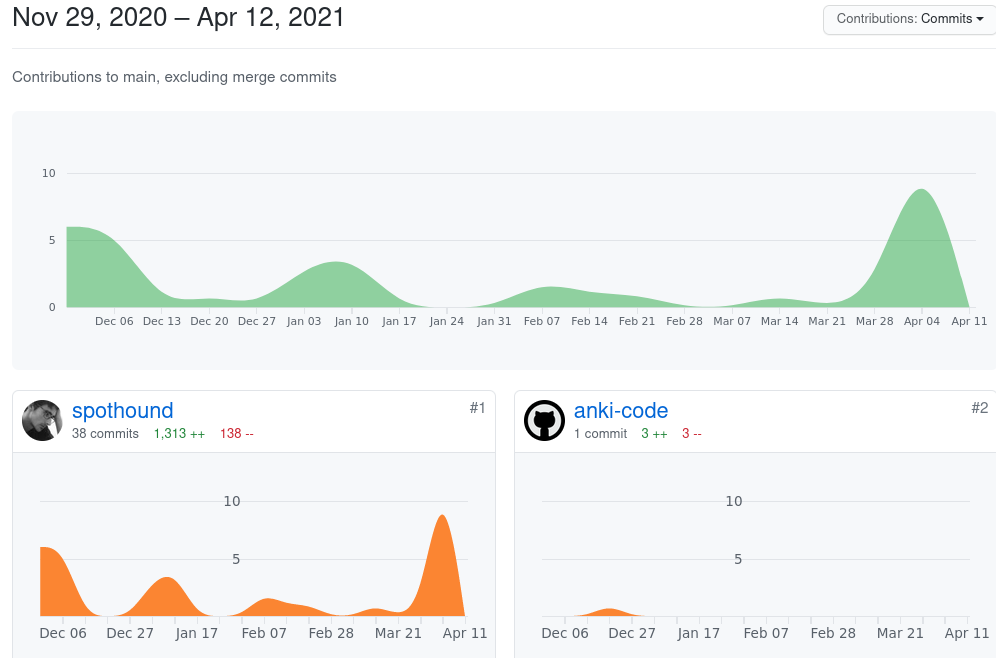
\includegraphics[width=\textwidth]{imagenes/github_activity.png}
  \caption{Visualización de la actividad del proyecto principal en github a lo largo del año en que se ha desarrollado el trabajo. Se puede apreciar que el proyecto incluso tiene una pequeña colaboración externa del \textbf{autor de xxh}. Aunque el número de commits o líneas de código no es muy elevado, se puede ver como el proyecto ha tenido actividad a lo largo de todo el año.}
  \label{githubactivity}
\end{figure}


Cabe destacar que \textbf{el autor de uno de estos proyectos se ha involucrado con el trabajo} creando algunas \textit{issues} con sugerencias para mejorar el proyecto e incluso abriendo un pull request (ver Figura \ref{githubactivity}).

En resumen, a lo largo del proyecto se han planteado una serie de hipótesis y experimentos para refutarlas que han sido llevados a cabo sin problema, se ha colaborado con proyectos open-source y se ha aportado a la comunidad creando una herramienta libre que además, se ha propuesto para ser utilizada en la docencia en la Universidad de Granada. 

Se ha cumplido el objetivo principal de analizar la relación entre Wazuh y el Hacking ético y se ha concluido que existen multitud de posibilidades para enlazar estos dos conceptos y sacar partido de su relación.


%
%%\chapter{Conclusiones y Trabajos Futuros}
%
%
%%\nocite{*}

\chapter{Apéndices}
\appendix
\input{capitulos/06_APÉNDICES}
\newglossaryentry{Malware}
{
    name=Malware,
    description={O software  `malicioso' es todo aquél programa o código que pretende (de forma intencionada) causar daños y/o sacar beneficios de un sistema}
}

\newglossaryentry{cloud}
{
    name=Cloud,
    description={La computación en la nube o \textit{cloud} (del inglés cloud computing), conocida también como servicios en la nube, informática en la nube, nube de cómputo o simplemente «la nube», es un paradigma que permite ofrecer servicios de computación a través de una red, que usualmente es internet}
}

\newglossaryentry{Ransomware}
{
    name=Ransomware,
    description={Es un tipo de \gls{Malware} que hace públicos o inaccesibles (por medio de encriptación, por ejemplo) los datos de la víctima con el objetivo de chantajearla para que pague un `rescate'}
}


\newglossaryentry{Reverse engineering}
{
    name={ingeniería inversa},
    description={Es una técnica que consiste en tratar de obtener por medios deductivos información sobre un producto o sistema haciendo uso del mismo y tratando de figurar como está diseñado}
}

\newglossaryentry{obfuscation}{
    name={obfuscation},
    description={Ofuscación, ocultación, anonimato. Es el acto de evitar ser descubierto mientras se realiza un ataque o una auditoría. Bien eliminando los rastros que se puedan dejar u ocultándolos por medio de falsos rastros que los escodan}
}

\newglossaryentry{network sniffing}
{
    name=network sniffing,
    description={Es la acción de atrapar y atender a todo el tráfico indiscriminado que circula por una red, sea cual sea su destinatario, con el objetivo de obtener algún tipo de información de interés}
}

\newglossaryentry{Rolling Release}
{
    name=Rolling Release,
    description={Es un tipo de distribución de Software en el que las actualizaciones son continuas en lugar de depender de un versionado discreto. Los cambios se van añadiendo de forma incremental conforme van siendo disponibles en lugar de ir emitiendo nuevas versiones con todos los cambios desde la anterior}
}

\newglossaryentry{compliance} 
{
    name=compliance,
    description={'el cumplimiento' de las normativas o leyes referentes a la seguridad de los datos que una empresa pueda almacenar o gestionar}
}

\newglossaryentry{vagrant}
{
    name=Vagrant,
    description={'una herramienta diseñada para el despliegue y configuración de entornos de máquinas virtuales (utilizando diversos proveedores como virtualbox, qemu, aws, etc}
}

\newacronym{ddos}{DDOS}{Distributed Denial Of Service}

\newacronym{aws}{AWS}{Amazon Web Service}


\newacronym{iot}{IOT}{The Internet of Things}

\newglossaryentry{OpenSource}
{
    name=OpenSource,
    description={OpenSource o código abierto es un tipo de software liberado con una licencia que asegura el derecho de los usuarios a usar, estudiar, cambiar y distribuir el mismo con cualquier propósito}
}

\newglossaryentry{Pull Request}
{
    name=Pull Request,
    description={Una Pull Request es la acción de validar un código que se va a mergear de una rama a otra. Por ejemplo, de una rama de desarrollo en un Fork de un proyecto a una rama oficial}
}

\newglossaryentry{Fuzzing}
{
    name=Fuzzing,
    description={Según la OWASP, fuzzing es el acto de introducir datos mal formados en un programa con el objetivo de conseguir un comportamiento en este inesperado. Aplicado, por ejemplo, al ámbito de web, podríamos considerar fuzzing las técnicas de SQL injection y similares, dónde se introduce código SQL en lugares como los credenciales de acceso para conseguir logearse con un usuario distinto al que poseemos}
}

\newglossaryentry{syslog}
{
    name=Syslog,
    description={syslog es un estándar para el envío de mensajes de registro (logs) en una red informática IP. Por syslog se conoce tanto al protocolo de red como a la aplicación o biblioteca que envía los mensajes de registro. Un mensaje de registro suele tener información sobre la seguridad del sistema, aunque puede contener cualquier información. Junto con cada mensaje se incluye la fecha y hora del envío}
}

\newglossaryentry{phishing}
{
    name=Phishing,
    description={Técnica empleada por delincuente cibernéticos para estafar y obtener información de sus víctimas haciéndose pasar por otra persona o entidad (a través de correo electrónico, redes sociales, etc}
}


\newacronym{IaC}{IAC}{Infrastructure as Code}
\newacronym{CPA}{CPA}{Certified Public Accountant}
\newacronym{FOSS}{FOSS}{Free & Open-Source Software}

\newglossaryentry{forensics}
{
    name=forensics,
    description={Es el término que describe a las acciones llevadas a cabo para recopilar información de los sistemas informáticos que pueda ser utilizada para demostrar hechos por ejemplo durante una investigación relacionada con un crimen cibernético}
}

\newglossaryentry{antiforensics}
{
    name=anti-forensics,
    description={Técnicismo que se emplea para referise a aquellas acciones llevadas a cabo para dificultar las labores de investigación forense (forensics \gls{forensics}) de los equipos de seguridad de una empresa. Borrar u ocultar los rastros que se pueda haber dejado durante la explotación de vulnerabilidades de un sistema con el objetivo de imposibilitar el descubrimiento del mismo por parte de los administradores del sistema}
}

\newglossaryentry{siem}
{
    name=SIEM,
    description={`Security Information and Event Management', es un tipo de software que permite recopilar y analizar información de seguridad de distintos dispositivos, alertando al usuario de aquellos eventos importantes que tengan lugar}
}


\newglossaryentry{HIDS}
{
    name=HIDS,
    description={`Host Based Intrussion Detection System', es un tipo de software que permite detertar intentos de intrusiones en un sistema y reportarlas}
}

\newglossaryentry{mitre}
{
    name=MITRE ATT\&ACK,
    description={Una base de datos pública de conocimiento de tácticas de `ataques adversarios' que trata de modelar y agrupar las distintas acciones que puede llevar a cabo un criminar para dañar a una entidad}
}

\newglossaryentry{fork}
{
    name=fork,
    description={También llamado `bifurcación' en español. Es el desarrollo de un proyecto informático tomando como base el código fuente de uno ya existente o de alguna ramificación de este. Un ejemplo claro de esto son las distintas diburcaciones de desarrollo de las distribuciones de Linux, dónde Ubuntu, por ejemplo, es una bifurcación o un fork de Debian}
}

\newglossaryentry{reverse_shell}
{
    name=Consola inversa,
    description={O en inglés `reverse shell'. Es un tipo de conexión entre dos hosts que ocurre de forma opuesta a la habitual: desde el dispositivo que se va a conectar se abre una aplicación que `espera' una conexión y desde el dispositivo que va a ser accedido se abre una consola de comandos que se conecta a dicha aplicación. Es una técnica que se utiliza en el ámbito de la ciberseguridad para conseguir acceso remoto a dispositivos dónde podemos ejecutar código arbitrario de algún modo}
}

\newglossaryentry{bugb}
{
    name=Bug Bounty,
    description={Son programas en los que empresas u organizaciones ofrecen importantes recompensas económicas a aquellas personas (ajenas a la organización) capaces de encontrar vulnerabilidades o errores de seguridad en alguno de sus sistemas.}
}
\addcontentsline{toc}{chapter}{Glosario}
\printglossary

\medskip

\printbibliography


\end{document}
